% !TEX encoding = UTF-8 Unicode 
%
% Use:
% magister / inzynier - for master thesis or engineering thesis
% druk / archiwum - for print version or archive version
% en - to translate template into english
% examples:
%\documentclass[inzynier,druk,en] - master thesis, print version, english
%\documentclass[magister,druk,en]{dyplom}
%\documentclass[magister,druk]{dyplom}

\documentclass[magister,druk]{dyplom}

\usepackage[utf8]{inputenc}
\usepackage{hyperref}
\usepackage{tocvsec2}
\usepackage{subcaption}
\usepackage{url}
\usepackage[acronym]{glossaries}

% Define URL text wrap points
\def\UrlBreaks{\do\/\do-}

% Maximum section's depth.
\setcounter{secnumdepth}{4}

% Listings settings
\setminted{breaklines, 
frame=lines,           
framesep=3mm,          
baselinestretch=1.1,   
fontsize=\small,       
% linenos              % line numbering
}

\usepackage{lipsum}
\usepackage{pgfplots}
\pgfplotsset{compat=newest}

% \faculty{Faculty of \dots}                   % Uncomment if applicable
\fieldofstudy{Informatyka Stosowana}                          
\author{Kajetan Pynka}
\title{Badanie wykorzystania sztucznej inteligencji w procesie tworzenia dostosowującej się do użytkownika narracji w grach komputerowych}
\supervisor{Dr Maciej Walczyński}
% \consultant{Consultant's name}               % Uncomment if applicable
\specialisation{Projektowanie Systemów Informatycznych}                         % Uncomment if applicable
\keywords{słowo1, słowo2, słowo3}   % 3-5 keywords  

\makenoidxglossaries
\loadglsentries{glossary/glossary}

\begin{document}

\maketitle

\abstract{
    % Polskie streszczenie
    W niniejszej pracy zbadano potencjał wykorzystania dużych modeli językowych (\gls{llm}) do poprawy jakości narracji
    i zaangażowania graczy w grach typu "visual novel". Wykorzystano system generujący dialogi na podstawie \gls{llm}, który
    następnie zaimplementowano w prototypowej grze. Przeprowadzono badania z udziałem graczy, w których oceniano
    imersję narracyjną, zaangażowanie oraz ogólną satysfakcję z gry w wersji z dialogami generowanymi przez \gls{llm} oraz
    wersji z wcześniej zdefiniowanymi dialogami. Wyniki badań wykazały, że uczestnicy odczuwali większą satysfakcję
    oraz zainteresowanie podczas interakcji z \gls{npc} zarządzanymi przez \gls{llm}. Potwierdziło to tezę, że wykorzystanie
    dużych modeli językowych może skutecznie podnieść jakość narracji w grach
    poprzez dostarczanie bardziej zindywidualizowanych i responsywnych doświadczeń dla graczy. Praca omawia również
    potencjalne dalsze kierunki badań i rozwoju systemów opartych na \gls{llm} w kontekście gier wideo.
}{
    % English abstract
    This work investigated the potential of utilizing large language models (\gls{llm}s) to enhance narrative quality
    and player engagement in visual novel-style games. A system for generating dialogues based on \gls{llm}s was used
    in a prototype game. Player studies were conducted to evaluate narrative immersion, engagement,
    and overall game satisfaction in both the \gls{llm}-generated dialogue version and a version with predefined dialogues.
    The results showed that participants experienced greater satisfaction and interest in interacting with the
    \gls{llm}-operated \gls{npc}s. This confirmed the
    hypothesis that leveraging \gls{llm}s can effectively improve narrative quality in games by providing more
    individualized and responsive experiences for players. The work also discusses potential further research
    directions and the development of \gls{llm}-based systems in the context of video games.
}

\tableofcontents

\settocdepth{chapter}

% !TEX encoding = UTF-8 Unicode 
% !TEX root = praca.tex

\chapter*{Wstęp}\label{chapter:introduction}

Narracja i immersyjne doświadczenia w grach wideo stają się coraz ważniejsze dla graczy. Tworzenie angażujących
i spójnych historii pozostaje jednak wyzwaniem dla deweloperów gier. Wykorzystanie zaawansowanych technologii,
takich jak duże modele językowe (LLM), może potencjalnie rozwiązać te problemy i podnieść jakość narracji w grach.

\section*{Zakres pracy}

Niniejsza praca koncentruje się na zbadaniu, w jaki sposób włączenie dużych modeli językowych (LLM) do gry
typu „visual novel" może zwiększyć imersję narracyjną i zaangażowanie gracza. Praca obejmuje implementację systemu
generującego dialogi na podstawie LLM oraz przeprowadzenie badań z udziałem graczy w celu oceny skuteczności
proponowanego rozwiązania.

\section*{Cel pracy}

Celem tej pracy jest zbadanie, w jaki sposób włączenie dużych modeli językowych (LLM) do gry typu „visual novel"
może zwiększyć imersję narracyjną i zaangażowanie gracza. Główną tezą jest to, że interaktywne dialogi generowane
przez LLM zapewnią bardziej spójną i dostosowaną do gracza narrację w porównaniu z wcześniej zdefiniowanymi
dialogami, co przełoży się na większe zaangażowanie i satysfakcję z gry.

\section*{Struktura pracy}

Praca podzielona jest na cztery rozdziały, podsumowanie oraz wnioski. Pierwszy rozdział przedstawia kontekst i
znaczenie narracji w grach wideo oraz omawia potencjalne korzyści wynikające z wykorzystania LLM. Drugi rozdział
przegląda istniejące prace związane z generowaniem narracji i dialogów w grach. Trzeci rozdział opisuje szczegóły
implementacji zaproponowanego systemu. W czwartym rozdziale przedstawione są wyniki badań z udziałem graczy oraz
analiza skuteczności rozwiązania. Praca kończy się podsumowaniem, wnioskami oraz wskazaniem możliwych kierunków
dalszych badań.

\settocdepth{subsection}

% !TEX encoding = UTF-8 Unicode 
% !TEX root = praca.tex
\graphicspath{{chapters/chapter1/imgs/}}

\chapter{Narracja w grach}\label{chapter:ch1}

Niniejszy rozdział ma na celu dokonanie przeglądu gier komputerowych na przestrzeni lat, ze
szczególnym naciskiem na ewolucję sposobów oraz form narracji przedstawianych w tych grach.
Wyszczególnione zostaną również naistotniejsze struktury i rodzaje narracji, które są współcześnie
wykorzystywane. Dodatkowo, nastąpi krótki przegląd najpopularniejszych technik prezentacji narracji.
Na koniec nakreślone zostaną systemy dialogowe wykorzystywane przez gry komputerowe.

\section{Historia narracji w grach komputerowych}\label{section:ch1_1}

Aby zrozumieć istotę narracji w grach komputerowych, należy przede wszystkim określić
co może kryć się pod tym pojęciem. Pozwoli to dokonać przeglądu wybranych tytułów
i wyciągnąć z tego przeglądu wnioski. Żeby udowodnić rozwój w sposobie prezentowania narracji
na przestrzeni lat, prześledzone zostały części jednej z serii gier --- \textit{"Final Fantasy"} ---
wydawanej od roku 1987.

\subsection{Definicja narracji}\label{subsection:ch1_1_1}

Pojęcie narracji i samo jej występowanie w grach komputerowych jest kwestią sporną
w literaturze od lat. Barry Ip, w swojej pracy \cite{narrative_structures}, dokonuje wyróżnienia trzech słów ściśle
powiązanych ze sobą: \textit{historia}, \textit{fabuła} oraz \textit{narracja}. Na potrzeby jego
badań historia zdefiniowana została następująco:

\begin{quotation}
	\ldots \textit{sekwencja zdarzeń obejmujących byty.} \cite{narrative_structures}
\end{quotation}

Związana z historią jest również fabuła, która została określona przez Arystotelesa jako:

\begin{quotation}
	\ldots \textit{organizacja zdarzeń.} \cite{narrative_structures}
\end{quotation}

Sama narracja, ściśle powiązana z dwoma poprzednimi terminami, wyrażona została w sposób
następujący:

\begin{quotation}
	\ldots \textit{reprezentacja zdarzenia lub serii zdarzeń.} \cite{narrative_structures}
\end{quotation}

W ramach tej pracy, można przyjąć wszystkie te pojęcia jako istotne i na tyle bliskie
siebie, że mogą być wykorzystywane zamiennie.

Jakub Majewski sugeruje, że debatowanie nad istnieniem narracji jest odpowiednie dla niektórych
gier, a dla niektórych nie \cite{theorising_narrative}. Rozdzielenie bowiem tych form
przekazu, które można zaliczyć do treści fabularnej, nie jest takie oczywiste. Przytoczyć można
przykład \textit{Space Invaders} (1977) --- gra nie przytacza żadnego opisu w formie tekstowej,
skupiając się wyłącznie na rozgrywce. Na podstawie samego tytułu można jednak
przypuścić, że dokonuje się pewnego rodzaju inwazja, a stoją za nią przybysze z kosmosu \cite{theorising_narrative}.

Ten przykład pokazuje, że granica między grami posiadającymi narrację a tymi, w których jest ona nieobecna,
może być płynna. Nawet gry pozbawione bezpośrednich opisów fabularnych mogą zawierać pewne nawiązania narracyjne,
które wynikają z innych elementów, takich jak tytuł czy grafika. W związku z tym, podział na gry z narracją i bez
narracji może być problematyczny, ponieważ elementy narracyjne mogą przejawiać się w różnych formach i stopniach
w różnych grach. Jako że nie jest to główny problem poruszany w niniejszej pracy to wszystko co może być elementem
narracyjnym, jest za taki uznawany.

Do budowania narracji w grach wykorzystane mogą być wzorce znane z literatury. Przykładem takiego wzorca jest
\textit{"Podróż bohatera"}\cite{narrative_structures}, który opisuje 12 kluczowych etapów, odgrywających
istotną rolę w budowie angażujących historii (Tabela \ref{tab1:ch1_1_1}). Blisko powiązana z \textit{"Podróżą bohatera"}
jest znana struktura trzech aktów opisana przez Arystotelesa, która zakłada podział utworu na
początek, środek i koniec\cite{narrative_structures}. Jest to bardzo elastyczna a zarazem bardzo ogólna metoda
podziału. Zasadniczo w każdym utworze dałoby się bowiem w pewien sposób wyodrębnić te akty.

Struktury te pozwalają projektantom fabuły konstruować spójny świat fikcji --- niezależnie od formy w
jakiej zostanie zaprezentowana odbiorcom. Takowa może być adaptowana zarówno do powieści, jak i do materiału
filmowego czy też gier komputerowych.

\begin{table}[h!]
	\caption{Dwanaście etapów wzorca narracyjnego "Podróży bohatera" \cite{narrative_structures}}
	\label{tab1:ch1_1_1}
	\begin{center}
		\begin{tabular}{p{1.5in} p{4in}}
			\hline
			Etap                                & Opis                                                                                                                                                                                                                                                                                                                            \\
			\hline
			1. Zwyczajny świat                  & Gracz po raz pierwszy spotyka bohatera i zapoznaje się z jego pochodzeniem, zazwyczaj za pośrednictwem historii drugoplanowej                                                                                                                                                                                                   \\
			2. Wezwanie do przygody             & Wskazówka, że bohater opuści zwykły świat, by rozpocząć nową przygodę. Ten etap działa jak katalizator, który uruchamia główny wątek fabularny                                                                                                                                                                                  \\
			3. Odrzucenie wezwania              & W tradycyjnej strukturze monomitu bohater odrzuca początkową propozycję opuszczenia zwykłego świata i rozpoczęcia misji, zwykle w chwili wątpliwości lub niepewności                                                                                                                                                            \\
			4. Spotkanie z mentorem             & Gdy bohater decyduje się na podjęcie zadania, mentor dostarcza mu informacji potrzebnych do podjęcia decyzji. Mentorem może być wszystko, co dostarcza informacji - brodaty starzec, robot, biblioteka, doświadczenia z przeszłości i tak dalej                                                                                 \\
			5. Przekroczenie pierwszego progu   & Bohater przechodzi z bezpiecznego zwykłego świata do nowego, niebezpiecznego i nieznanego świata poszukiwań                                                                                                                                                                                                                     \\
			6. Testy, sprzymierzeńcy i wrogowie & Faza ta jest zwykle największą częścią fabuły gry, ponieważ gracz poznaje wszystkie główne postacie                                                                                                                                                                                                                             \\
			7. Podejście do najgłębszej jaskini & Jest to miejsce, w którym bohater znajduje nagrodę, której szuka - taką jak zdobycie niezbędnej umiejętności, broni lub opanowanie wszystkiego, co napotkał do tej pory. Zazwyczaj ma to miejsce pod koniec gry. Głównym celem tej części historii jest przygotowanie bohatera do ostatecznej bitwy                             \\
			8. Próba                            & To tutaj bohater staje do ostatecznej walki ze swoim nemezis lub "ostatecznym bossem". Nemezis może pojawić się jako byt fizyczny (osoba lub przedmiot) lub niefizyczny (czas, intensywność lub trudność)                                                                                                                       \\
			9. Nagroda                          & Wiele gier kończy się w tym momencie, gdy wróg zostaje pokonany, a nagrodą jest zazwyczaj końcowa cut-scenka opisująca, co dzieje się z bohaterem po jego triumfie                                                                                                                                                              \\
			10. Droga powrotna                  & Niektóre gry pozwolą graczowi powrócić do zwykłego świata po otrzymaniu nagrody, ale może nie być możliwe, aby bohater z powodzeniem zintegrował się ze starym światem                                                                                                                                                          \\
			11. Wksrzeszenie                    & Ta część historii odpowiada na wszelkie pytania bez odpowiedzi, takie jak konsekwencje misji, potencjalne konflikty, które mogą pojawić się w przyszłych sequelach, lub wszelkie testy, którym bohater musi stawić czoła przed końcem. Może mieć również formę ostatecznego zwrotu akcji, jako coś nieoczekiwanego przez widzów \\
			12. Powrót z nagrodą                & Jest to ostatni etap historii, w którym bohater w końcu powraca do zwykłego świata i widzi korzyści płynące z jej nagrody. Bohater może porównać swoje życie przed i po wyprawie, aby zobaczyć, jak wszystko się zmieniło                                                                                                       \\
			\hline
		\end{tabular}
	\end{center}
\end{table}

\newpage

\subsection{Przedstawienie narracji w grach na przestrzeni lat}\label{subsection:ch1_1_2}

Kamienie milowe w początkach branży gier wideo to: Spacewar (Rys \ref{fig:ch1_1_2_spacewar}) - pierwsza interaktywna gra z
1962 roku, Magnavox Odyssey (1972) - pierwszy domowy system gier podłączany do telewizora, a
także Pong (Rys \ref{fig:ch1_1_2_pong}) od Atari (1972) i przenośne gry LED Mattela (1977)\cite{the_evolution_of_video_games}.

Gra "Spacewar" (Rys \ref{fig:ch1_1_2_spacewar}) przedstawia dwa statki kosmiczne, które w obrębie studni potencjału grawitacyjnego ("gravity well")
prowadzą ze sobą starcie. Jeden ze statków nazywany jest "igłą" a drugi "klinem". Oba są sterowane przez
graczy, którzy mają do dostępu ograniczoną amunicję i paliwo do nawigowania. Cała rozgrywka prowadzona jest
na planszy 2-wymiarowej, gdzie tło stanowią gwiazdy. Gra nie posiada żadnej formy narracji, natomiast była
istotnym elementem dalszego rozwoju branży.

\begin{figure}[h]
	\caption{Spacewar (1962)}
	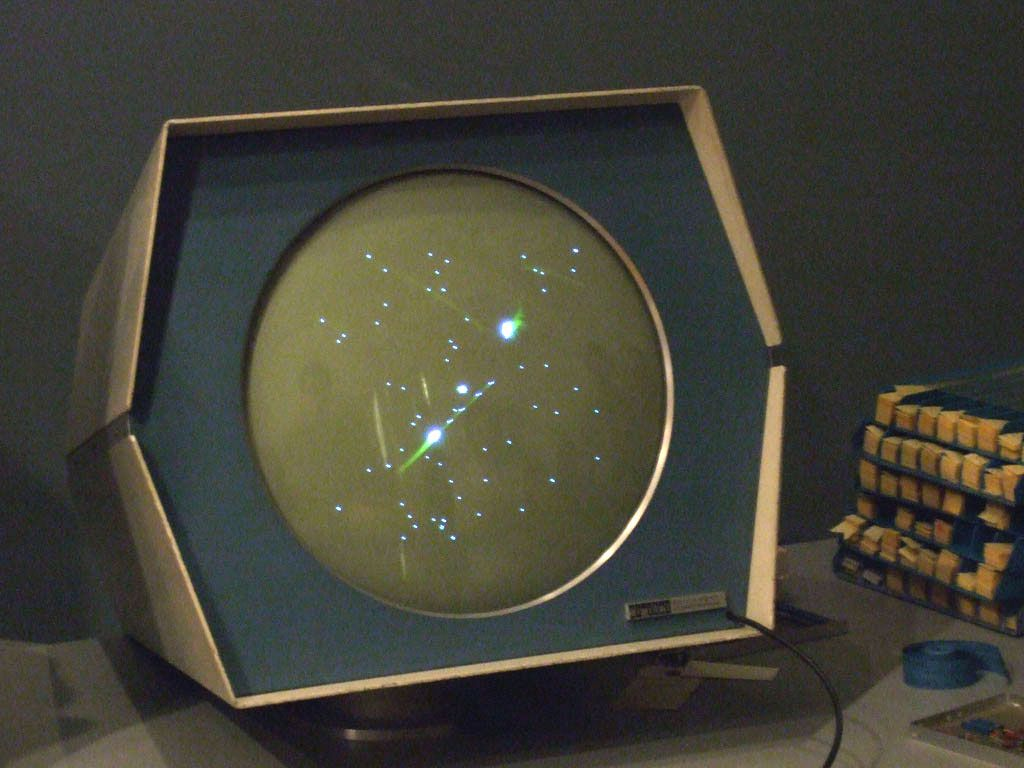
\includegraphics[width=0.5\textwidth]{ch1_1_2_spacewar.jpg}
	\centering
	\label{fig:ch1_1_2_spacewar}
\end{figure}

W ramach rozgrywki w "Pong" (Rys \ref{fig:ch1_1_2_pong}) mamy do czynienia z symulatorem tenisa stołowego. Dwójka graczy steruje paletkami
poruszającymi się pionowo. Za pomocą tych paletek odbijają piłkę na stronę przeciwnika. Jeśli ten nie odbije
jej z powrotem, to uderzający zdobywa punkt. Wygrywa pierwszy gracz, który uzyska 11 punktów. Podobnie jak
w przypadku "Spacewar", "Pong" nastawiony jest na rozgrywkę dwuosobową i nie posiada żadnej formy narracji.

\begin{figure}[h]
	\caption{Pong (1972)}
	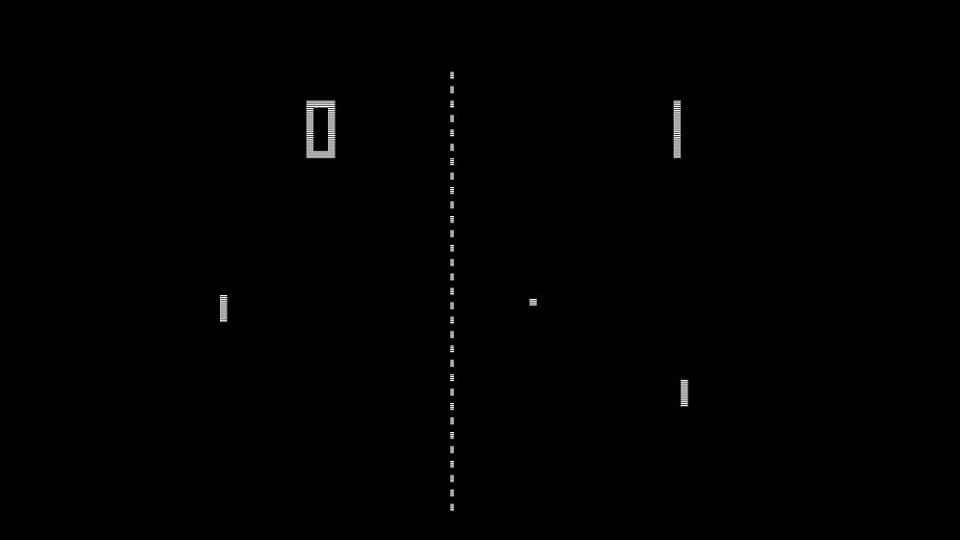
\includegraphics[width=0.5\textwidth]{ch_1_1_2_pong.jpg}
	\centering
	\label{fig:ch1_1_2_pong}
\end{figure}

Lata 70. przyniosły rozwój firm jak Atari, Nintendo i Sega oraz pierwsze hity salonów
gier np. Pacman (1980), który sprzedał 300 000 sztuk na całym świecie\cite{the_evolution_of_video_games}.

W "Breakout" (Rys \ref{fig:ch1_1_2_breakout}) gracz steruje paletką poruszającą się poziomo i stara się zniszczyć położoną wyżej ścianę
z cegiełek. Ściana składa się z ośmiu rzędów kolorowych bloczków. Używając pojedynczej piłki należy
zbić jak najwięcej cegiełek (przy kontakcie piłki z cegiełką zostaje ona zniszczona). Grający posiada
trzy życia i w ramach nich musi wyczyścić dwie ściany. Gracz traci życie jeśli nie odbije piłki wracającej
do niego. Rozgrywka ta została zaplanowana na maszyny \textit{arcade} z myślą o zdobywaniu jak najwięcej
punktów. Nie da się dostrzec w jej przypadku żadnej formy fabuły.

\begin{figure}[h]
	\caption{Breakout (1976)}
	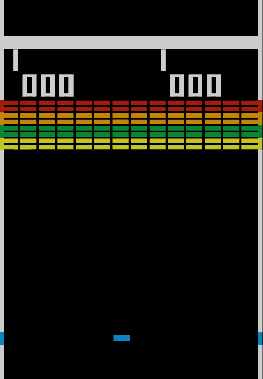
\includegraphics[width=0.5\textwidth]{ch1_1_2_breakout.jpg}
	\centering
	\label{fig:ch1_1_2_breakout}
\end{figure}

"Space Invaders" (Rys \ref{fig:ch1_1_2_space_invaders}) to gra akcji opracowana i wydana w Japonii przez Taito. Gracz steruje działem laserowym
umieszczonym na dole ekranu, które porusza się poziomo. Kosmici ułożeni w 5 rzędów po 11 obiektów
przemieszczają się grupowo w lewo i prawo, schodząc niżej gdy dotkną krawędzi ekranu. Celem gry jest
zestrzelenie wszystkich kosmitów przez gracza, posiadającego trzy życia. Obcy wystrzeliwują swoje pociski,
które przy trafieniu w gracza zabierają mu jedno życie. Gra kończy się natychmiastowo w momencie gdy
najeźdźcy dotrą do dołu ekranu. Tak jak w przypadku "Breakout" mamy do czynienia z rozgrywką nastawioną na
maszyny \textit{arcade}, a co za tym idzie na zdobywanie punktów. Oprócz kwestii poruszanych w
podsekcji \ref{subsection:ch1_1_1}, nie występują inne przesłanki fabularne.

\begin{figure}[h]
	\caption{Space Invaders (1978)}
	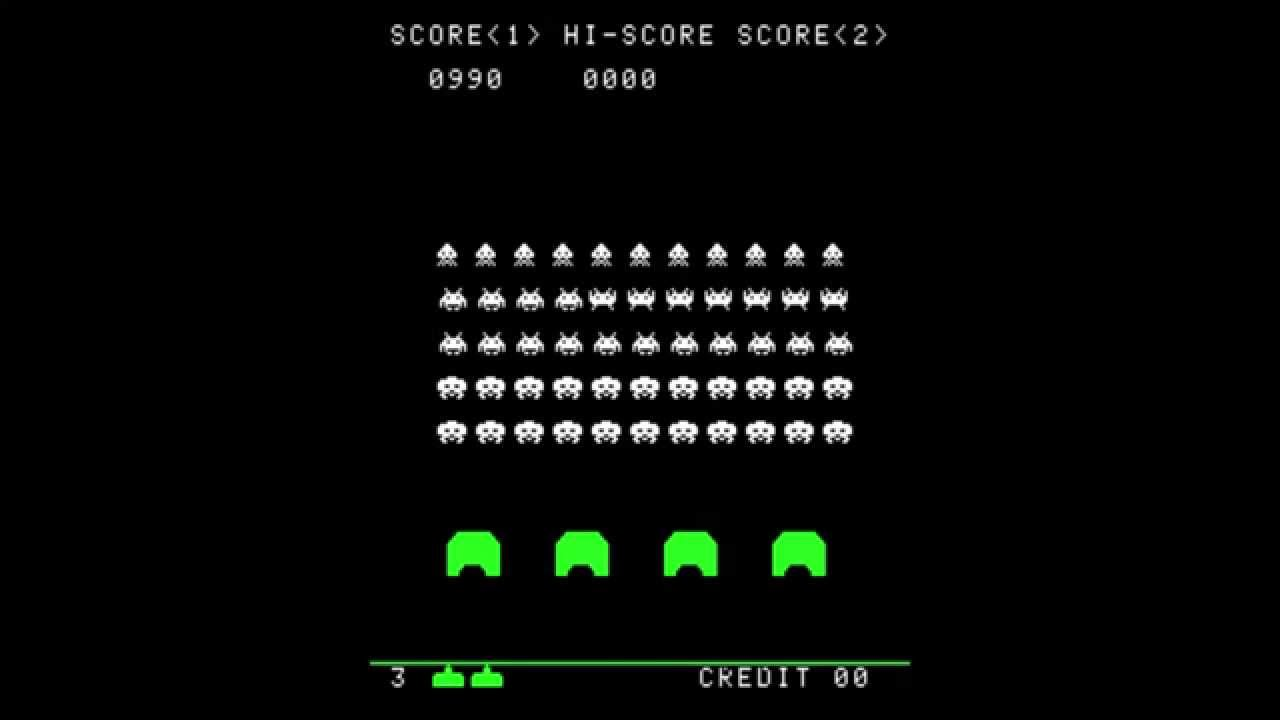
\includegraphics[width=0.5\textwidth]{ch_1_1_2_space_invaders.jpg}
	\centering
	\label{fig:ch1_1_2_space_invaders}
\end{figure}

\newpage

W latach 80. nastąpił boom konsol domowych - Nintendo NES, Sega Master System, Atari 7800\cite{the_evolution_of_video_games}.
Obecnie kiedy większość graczy myśli o grach \textit{retro} to ma na myśli między innymi właśnie tytuły
wyprodukwane na te serie konsol.

Jedną z najbardziej znanych w popkulturze gier jest "Super Mario Bros." (Rys \ref{fig:ch1_1_2_super_mario_bros}).
Gracz wciela się w rolę tytułowego Mario (w wersji jednoosobowej), który ma jako główne zadanie obrane
ocalenie księżniczki. W tym celu pokonuje kolejne krainy (poziomy) oraz przeciwników. Gra składa się z ośmiu
światów, gdzie każdy z nich jest dodatkowo podzielony na cztery poziomy. Mamy więc do czynienia z
wielopoziomową formą rozrywki, gdzie światy różnią się między sobą ze względu na warstwę wizualną, dźwiękową
jak i ze względu na występujących przeciwników czy przeszkody. Są to pewnego rodzaju zalążki narracji
(która została wykreowana przez świat). Jedyną formą pisemnej fabuły jest tekst występujący po ukończeniu
poziomu (Rys \ref{subfig:ch_1_1_2_mario_2}).

\begin{figure}[h]
	\begin{subfigure}{0.49\textwidth}
		\caption{Ekran tytułowy}
		
\includegraphics[width=\linewidth, height=6cm]{ch_1_1_2_mario_1.jpg}
		\label{subfig:ch_1_1_2_mario_1}
	\end{subfigure}
	\begin{subfigure}{0.49\textwidth}
		\caption{Ukończenie poziomu}
		
\includegraphics[width=\linewidth, height=6cm]{ch_1_1_2_mario_2.png}
		\label{subfig:ch_1_1_2_mario_2}
	\end{subfigure}
	\caption{Super Mario Bros. (1985)}
	\label{fig:ch1_1_2_super_mario_bros}
\end{figure}

"The Legend of Zelda" (Rys \ref{fig:ch1_1_2_zelda}) to gra przygodowa, w której główną postacią sterowaną
przez gracza jest Link. Jego zadaniem jest zebranie ośmiu fragmentów Trójkątnej wiedzy
(ang. \textit{Triforce of Wisdom}) by uratować księżniczkę Zeldę. Przy rozpoczęciu rozgrywki graczowi
przedstawiany jest ekran ze wstępem fabularnym (Rys \ref{subfig:ch_1_1_2_zelda_1}). Gra posiadała
również dedykowaną instrukcję, która na zasadzie poradnika podawała wskazówki dotyczące rozgrywki.
Tak jak w przypadku "Super Mario Bros.", występuje podział na poziomy, a co za tym idzie zmienia się
oprawa audio-wizualna jak i spotykani przeciwnicy. W trakcie rozgrywki możemy napotkać na postacie
NPC (ang. \textit{non-playable character}), które komunikują się za pomocą krótkiego stwierdzenia
(Rys \ref{subfig:ch_1_1_2_zelda_2}). Widoczne są również zalążki motywu "otwartego świata", gdzie gracz
zwiedza świat i jego elementy w dowolnej kolejności.

\begin{figure}[h]
	\begin{subfigure}{0.49\textwidth}
		\caption{Wstęp fabularny}
		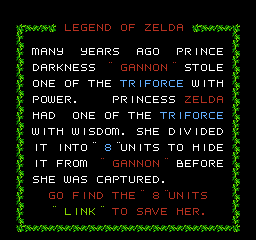
\includegraphics[width=\linewidth, height=6cm]{ch_1_1_2_zelda_1.png}
		\label{subfig:ch_1_1_2_zelda_1}
	\end{subfigure}
	\begin{subfigure}{0.49\textwidth}
		\caption{Interakcja z NPC}
		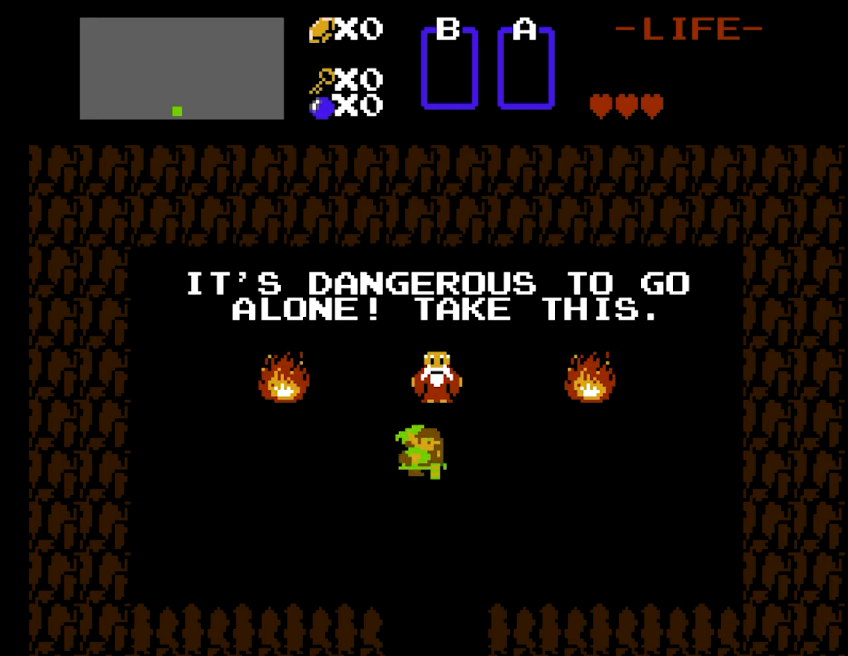
\includegraphics[width=\linewidth, height=6cm]{ch_1_1_2_zelda_2.png}
		\label{subfig:ch_1_1_2_zelda_2}
	\end{subfigure}
	\caption{The Legend of Zelda (1986)}
	\label{fig:ch1_1_2_zelda}
\end{figure}

Dekadę później gry komputerowe PC zyskały popularność dzięki tytułom jak Doom, a na rynku
pojawiły się PlayStation i Nintendo 64. Koniec XX wieku to także rozwój przenośnych gier na
fali sukcesu serii Pokemon.

Pierwszym tytułem opisanym w tej podsekcji, który operuje na perspektywie 3-osobowej jest
"Crash Bandicoot" (Rys \ref{fig:ch1_1_2_crash}). W wydanej na platformę PlayStation w 1996 roku grze
gracz steruje tytułowym Crash'em Bandicoot'em. Rozgrywkę otwiera tzw. cut-scenka (wyjaśniona również w
podsekcji \ref{subsection:ch1_2_3}), czyli krótki film wprowadzający do fabuły. To właśnie dzięki niej
gracz może usłyszeć wypowiadane imię głównego przeciwnika Crasha, doktora Neo Cortex'a.
Szalony naukowiec prowadził badania na lokalnej faunie i pragnął by Crash
stał się generałem jego armii. Crash zostaje jednak odrzucony przez maszynę do prania mózgu i ucieka
z zamku Cortex'a. Pod koniec filmu przedstawiona zostaje też "kobieta Bandicoot", na której mają zostać
przeprowadzone dalsze testy. W ten sposób gracz odkrywa dlaczego Crash przemierza kolejne poziomy (by ocalić
panią Bandicoot), dlaczego przeciwnicy są tacy a nie inni (przez testy doktora Neo Cortex'a) i co za tym
idzie kto jest jego głównym rywalem. Dodatkowo, w ramach rozgrywki mamy do czynienia z perspektywą
trójwymiarową, która jednak ulega zmianie pomiędzy poziomami. W grze występują również dwa zakończenia,
jedno wymaga perfekcyjnego przejścia gry, natomiast oba przedstawione są w formie cut-scenki.

\begin{figure}[h]
	\begin{subfigure}{0.49\textwidth}
		\caption{Cut-scenka otwierająca}
		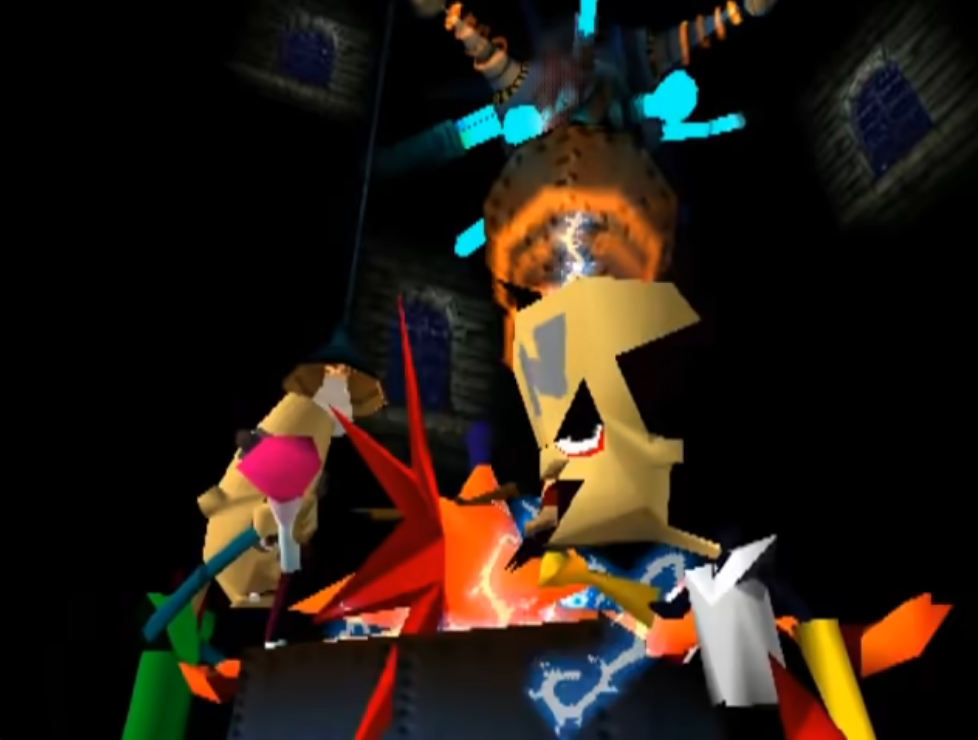
\includegraphics[width=\linewidth, height=6cm]{ch_1_1_2_crash_1.png}
		\label{subfig:ch_1_1_2_crash_1}
	\end{subfigure}
	\begin{subfigure}{0.49\textwidth}
		\caption{Crash i jego towarzysz Aku Aku}
		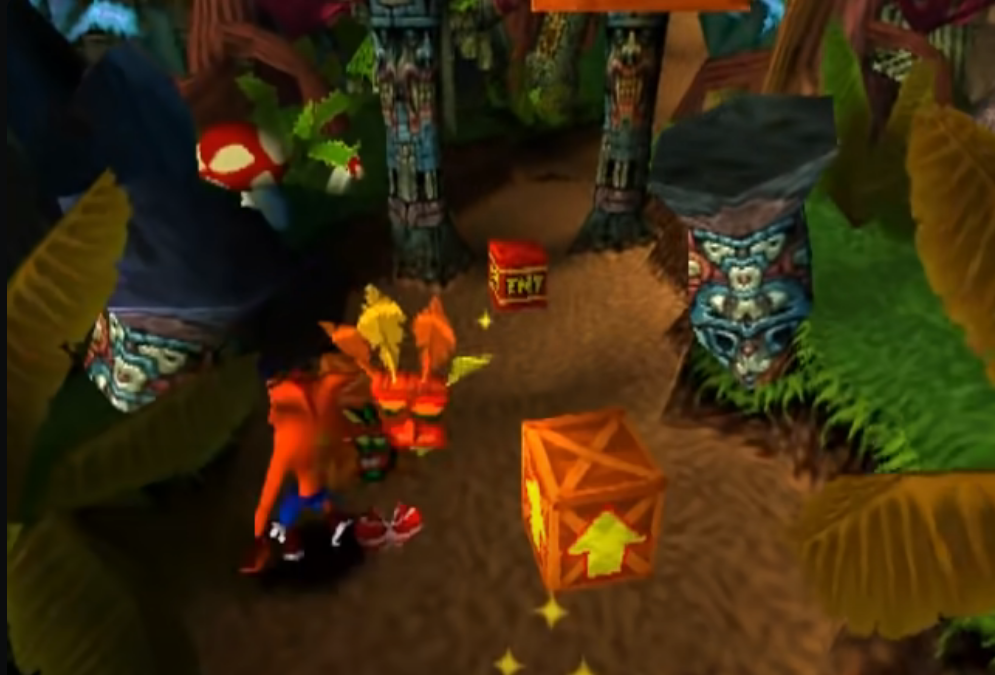
\includegraphics[width=\linewidth, height=6cm]{ch_1_1_2_crash_2.png}
		\label{subfig:ch_1_1_2_crash_2}
	\end{subfigure}
	\caption{Crash Bandicoot (1996)}
	\label{fig:ch1_1_2_crash}
\end{figure}

Uznawaną za jedną z najlepszych czy też najbardziej kultowych gier komputerowych jest
"Half-Life" (Rys \ref{fig:ch1_1_2_hl}) wydany w 1998 roku.
Wprowadzająca do rozgrywki sekwencja przedstawia najważniejsze informacje, nie zabierając
przy tym kontroli (gracz może przemieszczać się i rozglądać po kabinie pociągu). Nakreślona zostaje
postać Gordona Freemana, 27-letniego doktora fizyki teoretycznej, który pracuje w placówce Black Mesa,
położonej w Nowym Meksyku. Niemal cała warstwa fabularna zostaje wypowiedziana przez aktorów głosowych,
bez wspierających napisów. Gracz w trakcie rozgrywki spotyka różnych NPC - i to właśnie one
przekazują mu istotne informacje (posiadają również odpowiednie animacja poruszania ustami przy
wypowiadaniu kwestii). Przejścia pomiędzy poziomami są maskowane przez m.in. podróże windą czy
bardzo krótkie doczytywanie kolejnych fragmentów świata --- co sprawia, że rozgrywka pozostaje
bez przerwy imersyjna.

\begin{figure}[h]
	\begin{subfigure}{0.49\textwidth}
		\caption{NPC w monologu}
		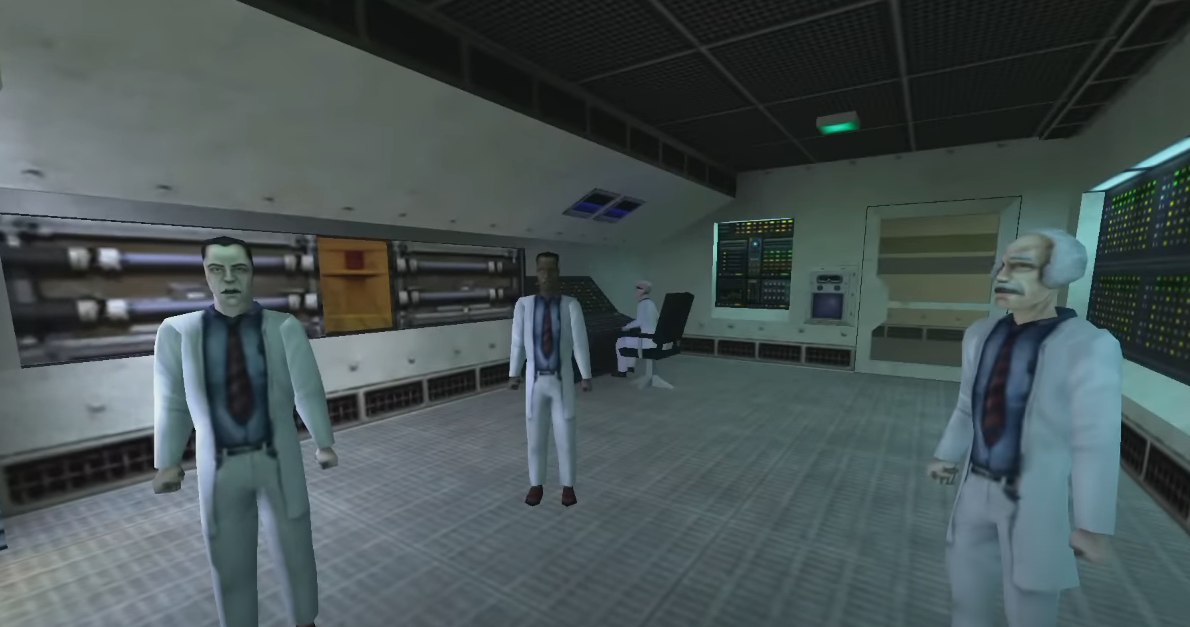
\includegraphics[width=\linewidth, height=6cm]{ch_1_1_2_hl_1.png}
		\label{subfig:ch_1_1_2_hl_1}
	\end{subfigure}
	\begin{subfigure}{0.49\textwidth}
		\caption{Napisy w sekwencji otwierającej}
		
\includegraphics[width=\linewidth, height=6cm]{ch_1_1_2_hl_2.png}
		\label{subfig:ch_1_1_2_hl_2}
	\end{subfigure}
	\caption{Half-life (1998)}
	\label{fig:ch1_1_2_hl}
\end{figure}

\newpage

Nowe millennium przyniosło dalszy rozwój branży do rozmiarów dzisiejszej potęgi, poprzez stale
pojawiające się innowacje sprzętowe i nowe przełomowe tytuły na różne platformy.

Przykładem idealnie obrazującym rozwój w podejściu do narracji jest gra "Life is Strange" (Rys \ref{fig:ch1_1_2_lis})
wydana w 2015 roku. Jest to gra przygodowa o charakterze fikcji interkatywnej (Więcej na ten temat
w podsekcji \ref{subsection:ch1_3_2}), która wydawana była w formie epizodycznej. Każdy epizod
przypominać może podział na odcinki znany z seriali telewizyjnych czy też akty w literaturze.
Centralną postacią jest Maxine Caulfield, która odkrywa że potrafi cofnąć czas. Całość fabuły opiera się
na motywie \textit{efektu motyla}, gdzie podejmowane decyzje mogą rzutować na wydarzenia w przyszłości czy
też na relacje pomiędzy postaciami. Z tego powodu narrację można zakwalifikować jako rozgałęziającą się
(Patrz \ref{subsection:ch1_2_1}) i zarazem stanowi ona kluczowy element rozgrywki a nie tylko
"imersyjny dodatek" do niej. System dialogów zaprezentowany w "Life is Strange" oparty jest na popularnej
strukturze kołowej (Patrz \ref{subsection:ch1_3_1}) z motywem drzewa, tzn. konkretne wybory dialogowe
wiążą się z gamą zupełnie nowych wyborów w dalszej części rozmowy (mechanika cofania czasu pozwala
graczowi rozgrywać dialog na inny sposób).

\begin{figure}[h]
	\begin{subfigure}{0.49\textwidth}
		\caption{Wybór z ostrzeżeniem o konsekwencjach}
		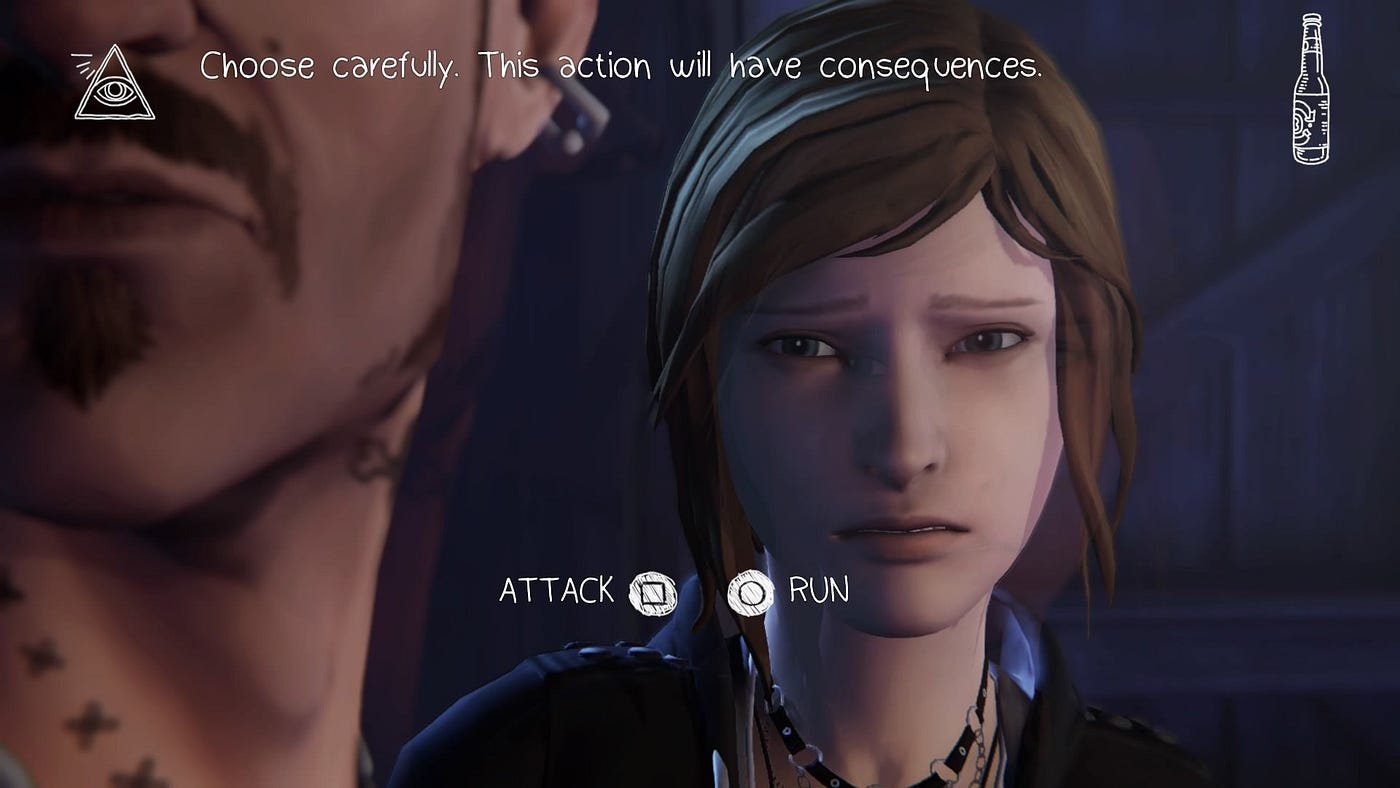
\includegraphics[width=\linewidth, height=6cm]{ch_1_1_2_lis_1.png}
		\label{subfig:ch_1_1_2_lis_1}
	\end{subfigure}
	\begin{subfigure}{0.49\textwidth}
		\caption{System dialogowy kołowy}
		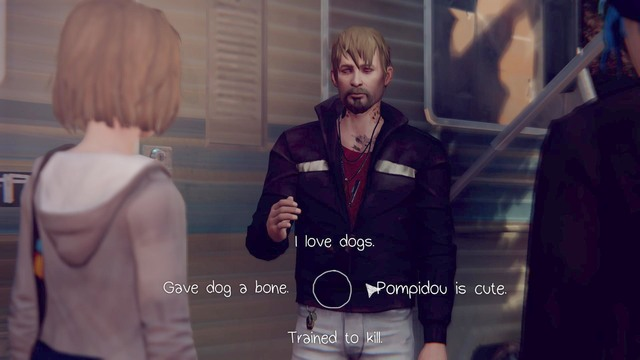
\includegraphics[width=\linewidth, height=6cm]{ch_1_1_2_lis_2.png}
		\label{subfig:ch_1_1_2_lis_2}
	\end{subfigure}
	\caption{Life is Strange (2015)}
	\label{fig:ch1_1_2_lis}
\end{figure}

\newpage

Jako wzór gry z otwartym światem niewątpliwie można uznać tytuł "Wiedźmin 3" (Rys \ref{fig:ch1_1_2_witcher})
wydane w 2015 roku i wyprodukowane przez polskie studio CD Projekt Red. Akcja rozgrywka się w świecie
opartym na powieściach i opowiadaniach Andrzeja Sapkowskiego a gracz wciela się w rolę Geralta z Rivii.
Forma otwartego świata oznacza w tym przypadku tyle, że grający ma możliwość swobodnego poruszania się
po krainach i jest też w stanie podejmować się różnych zadań w "niemal" dowolnej kolejności. Sprawia to, że
gracz nie czuje się niczym aktor odgrywający kolejne sceny a za to jest reżyserem własnych przygód.
System dialogowy zorganizowany jest w formę menu wyborów, przy czym na niektóre zdarzenia gracz ma
ograniczony czas odpowiedzi (Przedstawione na Rys. \ref{subfig:ch_1_1_2_witcher_2}). Dodatkowo, niektóre
opcje mogą wymagać posiadania określonej ilości pieniędzy czy też odblokowania określonych umiejętności.

\begin{figure}[h]
	\begin{subfigure}{0.49\textwidth}
		\caption{Mapa świata (żółte punkty - zadania)}
		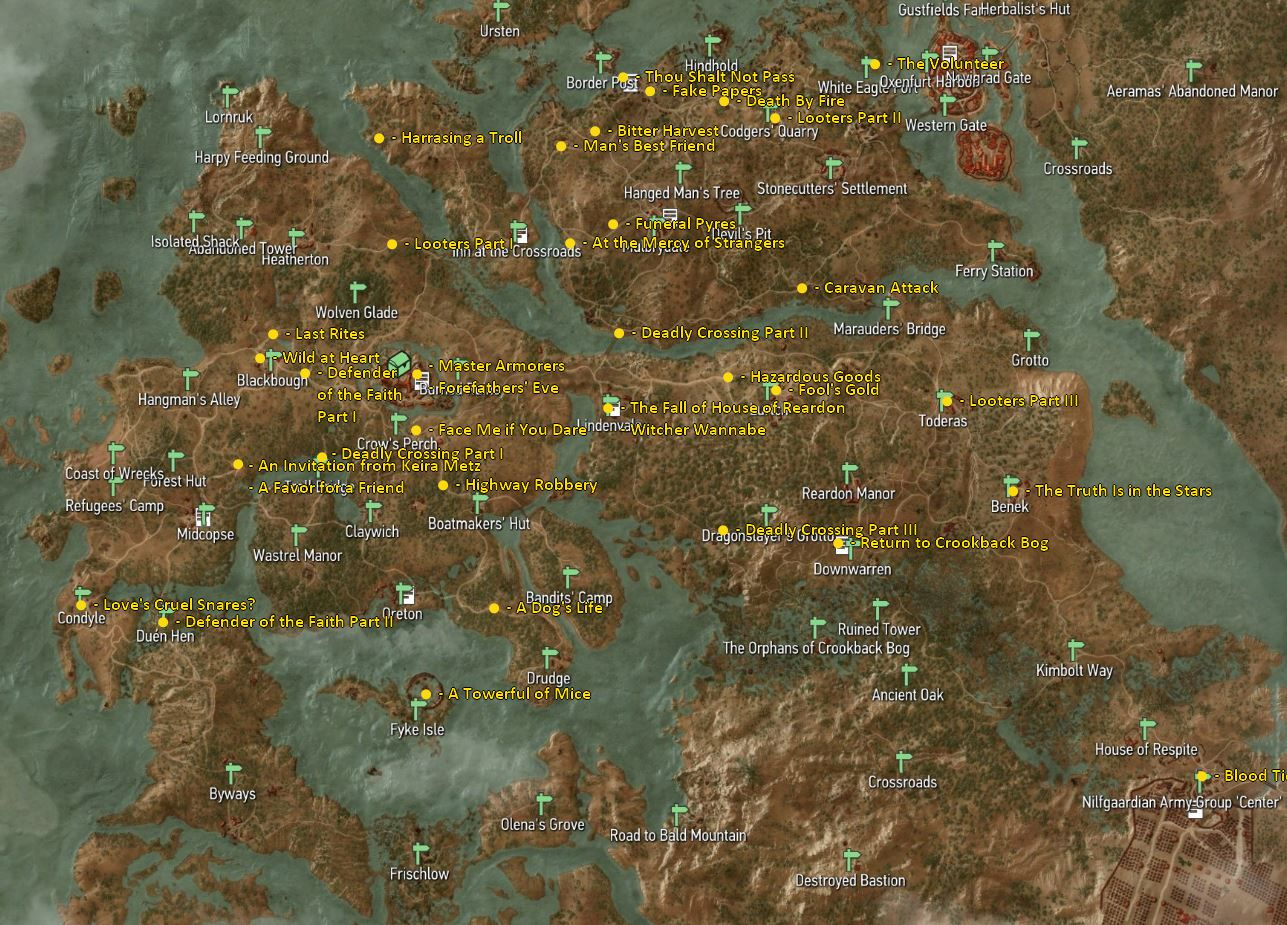
\includegraphics[width=\linewidth, height=6cm]{ch_1_1_2_witcher_1.png}
		\label{subfig:ch_1_1_2_witcher_1}
	\end{subfigure}
	\begin{subfigure}{0.49\textwidth}
		\caption{Dialog z czasem na decyzję}
		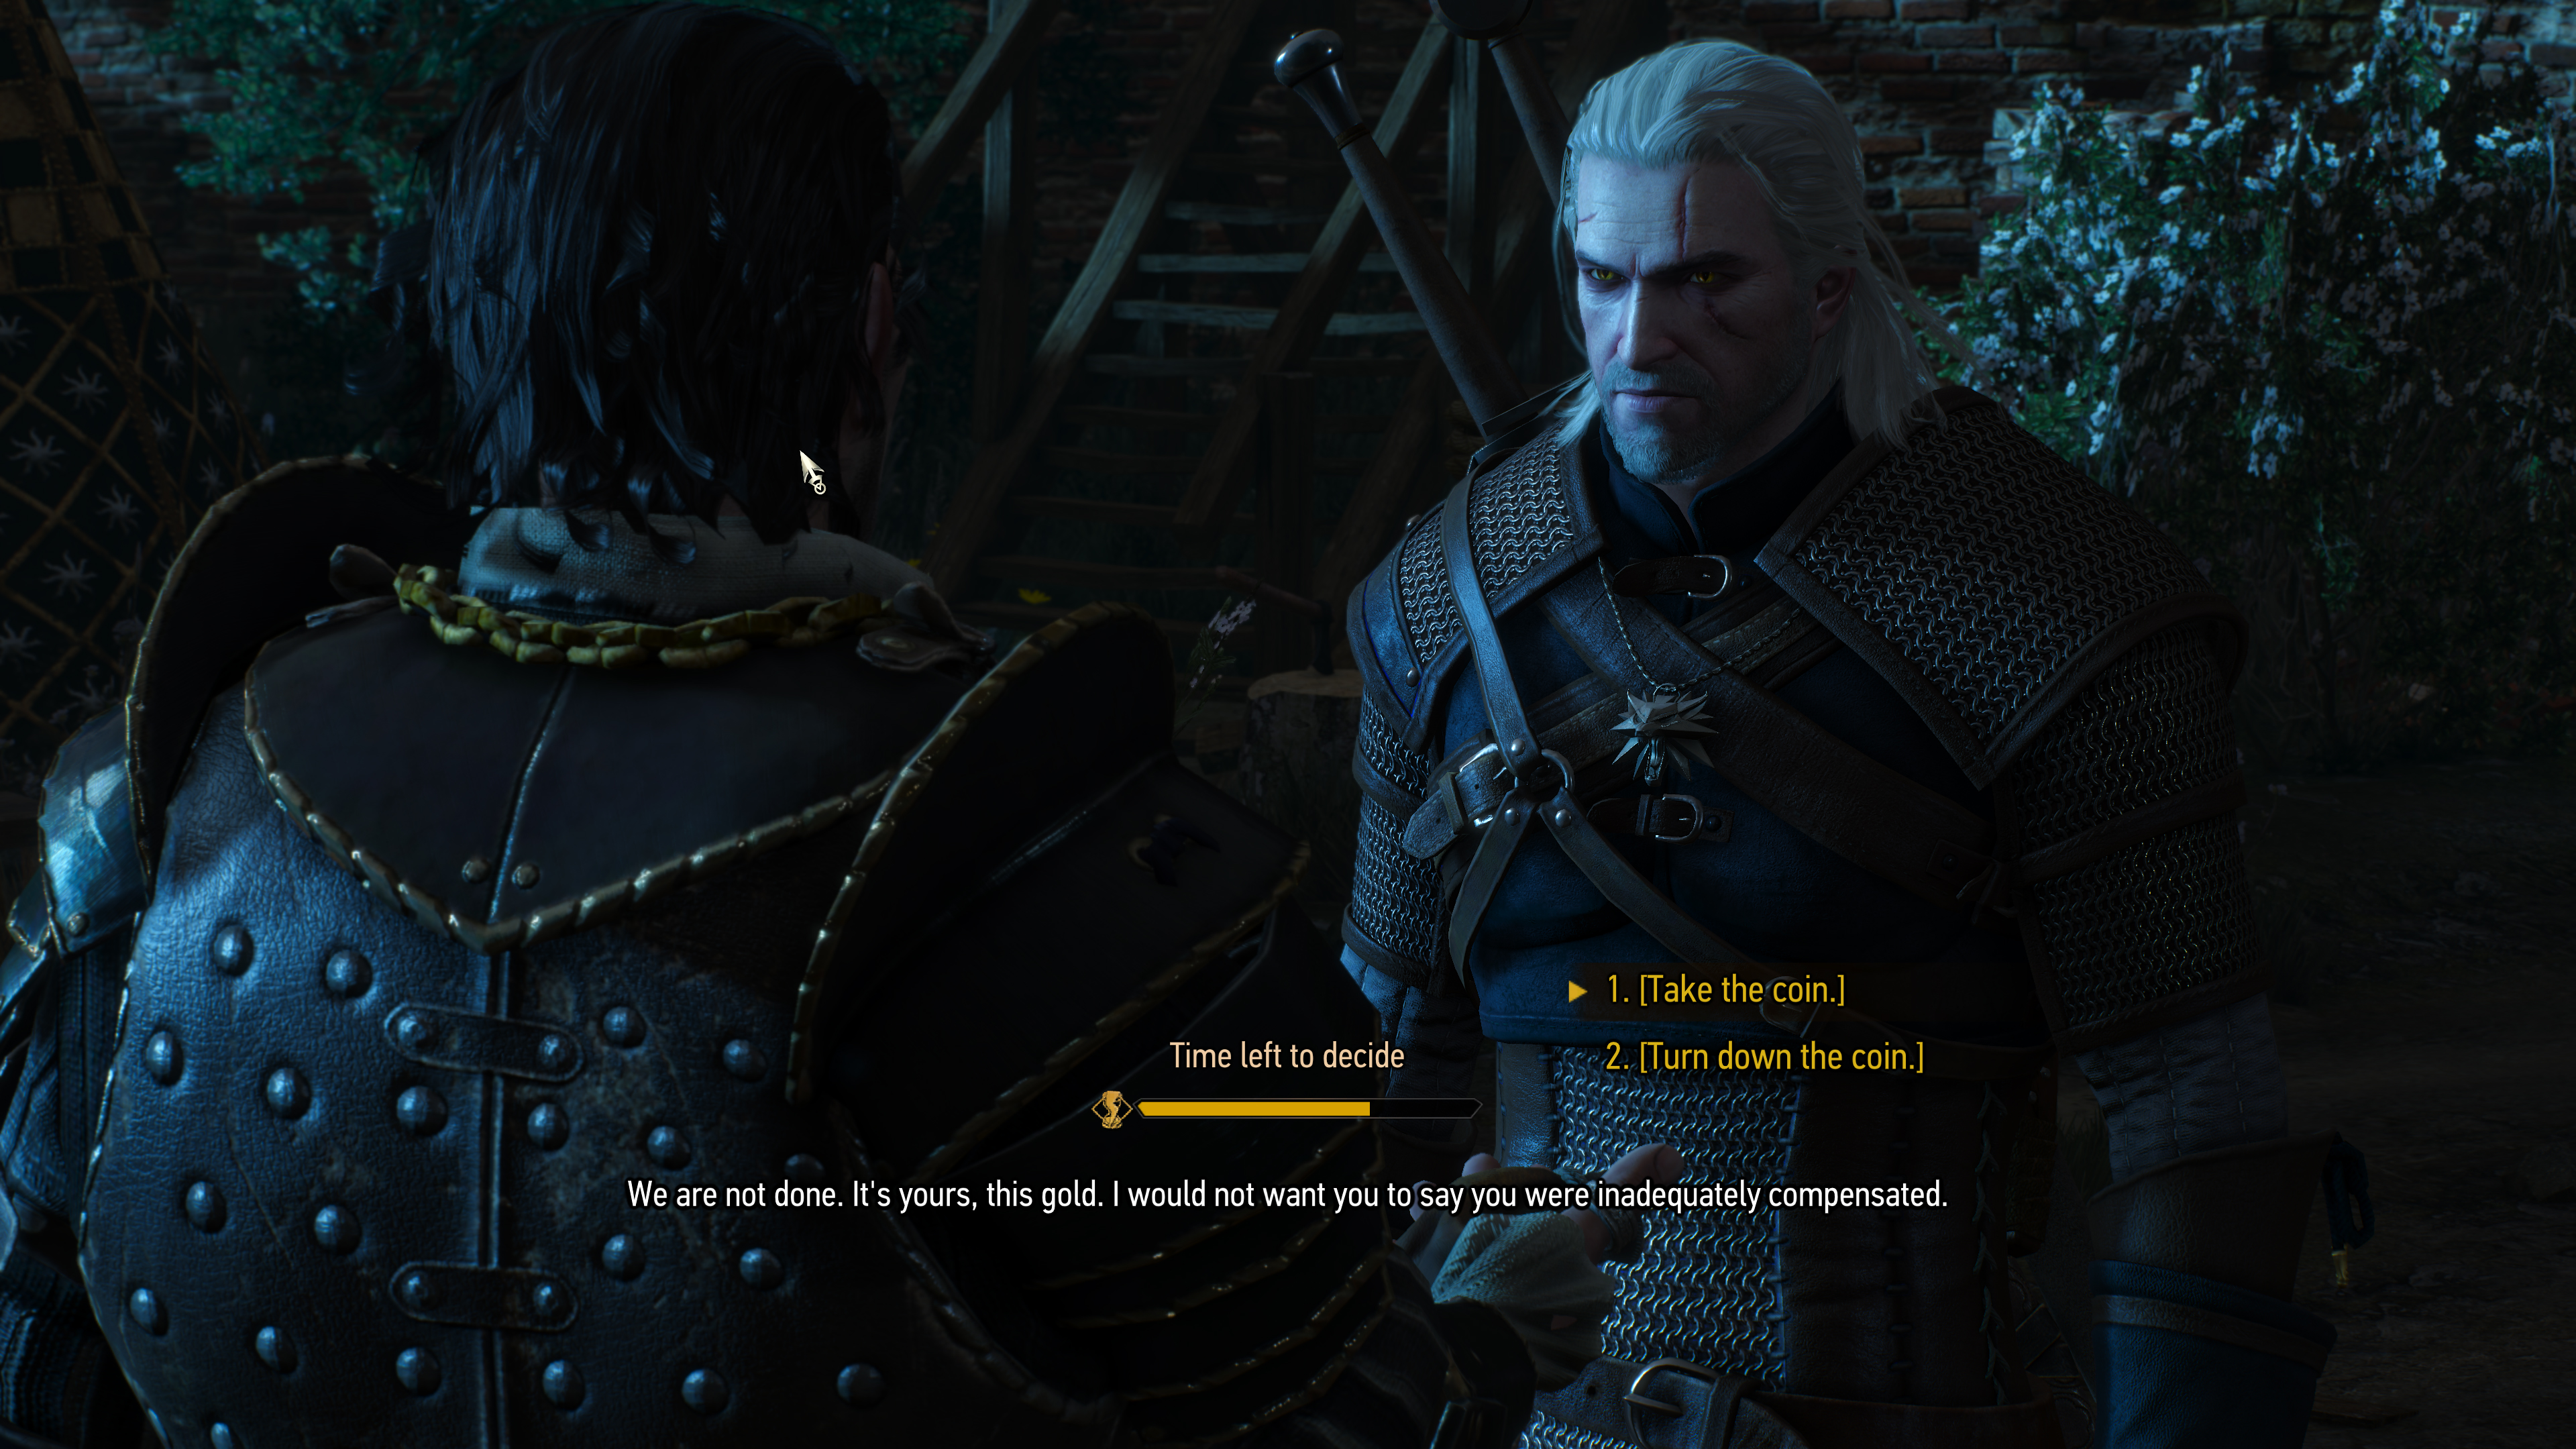
\includegraphics[width=\linewidth, height=6cm]{ch_1_1_2_witcher_2.png}
		\label{subfig:ch_1_1_2_witcher_2}
	\end{subfigure}
	\caption{Wiedźmin 3 (2015)}
	\label{fig:ch1_1_2_witcher}
\end{figure}

\newpage

\subsection{Prześledzenie rozwoju narracji na przykładzie serii Final Fantasy}\label{subsection:ch1_1_3}

% TL;DR:
% - Od FF1 zasadniczo nieme postacie, 2D pikseloza, tylko tekstowe monologi od NPC, cut-scenki bardzo
% prowizoryczne na zasadzie ruszania kamerą w grze. Zero voice actingu i fabuły postaci.
% - Od FF7 pełno-prawna cut-scenka otwarcia, 3D widok, no i chyba bardziej nastawienie na postacie
% - Od FF10 bardzo dużo przerywników filmowych, nastawienie na dialogi, voice acting
% - FF13 historia zeszła na bok w formie dzienniczków, głównie chodzi o dialogi i postacie
% - FF15 jest open world'owe i odeszli od JRPG na rzecz gry akcji

Seria "Final Fantasy" zadebiutowała w 1987 roku na konsoli NES, a samym twórcą gry był Hironobu
Sakaguchi. Na przestrzeni kolejnych lat powstało 14 numerowanych odsłon serii oraz wiele spin-offów
\cite{the_evolution_of_final_fantasy}. W głównej serii każda gra nie miała nic wspólnego z poprzednią
pod względem fabuły, postaci czy uniwersum. Pojawiały się wspólne motywy i stworzenia, ale na ogół
każde "Final Fantasy" stanowiła odrębną, zamkniętą przygodę\cite{the_evolution_of_final_fantasy}.

Seria przeżywała i nadal przeżywa swoistego rodzaju ewolucję narracyjną. Elementy, które stanowiły
główną część fabularną, zeszły na dalszy plan. Początkowo mało istotni bezimienni protagoniści zostali
zastąpieni przez postacie angażujące się w dialogi i rozwijające się na przestrzeni gry
\cite{the_evolution_of_final_fantasy}.

Aby prześledzić proces zmian w serii, dokonany zostanie przegląd kolejnych odsłon "Final Fantasy" na
podstawie informacji zebranych przez Kevin'a Kryah\cite{the_evolution_of_final_fantasy} oraz
Hayes'a Madsen'a\cite{25_years_later}.

W pierwszej odsłonie (Rys. \ref{fig:ch1_1_3_ff1}) fabuła była dość prosta - czterech sterowalnych
bohaterów, znanych jako \textit{Wojownicy Światła}, przybywają do królestwa \textit{Cornelia}, niosąc
mistyczne kule. Zostają poinformowani, że muszą pokonać cztery żywioły, by przywrócić światu równowagę
\cite{the_evolution_of_final_fantasy}. W samej grze \textit{Wojownicy Światła} są niemymi postaciami,
natomiast występują NPC (ang. \textit{non-playable character}), którzy w formie monologów przekazują
graczowi informacje. Monologi te przedstawione są jedynie w formie tekstowej, nie występuje bowiem
zjawisko aktorstwa głosowego (po ang. \textit{voice acting}). Cut-scenki (patrz \ref{subsection:ch1_2_3})
są bardzo prymitywne, na zasadzie poruszania kamerą i wykorzystaniu animacji występujących w grze
(nie są prerenderowane). W ramach ekranu startowego gry przedstawione zostaje graczowi krótkie
wprowadzenie fabularne (Rys. \ref{subfig:ch_1_1_3_ff1_1}).

\begin{figure}[h]
	\begin{subfigure}{0.49\textwidth}
		\caption{Ekran wprowadzający}
		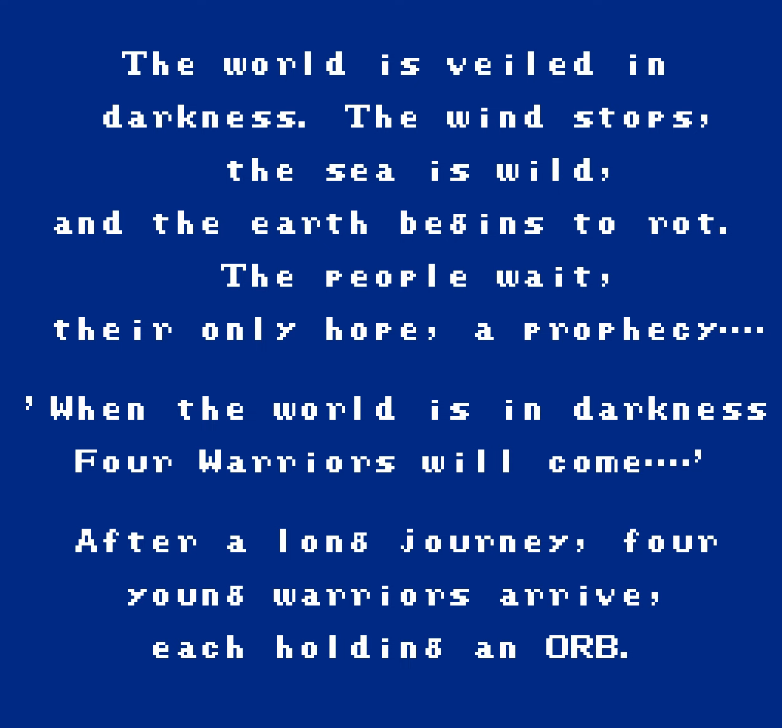
\includegraphics[width=\linewidth, height=6cm]{ch_1_1_3_ff1_1.png}
		\label{subfig:ch_1_1_3_ff1_1}
	\end{subfigure}
	\begin{subfigure}{0.49\textwidth}
		\caption{Rozmowa z NPC}
		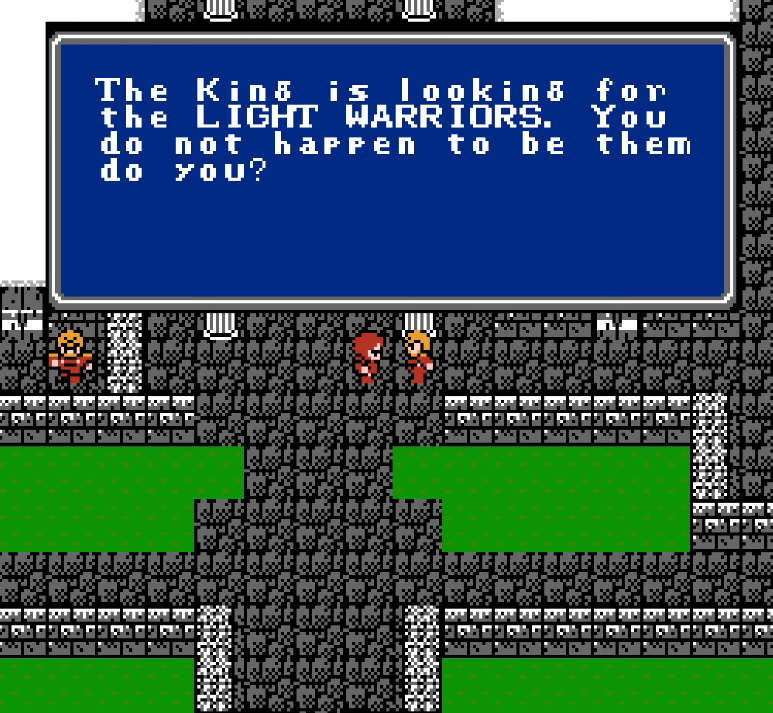
\includegraphics[width=\linewidth, height=6cm]{ch_1_1_3_ff1_2.png}
		\label{subfig:ch_1_1_3_ff1_2}
	\end{subfigure}
	\caption{Final Fantasy I (1987)}
	\label{fig:ch1_1_3_ff1}
\end{figure}

\newpage

Żadne z kolejnych "Final Fantasy" nie wniosły zbyt wiele pod względem złożoności fabuły. "Final Fantasy
IV" wprowadziła większy nacisk na rozwój postaci poprzez cut-scenki i wątki bohaterów. Głównym elementem
nadal pozostawała walka z "ostatecznym złowrogim bossem", lecz przy okazji gracz był w stanie poznać
główne postacie\cite{the_evolution_of_final_fantasy}.

"Final Fantasy VI" poszła o krok dalej - rola postaci zaczęła przesłaniać nadrzędną fabułę. Sceny takie
jak próba samobójcza Celes czy rzut monetą między Edgarem i Sabinem niewiele wniosły do głównego wątku,
ale dobrze charakteryzowały bohaterów w sposób, którego nie sposób opisać samymi dialogami.
\cite{the_evolution_of_final_fantasy}.

W ramach "Final Fantasy VII" (Rys. \ref{fig:ch1_1_3_ff7}) doszło do przełomu graficznego, ponieważ
rozgrywka odbywała się w świecie trójwymiarowym. Dodatkowo, ta część okraszona została pełnoprawną
cut-scenką otwierającą.

"Final Fantasy VII" i VIII kontynuowały trend nastawienia na postaci.
Ich losy stały się głównym tematem, a walka dobra ze złem została odstawiona na dalszy plan.
"Final Fantasy VIII" wydawała się wręcz niezainteresowana głównym wątkiem, a jej zakończenie
koncentrowało się na zamknięciu wątków postaci i zostało zwieńczone pocałunkiem na balkonie
\cite{the_evolution_of_final_fantasy}.

W swej istocie, "Final Fantasy VIII" jest formą opowieści miłosnej. Mimo występowania oczywistych
elementów fantastycznych czy fikcyjnych, to głównym motywem przyciągającym uwagę gracza jest
miłość Squalla i Rinoi\cite{25_years_later}.

Hayes Madsen sugeruje, iż to właśnie przez występowanie takich osobistych historii czy relacji między
postaciami fabuła "Final Fantasy VIII" jest tak często wspominana. Twórcy przedstawili bowiem występujące
pomiędzy głównymi postaciami poczucie koleżeństwa i ich wspólnego rozwoju\cite{25_years_later}.

\begin{figure}[h]
	\begin{subfigure}{0.49\textwidth}
		\caption{Klatka cut-scenki wprowadzającej}
		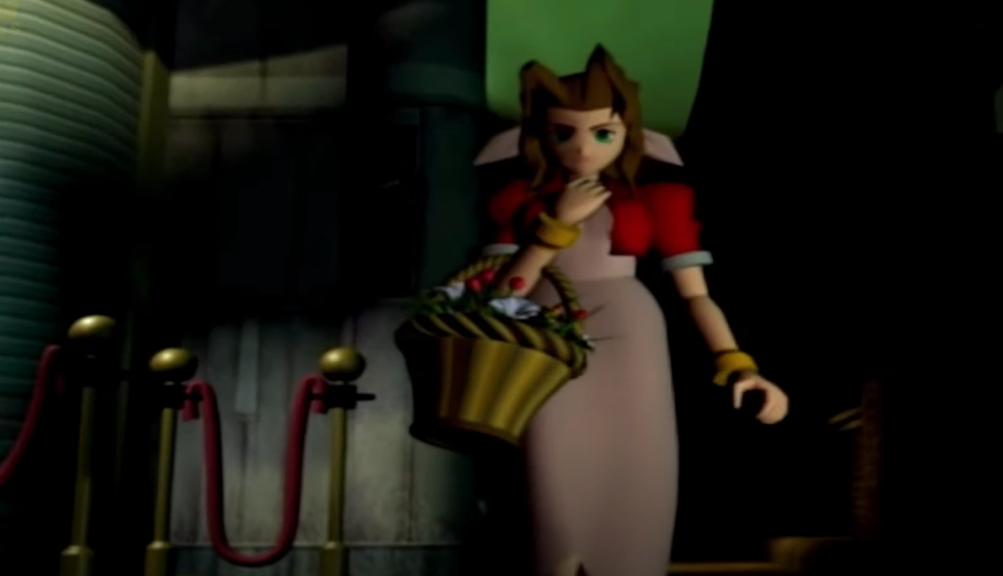
\includegraphics[width=\linewidth, height=6cm]{ch_1_1_3_ff7_1.png}
		\label{subfig:ch_1_1_3_ff7_1}
	\end{subfigure}
	\begin{subfigure}{0.49\textwidth}
		\caption{Dialogi pomiędzy postaciami}
		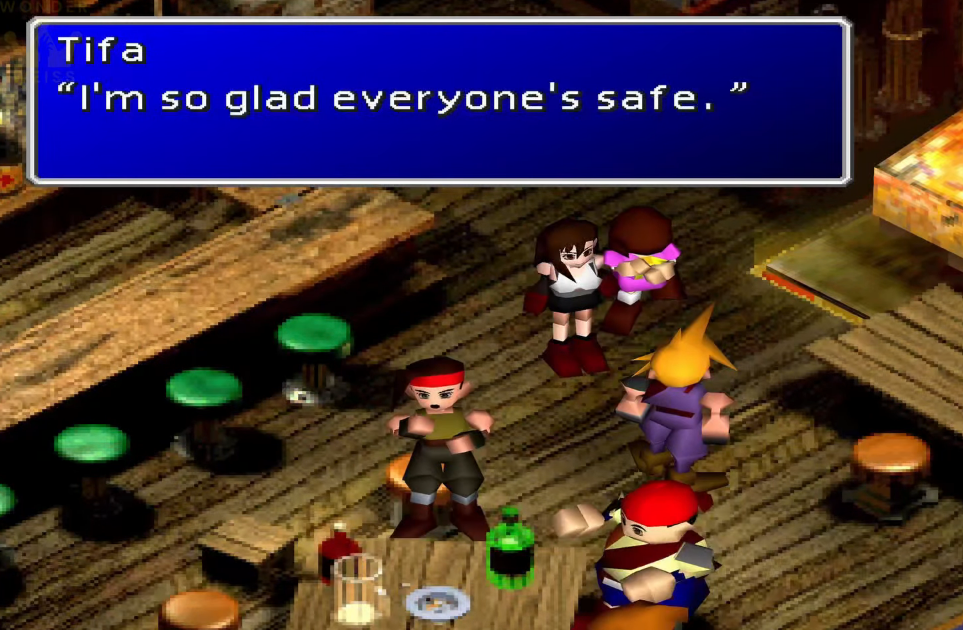
\includegraphics[width=\linewidth, height=6cm]{ch_1_1_3_ff7_2.png}
		\label{subfig:ch_1_1_3_ff7_2}
	\end{subfigure}
	\caption{Final Fantasy VII (1997)}
	\label{fig:ch1_1_3_ff7}
\end{figure}

\newpage

Gdy seria wkroczyła w XXI wiek, gry oddalały się jeszcze bardziej od swych korzeni. "Final Fantasy
IX" kontynuowała nastawienie na postacie, dodając klimat europejskich baśni czy aluzji do Szekspira i
Carrolla. "Final Fantasy X" (Rys. \ref{fig:ch1_1_3_ff10}) podejmowała tematy religii i człowieczeństwa,
prezentując jednocześnie jedne z najbardziej artystycznych wizji w serii\cite{the_evolution_of_final_fantasy}.
Rozgrywka została urozmaicona bardzo wieloma zaawansowanymi przerywnikami filmowymi. Postacie wydawać się
mogą zdecydowanie bardziej realistyczne czy "żywsze" ze względu na udział aktorów głosowych, począwszy
od tej części.

\begin{figure}[h]
	\begin{subfigure}{0.49\textwidth}
		\caption{Cut-scenka z gry}
		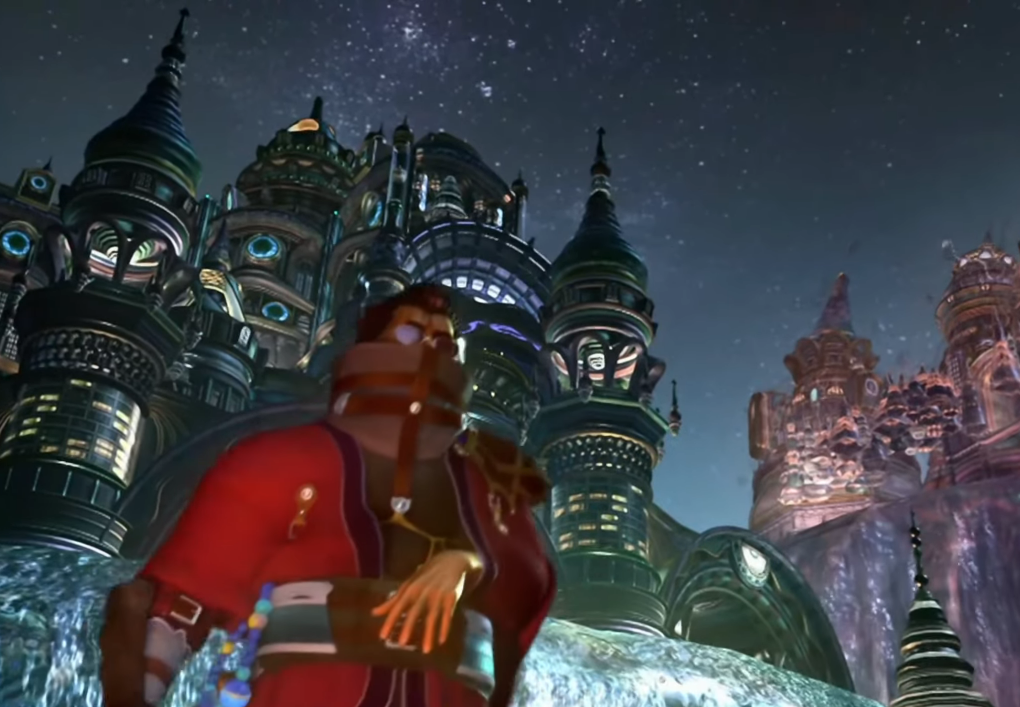
\includegraphics[width=\linewidth, height=6cm]{ch_1_1_3_ff10_1.png}
		\label{subfig:ch_1_1_3_ff10_1}
	\end{subfigure}
	\begin{subfigure}{0.49\textwidth}
		\caption{Dialogi pomiędzy postaciami}
		
\includegraphics[width=\linewidth, height=6cm]{ch_1_1_3_ff10_2.png}
		\label{subfig:ch_1_1_3_ff10_2}
	\end{subfigure}
	\caption{Final Fantasy X (2001)}
	\label{fig:ch1_1_3_ff10}
\end{figure}

\newpage

"Final Fantasy XIII" (Rys. \ref{fig:ch1_1_3_ff13}) w pełni skupiło się na rozwoju postaci i
formie wizualnej, natomiast sensowność fabuły pozostawiała wiele do życzenia. W rzeczywistości większość
istotnych informacji nie jest dostarczana w dialogach, ale za pośrednictwem wpisów do dziennika,
znajdywanych przez gracza w trakcie rozgrywki. To raczej postacie zajęły centralne miejsce, a
bezsensowna fabuła starała się jedynie związać ze sobą wszystkie wątki
bohaterów\cite{the_evolution_of_final_fantasy}.

\begin{figure}[h]
	\begin{subfigure}{0.49\textwidth}
		\caption{zzz}
		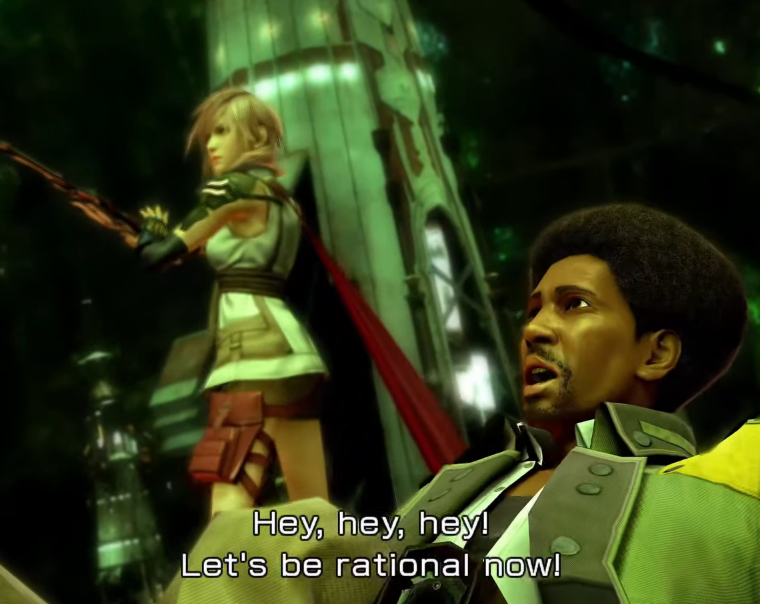
\includegraphics[width=\linewidth, height=6cm]{ch_1_1_3_ff13_1.png}
		\label{subfig:ch_1_1_3_ff13_1}
	\end{subfigure}
	\begin{subfigure}{0.49\textwidth}
		\caption{zzz}
		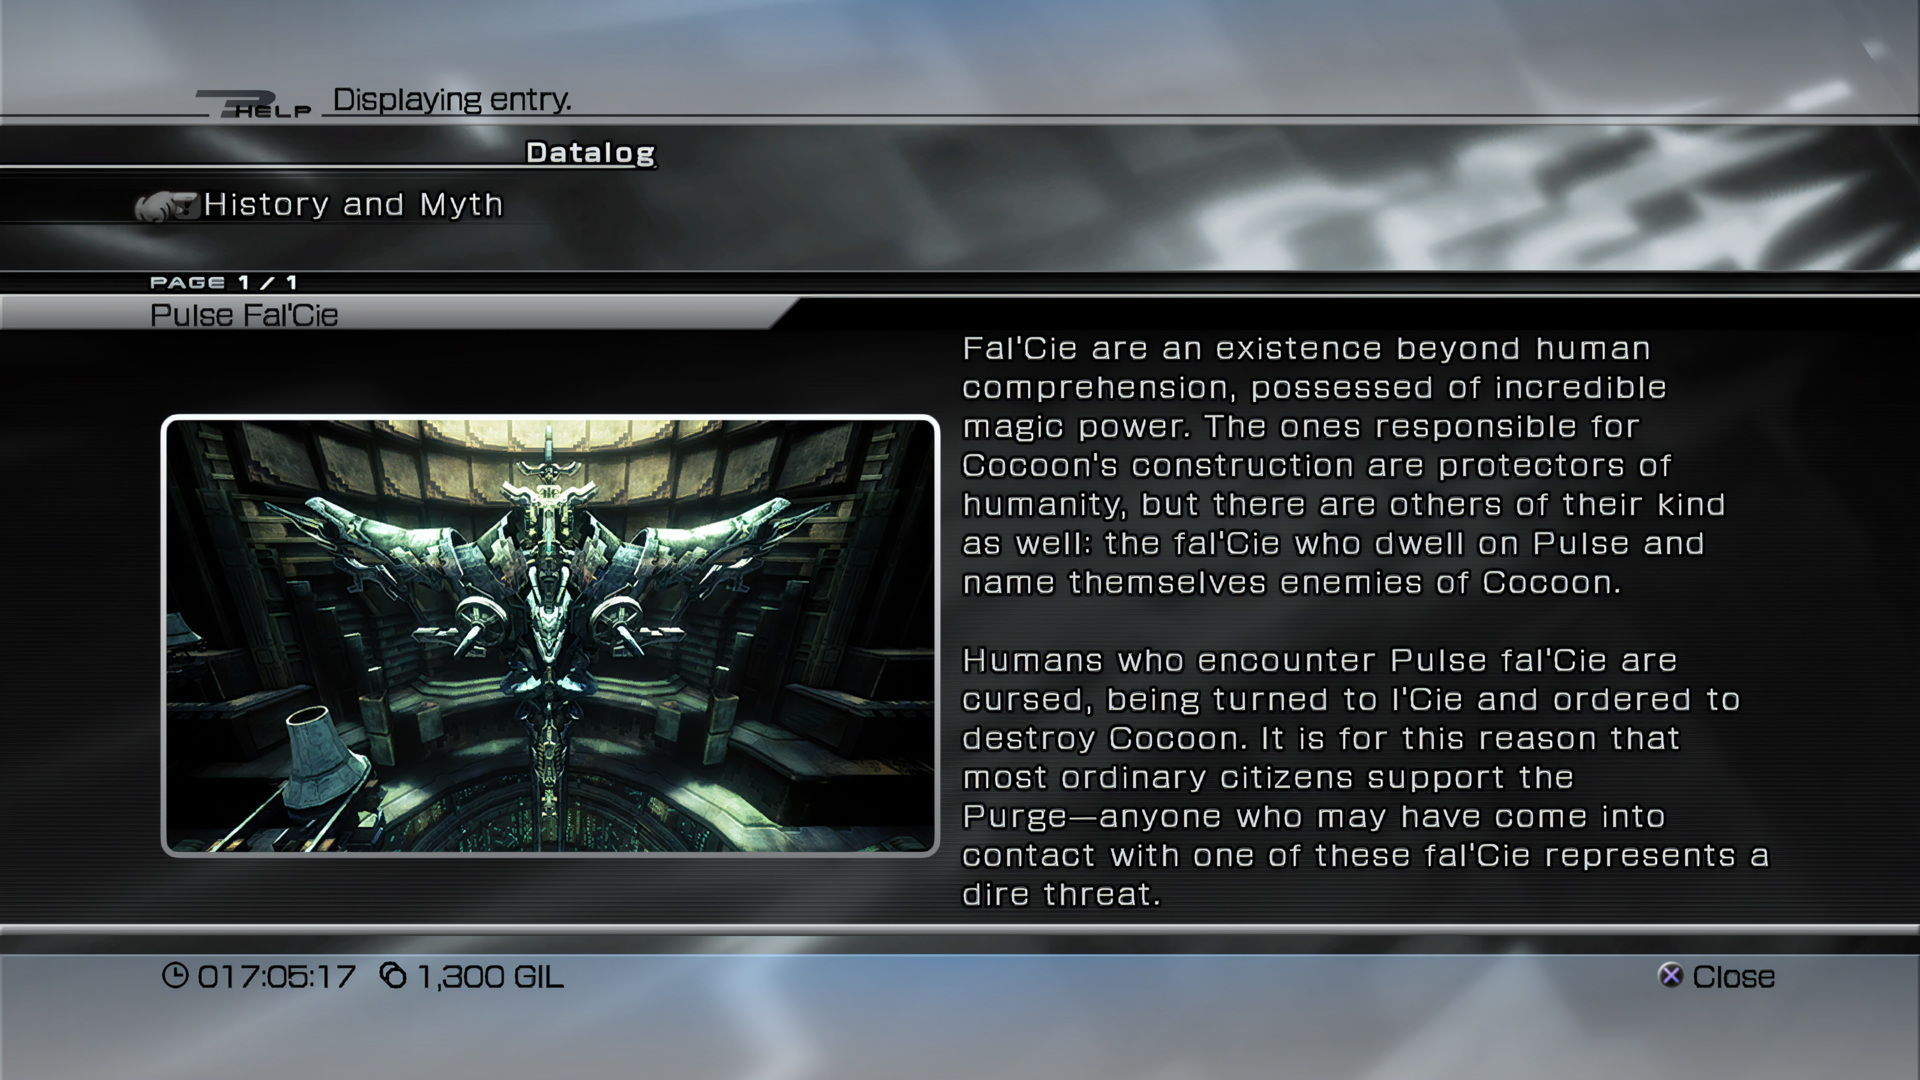
\includegraphics[width=\linewidth, height=6cm]{ch_1_1_3_ff13_2.png}
		\label{subfig:ch_1_1_3_ff13_2}
	\end{subfigure}
	\caption{Final Fantasy XIII (2009)}
	\label{fig:ch1_1_3_ff13}
\end{figure}

Seria "Final Fantasy" rozwija się po dzień dzisiejszy, a twórcy nadal próbują używać różnych rozwiązań by
wyróżnić kolejne tytuły. Przykładowo, w najnowszej odsłonie serii --- "Final Fantasy XV" --- deweloperzy
odeszli od konwencji JRPG (ang. \textit{Japanese role-playing game}) na rzecz gry akcji z otwartym światem.

Na przestrzeni lat seria "Final Fantasy" przeszła znaczącą ewolucję pod względem roli i znaczenia narracji.
Niezależnie od zmian w strukturze rozgrywki czy sposobie prezentowania fabuły, widoczny jest stale rosnący
wpływ elementów narracyjnych na całokształt kolejnych odsłon serii.

\section{Rodzaje narracji w grach komputerowych}\label{section:ch1_2}

Super wiele gierek wykorzystuje bardzo dużo technik itp do przedstawiania narracji, w tej sekcji
wymienione zostaną najważniejsze z nich.

\subsection{Struktury narracji}\label{subsection:ch1_2_1}

Struktura narracji to w ramach tej pracy uporządkowanie kolejnych wydarzeń I guess.

\subsubsection*{Liniowa}

ggggggggggggg

\subsubsection*{Łańcuch pereł}

ggggggggggggg

\subsubsection*{Rozgałęziająca się}

gggggggggggggg

\subsubsection*{Park rozrywki}

gggggggggggggg

\subsubsection*{Cegiełki}

gggggggggggg

\subsection{Techniki przedstawienia narracji}\label{subsection:ch1_2_2}

No ogólnie narrację można przedstawiać na różne sposoby wiadomo mhm mhm...

\section{Systemy dialogowe w grach komputerowych}\label{section:ch1_3}

fefef

\subsection{Popularne systemy dialogowe}\label{subsection:ch1_3_1}

fefef

\subsection{Interaktywna fikcja - system poleceń}\label{subsection:ch1_3_2}

ortatraoitrmoi
\graphicspath{{chapters/chapter2/imgs/}}

\chapter{Rodzaje narracji w grach komputerowych}\label{section:ch1_2}

Poniższa sekcja ma na celu uporządkowanie --- znanych z literatury czy też istniejących
przykładów --- struktur narracyjnych, za pomocą których opisać można sekwencję kolejnych
wydarzeń w grze. Dodatkowo, przedstawione zostaną kluczowe sposoby czy też techniki, za
pomocą których twórcy budują wirtualne światy fabularne.

\section{Struktury narracyjne}\label{subsection:ch1_2_1}

Pod pojęciem \textit{struktury narracyjnej} rozumiane jest \textbf{uporządkowanie}
wydarzeń odbywających się w grze, które niosą jakiekolwiek przesłanki fabularne.
Nie oznacza to, że każde wydarzenie musi się odbyć --- może być to bowiem zależne od
decyzji podjętych przez grającego. Wyszczególnione zostaną trzy klasyczne struktury,
które zapewniają dość płynny przebieg historii, a są to: \textit{liniowa}, \textit{łańcuch pereł},
\textit{rozgałęziającą się}\cite{the_evolution_of_video_games}\cite{theorising_narrative}\cite{narrative_structures}.
Z zakresu mniej oczywistych architektur dodatkowo warto wspomnieć o modelach
\textit{parku rozrywki} i \textit{cegiełek}\cite{theorising_narrative}.

\subsection{Liniowa}

Jest to forma przekazu znana bardzo dobrze z literatury czy też kinematografii. Sprowadza się ona
bowiem do jednego ciągu zdarzeń, gdzie odbiorca nie ma wpływu na dalszy przebieg fabuły lecz jest
on raczej pasywnym obserwatorem odgrywających się scen. W przypadku książki czy filmu jest to
naturalne podejście ze względu na brak interaktywności. Jeśli chodzi o gry komputerowe, to
strukturę tą można zaobserwować zwłaszcza w \textit{"starszych"} tytułach (Np. wspomniany wcześniej
"Crash Bandicoot" - patrz \ref{subsection:ch1_2}). Gra zasadniczo może być ukończona na jeden
sposób --- tak jak to zaplanowali projektanci\cite{the_evolution_of_video_games} (Patrz Rys. \ref{fig:ch1_2_1_linear}).

\begin{figure}[h]
    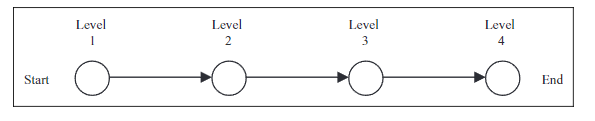
\includegraphics[width=\textwidth]{ch2_1_linear.png}
    \caption{Liniowa struktura gry\cite{narrative_structures}}
    \centering
    \label{fig:ch1_2_1_linear}
\end{figure}

\subsection{Łańcuch pereł}

W ramach tego modelu gracze uzyskują pewnego rodzaju \textit{"iluzję"} wyboru. Występują podczas
rozgrywki momenty swobody, gdzie grający mają poczucie wpływu na dalszy przebieg fabularny. W
rzeczywistości jednak podejmowane przez nich decyzje mogą nie posuwać historii na przód, a same
postępy narracyjne nadal znajdują się pod kontrolą projektantów gry\cite{theorising_narrative}.
Tak jak przedstawiono na rysunku \ref{fig:ch1_2_1_pearls} --- mogą występować tymczasowe rozgałęzienia
wychodzące od głównej sekwencji fabularnej, natomiast zostają one w końcu urwane, a gracz zobowiązany
jest do kontynuowania przygody według zaplanowanej historii. Jako przykład może służyć "The Legend
of Zelda" (Patrz \ref{subsection:ch1_2}), gdzie grający może zwiedzać dane poziomy w dość dowolny
sposób, natomiast musi ostatecznie trafić na główną ścieżkę by móc dokonać postępu.

\begin{figure}[h]
    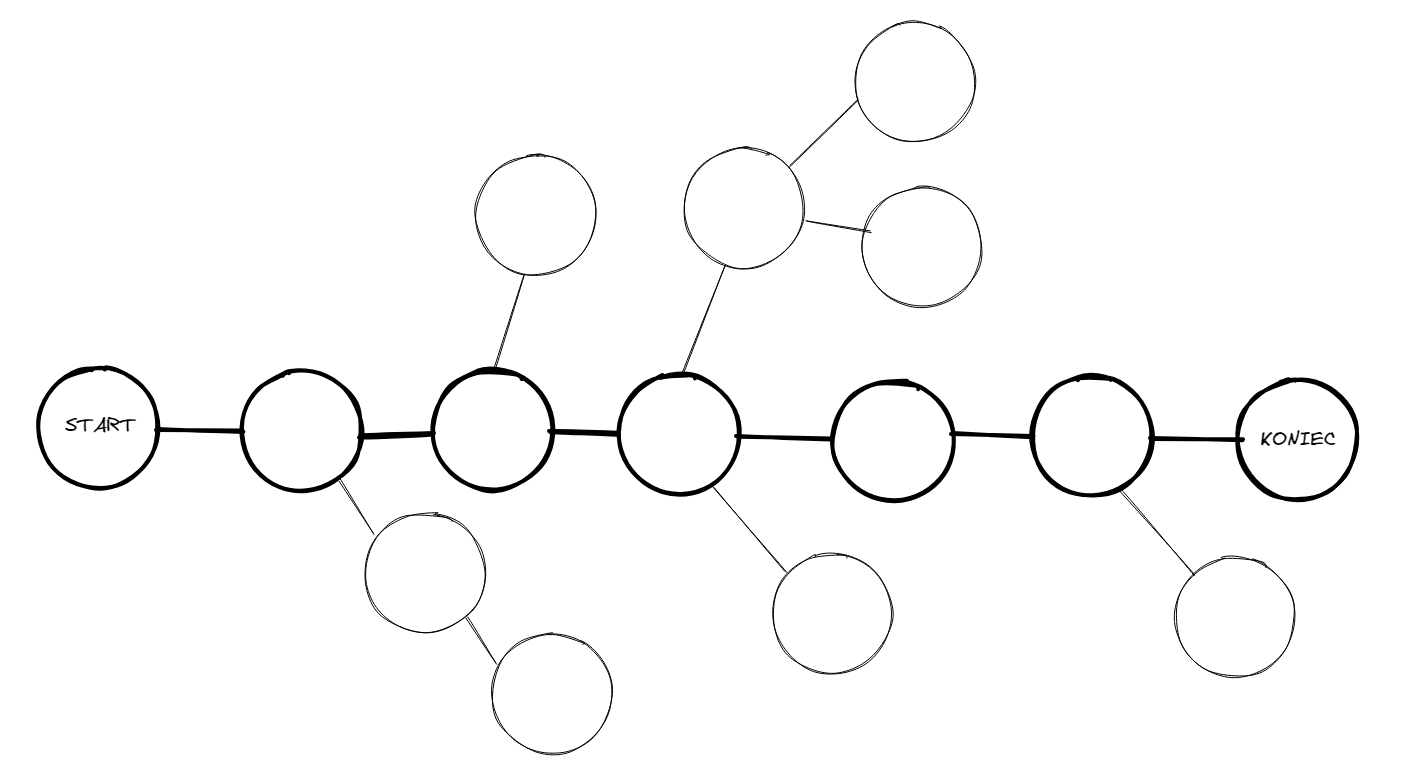
\includegraphics[width=\textwidth]{ch2_1_pearls.png}
    \caption{Struktura łańcuchu pereł}
    \centering
    \label{fig:ch1_2_1_pearls}
\end{figure}

\subsection{Rozgałęziająca się}

Metodą, która oferuje graczowi istotny wpływ na przebieg dalszej rozgrywki jest zdecydowanie
model rozgałęziający się. Jak sama nazwa wskazuje, historia nie trzyma się jednej konkretnej wersji
lecz jest w stanie \textit{"rozgałęziać się"} w wielu innych możliwych kierunkach. Może to wynikać
z jawnych decyzji podejmowanych przez gracza w istotnych momentach lub też ze względu na sposób
w jaki podchodzi on do rozgrywki (np. może pomijać pewne elementy świata)\cite{theorising_narrative}.
W wyniku takich rozgałęzień wytwarza się pewnego rodzaju "sieć możliwości fabularnych"\cite{theorising_narrative}
--- które z reguły muszą być uprzednio przygotowane przez projektantów gry. Struktura ta została
przedstawiona na rysunku \ref{fig:ch1_2_1_branching} --- akcja zaczyna się w jednym punkcie, potem
w wyniku decyzji istniejących w grze występują rozgałęzienia, które ostatecznie prowadzą do potencjalnie
różnych zakończeń (oznaczonych czerwonymi rombami). Przykładem realizującym ten model może być
wspomniany wcześniej tytuł "Life is Strange" (Patrz \ref{subsection:ch1_2}).

\begin{figure}[h]
    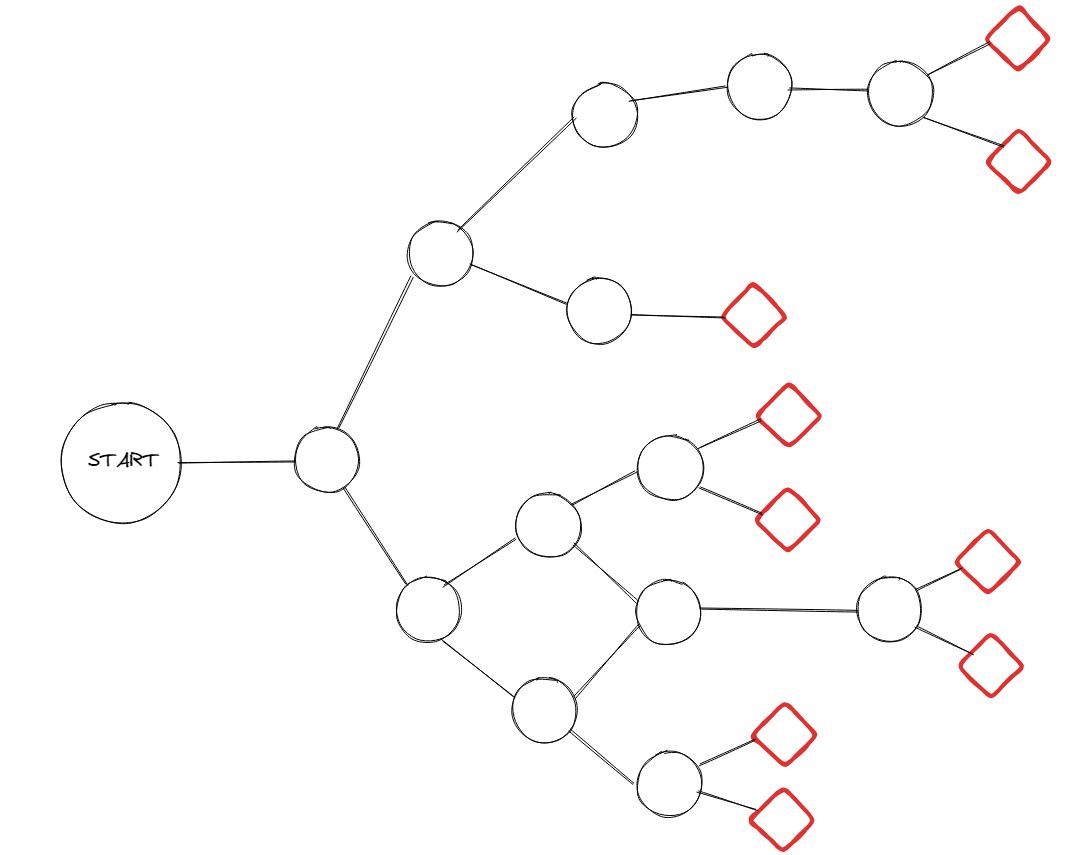
\includegraphics[width=\textwidth]{ch2_1_branching.png}
    \caption{Struktura rozgałęziająca się}
    \centering
    \label{fig:ch1_2_1_branching}
\end{figure}

\newpage

\subsection{Park rozrywki}

Struktura ta z założenia bardzo przypomina model rozgałęziający się, natomiast w tym przypadku
możemy mówić o narracji rozwijającej się ze względu na przestrzeń a nie czas\cite{theorising_narrative}.
Przykładowo, zwiedzając świat gry gracz może napotkać postać NPC, która otworzy przed nim nową
gałąź fabularną (np. poprzez zlecenia zadania do wykonania)\cite{the_evolution_of_video_games}.
Model ten jest bardzo popularny dla gier z otwartym światem, przykładem może być "Wiedźmin 3"
(Patrz \ref{subsection:ch1_2}).

\subsection{Cegiełki}

W ramach niektórych tytułów twórcy nie skupiają się na stworzeniu narracji możliwej do doświadczenia
przez grającego, lecz na pewnym systemie części, za pomocą których gracz sam jest w stanie tworzyć
historię. Części te nazywane \textit{"cegiełkami"} (ang. \textit{building blocks})\cite{theorising_narrative}
są wykorzystywane przez grającego do tworzenia własnej narracji. Przykładem tego rodzaju rozgrywki
może być tytuł "The Sims" (2000), w którym to gracz tworzy i steruje rodziną --- a co za tym idzie,
kieruje ich historią życia.

\section{Sposoby przedstawiania narracji}\label{subsection:ch1_2_2}

Oprócz zaplanowania i rozłożenia fabuły gry na części --- przy użyciu kombinacji struktur opisanych
w poprzedniej sekcji --- istotną kwestią pozostaje wybór w jaki sposób dane sekwencje fabularne
mają zostać przekazane graczowi. W ramach tej sekcji opisane zostaną najważniejsze techniki
prezentowania narracji.

\subsection{Cut scenki}\label{subsubsection:ch1_2_2_cutscene}

Jednym z najbardziej widowiskowych sposobów prezentowania treści fabularnej jest zdecydowanie
cut scenka, która zdefiniowana została przez Glassnera (2004) następująco:

\begin{quotation}
    \textit{... pre-renderowany fragment wideo ... czasami renderowany w czasie rzeczywistym przy
        użyciu sprzętu komputerowego lub konsoli. Podczas odtwarzania możliwość interakcji gracza
        zostaje zawieszona, a on sam staje się biernym widzem na czas trwania sceny}\cite{narrative_structures}
\end{quotation}

Cut scenka jest zatem po prostu fragmentem wideo. Można dokonać pewnego podziału ze względu na
sposób renderowania czy też możliwość interakcji gracza (której powyższa definicja nie przewiduje).
W ramach materiału pre-renderowanego gracz obserwuje de facto odtwarzany plik wideo, który mógł
być wyprodukowany w dowolny sposób. Typowy silnik gry nie jest w tym momencie używany, a filmik
jest prezentowany w pewnego rodzaju odtwarzaczu multimedialnym. W przypadku materiału renderowanego
w czasie rzeczywistym wykorzystywany jest silnik gry oraz modele/tekstury występujące podczas
rozgrywki. Zapewnia to zdecydowanie płynniejsze przechodzenie pomiędzy momentami nieinteraktywnymi
i interaktywnymi oraz prowadzi do większej spójności wizualnej. Wymaganie użycia sprzętu komputerowego
może prowadzić do pewnego ograniczenia jakości czy też wykorzystywanych technik (jak np. symulacji
fizycznych). Klasycznie cut scenki nie są interaktywne a gracz jest jedynie pasywnym odbiorcą.
W niektórych tytułach możemy jednak natknąć się na metodę QTE (z ang. \textit{quick time event}), w
ramach której podczas odgrywania danej scenki wyświetlają się ikonki (potencjalnie wraz z instrukcjami)
symbolizujące przycisk do wciśnięcia przez gracza. Wymusza to na nim uważność przy oglądaniu materiałów
a dodatkowo wprowadza mechanizm stresowy, ponieważ często błędnie wykonane sekwencje pociągają
za sobą konsekwencje fabularne (np. śmierć danej postaci). Cut-scenki w wersji klasycznej jak i z
uwzględnieniem QTE zostały zaprezentowane na rysunku \ref{fig:ch1_2_2_cutscene}.

\begin{figure}[h]
    \begin{subfigure}{0.49\textwidth}
        
\includegraphics[width=\linewidth, height=6cm]{ch2_2_cutscene.jpg}
        \caption{Normalna cut-scenka}
        \label{subfig:ch2_2_cutscene1}
    \end{subfigure}
    \begin{subfigure}{0.49\textwidth}
        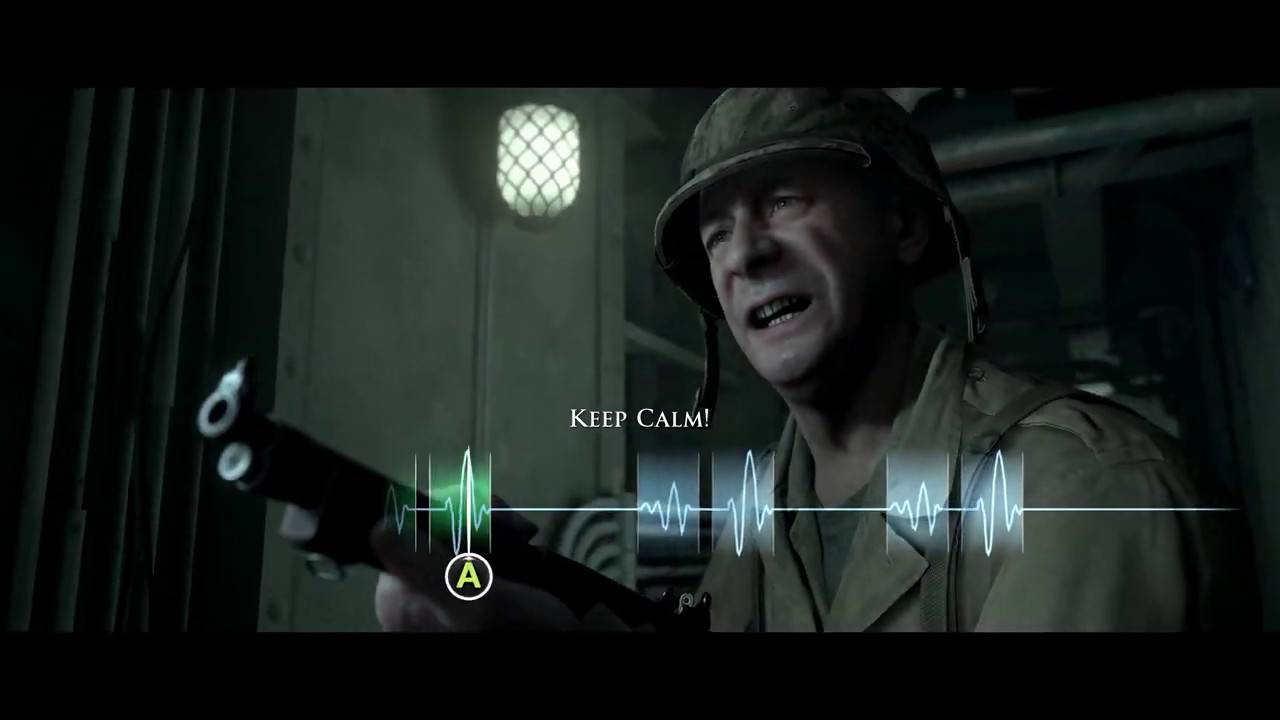
\includegraphics[width=\linewidth, height=6cm]{ch2_2_cutscene2.jpg}
        \caption{Cut-scenka z QTE}
        \label{subfig:ch2_2_cutscene2}
    \end{subfigure}
    \caption{The Dark Pictures Anthology: Man of Medan (2019) - Supermassive Games}
    \label{fig:ch1_2_2_cutscene}
\end{figure}

\newpage

\subsection{Tekst}

W przypadku tekstu możemy mówić o pełnoprawnych blokach tekstowych (Rys. \ref{fig:ch1_2_2_text}),
elementach interfejsu czy też o odpowiednich komunikatach pojawiających się na ekranie. Jest to
oczywiście bardzo prosta forma przekazu fabularnego, wzorująca się na szeroko pojętej literaturze.
Może być wykorzystany jako główny sposób prowadzenia opowieści lub jako element pomocniczny, często
robiący fabularnie sens (np. w "Final Fantasy XIII" postacie naturalnie prowadzą między sobą dialog,
ale informacje o świecie skryte w formie notatek znajdowanych przez gracza w trakie rozgrywki).

\begin{figure}[h]
    \begin{subfigure}{0.49\textwidth}
        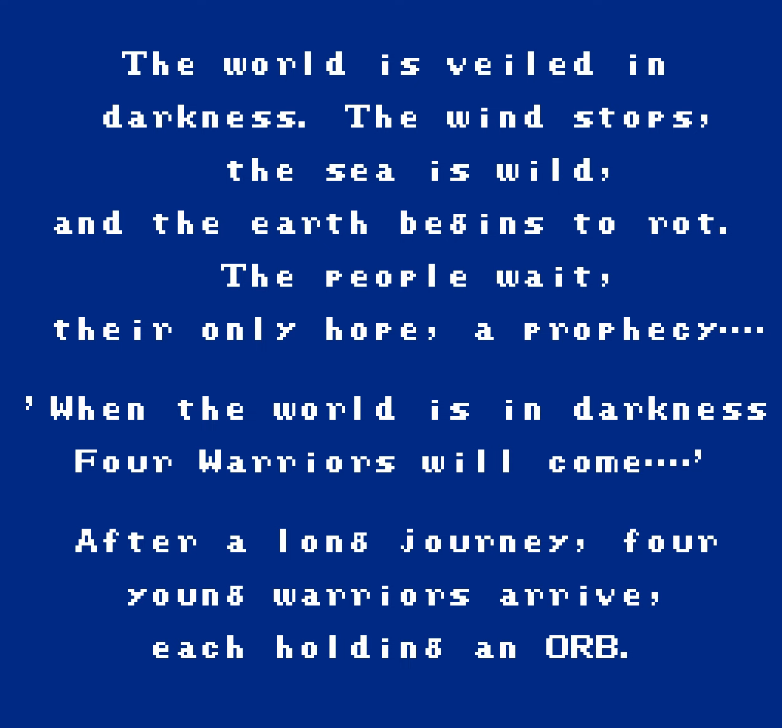
\includegraphics[width=\linewidth, height=6cm]{ch2_ff1.png}
        \caption{Final Fantasy I (1987)}
        \label{subfig:ch2_2_text1}
    \end{subfigure}
    \begin{subfigure}{0.49\textwidth}
        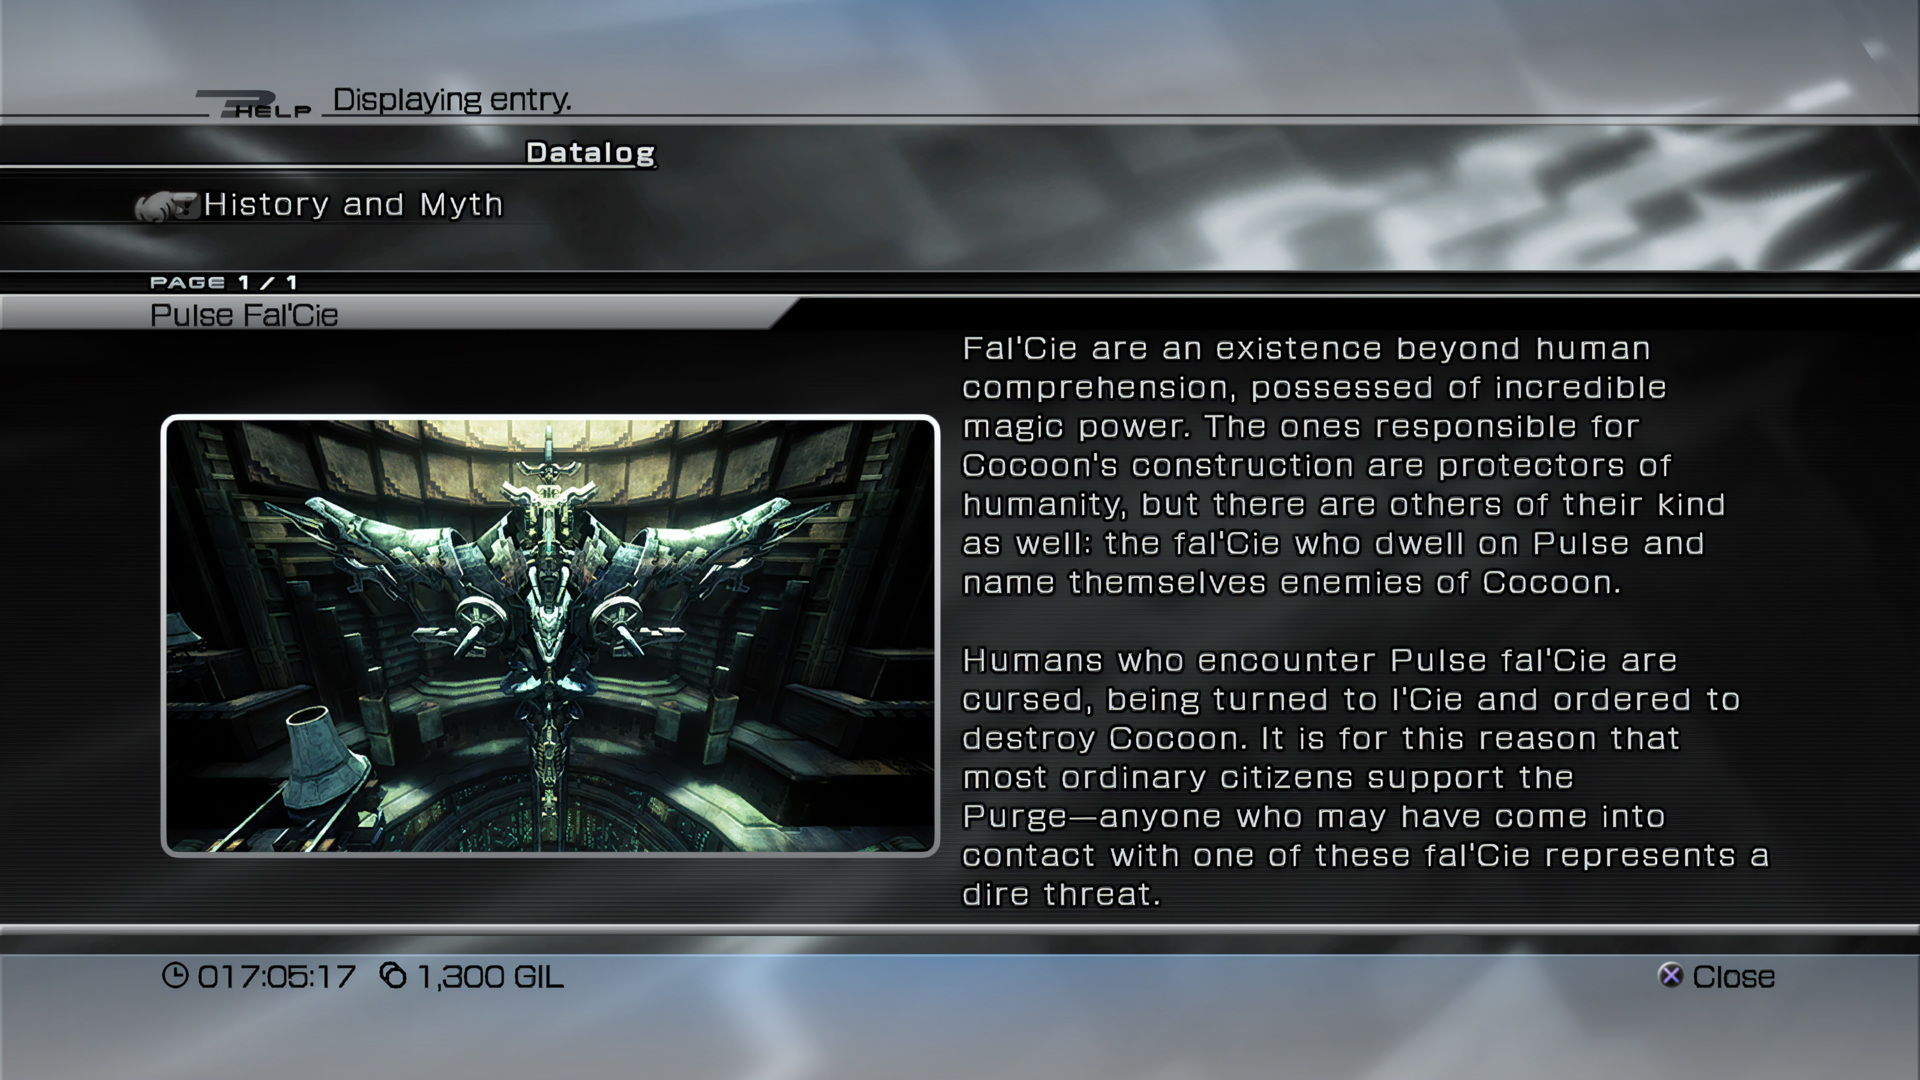
\includegraphics[width=\linewidth, height=6cm]{ch2_ff13.png}
        \caption{Final Fantasy XIII (2009)}
        \label{subfig:ch2_2_text2}
    \end{subfigure}
    \caption{Bloki tekstu służące do przedstawienia fabuły}
    \label{fig:ch1_2_2_text}
\end{figure}

\subsection{Dialogi (głównie z NPC)}

Dialog jako forma przedstawienia narracji może stanowić połączenie tekstu, dźwięku, animacji i
interaktywności. Tekst może być obecny w formie napisów pomocniczych do kwestii wypowiadanych przez
postacie, ale i również prezentuje możliwości do wyboru dostępne dla gracza. Współcześnie wiele gier
nadaje głos swoim postaciom przy pomocy aktorów głosowych. Tak jak w przypadku cut scenek w czasie
rzeczywistym, postacie najczęściej są animowane podczas dialogu, korzystając z silnika gry.
Interaktywność podczas dialogu może wyłaniać się w formie przeklikiwania kolejnych kwestii (by dać
graczowi czas na przeczytanie / zastanowienie się) lub poprzez możliwość wyboru kolejnych kwestii.
W zależności od tytułu niektóre konwersacje mogą przypominać strukturę łańcucha pereł (gdzie
rozmowa i tak kończy się w ten sam sposób) a niektóre formę rozgałęziającą się (gdzie odpowiedni
wybór może nieść za sobą dalsze konsekwencje fabularne) [Patrz \ref{subsection:ch1_2_1}]. Więcej
o systemach dialogowych wspomniane jest w sekcji \ref{subsection:ch3_1}.

\begin{figure}[h]
    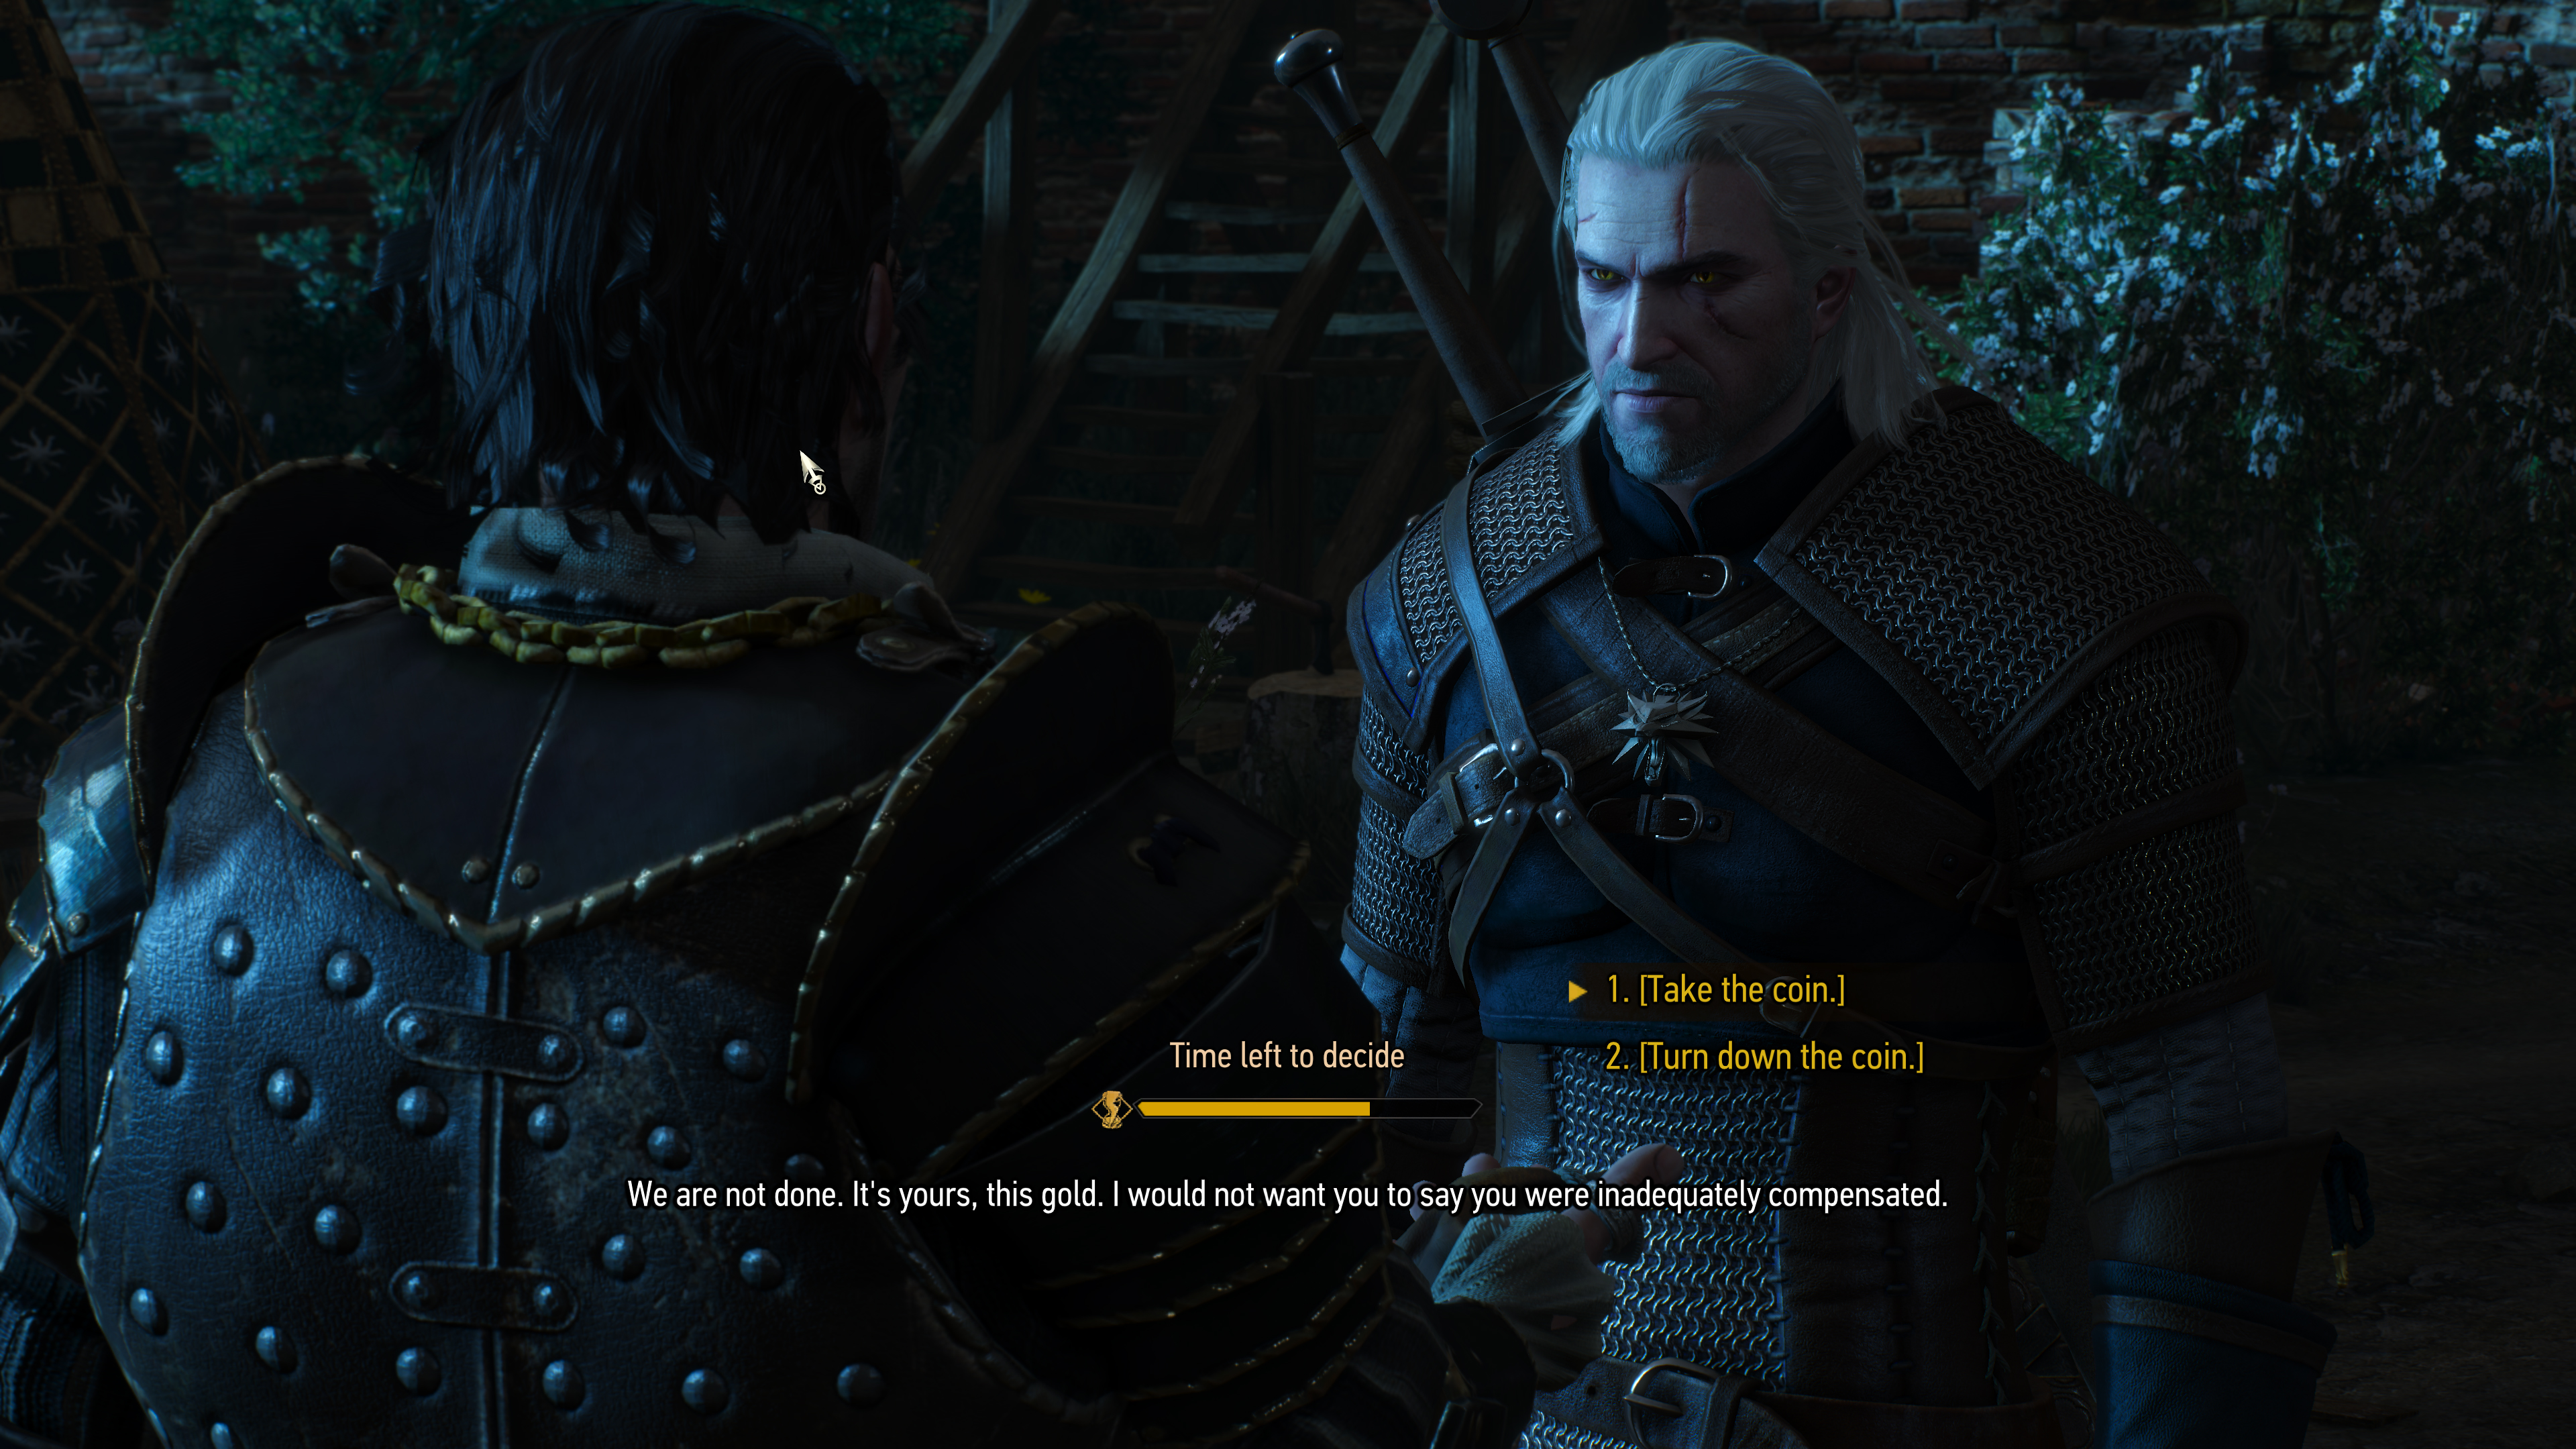
\includegraphics[width=\textwidth]{ch2_witcher_2.png}
    \caption{Dialog z NPC - "Wiedźmin 3" (2015)}
    \centering
    \label{fig:ch1_2_2_dialogue}
\end{figure}

\subsection{Poprzez świat gry (audio-wizualne)}

Najciekawszym a zarazem najrzadszym\cite{the_evolution_of_video_games} sposobem prezentowania fabuły
jest opowiadanie za pomocą samego świata gry. Mowa tu o obiektach i ich umiejscowieniu, teksturach,
ścieżkach dźwiękowych czy wszelkich innych widocznych lub słyszalnych elementach świata. Jedną z
serii gier, która bazuje na tym koncepcie i cieszy się ogromną popularnością, jest "Dark Souls".
Cut scenki są bardzo sporadyczne, przeważnie na początku i końcu rozgrywki oraz prezentujące starcie
z trudnymi przeciwnikami (\textit{"bossami"}). Spotykane postacie NPC są bardzo enigmatyczne, nie
zadają graczowi wprost zadań do wykonania i posiadają tylko kilka zapętlających się kwestii
dialogowych. Tekstowy opis dotyczy głównie znajdowanych przedmiotów i zawiera szczątkowe informacje
dotyczące ogólnopojętego świata gry. W ten sposób gracz musi samemu układać fabułę, na podstawie
znajdowanych skrawków wiedzy. Dodatkowo, muzyka występuje tylko w ramach pojedynczych lokacji albo
w przypadku starć z \textit{"bossami"}. W ten sposób autorzy podkreślają wagę tego co jest właśnie
prezentowane na ekranie i starają się wywołać u gracza pewne emocje.
\graphicspath{{chapters/chapter3/imgs/}}

\chapter{Zaangażowanie gracza}\label{chapter:ch3}

By móc określić wpływ rozwiązań sztucznej inteligencji na angażującą narrację wewnątrz gry należy
zdefiniować w jaki sposób określić i mierzyć można zaangażowanie gracza. W tej sekcji podjęta
zostanie próba skategoryzowania zaangażowania i wybrania najodpowiedniejszej metody do wykorzystania
w ramach eksperymentu.

\section{Definicje i rodzaje zaangażowania}\label{section:ch3_1}

Pomiar i ocena zaangażowania graczy w gry wideo jest niezwykle skomplikowanym zadaniem.
Podstawową przeszkodą jest to, że zaangażowanie nie jest zjawiskiem jednowymiarowym\cite{eng_in_games}, łatwym do
uchwycenia\cite{measuring_user_exp}. Stanowi raczej złożony, subiektywny stan umysłu, na który składać się
może wiele elementów. W literaturze naukowej poświęconej temu zagadnieniu można najczęściej spotkać się z terminami
takimi jak: imersja, obecność, przepływ / trans, absorpcja psychologiczna czy dysocjacja. Podstawowym problemem
jest fakt, że doświadczenia przeżywane podczas rozgrywki różnią się ze względu na gatunek gry, na stan
emocjonalny / psychiczny grającego czy też ze wględu na jego charakter\cite{measuring_user_exp}.

Kolejnym kluczowym utrudnieniem jest fakt, iż zaangażowanie oparte jest na
nieświadomych procesach poznawczych i emocjonalnych, do których trudno uzyskać
introspekcyjny dostęp\cite{measuring_user_exp}. Wymaganie od gracza, by w trakcie rozgrywki analizował i werbalizował swoje
przeżycia, nieuchronnie zakłóca i niszczy stan umysłu będący celem badań.
Zaangażowanie jest więc zjawiskiem dość ulotnym, które może w pełni przeminąć po wyciągnięciu grającego
ze sfery skupienia\cite{measuring_user_exp}.

Problemy pojawiają się również przy próbach retrospektywnego opisu i oceny zaangażowania po zakończeniu
sesji gry. Brakuje w tym obszarze nauki pewnego wspólnego słownika, dzięki któremu uczestnicy badań mogliby
w sposób jednoznaczny zwerbalizować subtelności tego złożonego doświadczenia\cite{measuring_user_exp}.
Ograniczeni jesteśmy do używania bardzo ogólnych terminów takich jak "frajda",
"zaangażowanie" czy "zaabsorbowanie", które nie oddają do końca bogactwa i głębi przeżywanych
stanów\cite{measuring_user_exp}.

Co więcej, zaangażowanie jest zjawiskiem silnie zależnym od otaczającego ją kontekstu, na który
składać się może sama rozgrywka ale i również interakcje społeczne czy fizyczne środowisko, w
którym znajduje się grający. Wszelkie próby jej wyizolowania i uproszczenia do czysto indywidualnego
doświadczenia gruntownie zniekształcają jego naturę.

W badaniach nad zaangażowaniem istotne są prace, które pomogły zdefiniować, gdzie ono rezyduje w
odniesieniu do szerokiego spektrum wymiarów lub stanów poznawczych i emocjonalnych, takich jak motywacja
i poczucie własnej skuteczności. Teoria samookreślenia pomaga wyjaśnić między innymi w jaki
sposób motywacja wewnętrzna - napędzana czynnikami takimi jak potrzeba kompetencji - jest ważnym
prekursorem zaangażowania. Zaangażowanie jest jednak czymś zgoła odmiennym od motywacji\cite{measuring_engagement}.
Można je postrzegać jako serię czasowych interakcji podczas wykonywania zadania, podczas gdy motywacja to
bardziej uniwersalne osobiste nastawienie wobec nauki/zadania. Połączenie tych dwóch stanów, czyli
zaangażowanie osoby w zadanie, do którego jest ona zmotywowana, może skutkować poczuciem satysfakcji
i chęci ponownego zaangażowania się w to zadanie\cite{measuring_engagement}.

Przedstawione zostaną najczęściej występujące w literaturze terminy pokrewne lub stanowiące część
zaangażowania:

\begin{itemize}
      \item Imersja (ang. \textit{Immersion})
      \item Obecność (ang. \textit{Presence})
      \item Przepływ / trans  (ang. \textit{Flow})
      \item Absorpcja (ang. \textit{Absorption})
      \item Dysocjacja (ang. \textit{Dissociation})
\end{itemize}

\begin{description}
      \item[Imersja] (zanurzenie) w grach wideo jest szeroko dyskutowanym pojęciem w pracach
            naukowych. Imersja zazwyczaj opisuje doświadczenie zaangażowania się w grę, przy zachowaniu pewnej
            świadomości otoczenia, a definiuje się ją także jako zdolność gry do wywoływania uczucia bycia
            częścią, czy "obecności" w wirtualnym środowisku gry. Przewiduje się, że niemal każdy przeciętny grający
            doświadcza pewnego stopnia imersji\cite{development_of_game}. Imersja (również nazywana "imersją
            sensoryczną i wyobrażeniową") oznaczać może również jak silne połączenie z grą odczuwał gracz\cite{validation_of_ge_scales}.
            Istnieją dyskusje na temat prawidłowej specyfikacji konstruktu imersji - czy powinien być modelowany
            jako refleksyjno-refleksyjny, czy refleksyjno-formatywny\cite{eng_in_games}.
      \item[Obecność] w kontekście gier wideo i wirtualnej rzeczywistości jest pojęciem, które
            wciąż ewoluuje i oczekuje na ostateczną definicję, jednak zazwyczaj jest określana jako połączenie
            tych dwóch aspektów: 1. Bycie w normalnym stanie świadomości oraz 2. Doświadczanie poczucia znajdowania się
            wewnątrz wirtualnego środowiska\cite{development_of_game}. Większość, ale nie wszyscy gracze, prawdopodobnie mają zdolność do
            doświadczania obecności w odpowiednich warunkach\cite{development_of_game}. Poczucie obecności w
            alternatywnym środowisku może wynikać ze stymulacji sensorycznej\cite{measuring_narrative}.
            Ogólniej, obecność wiąże się z emocjonalnym zaangażowaniem w grę\cite{validation_of_ge_scales}.
      \item[Przepływ / trans] najczęściej występuje w literaturze anglojęzycznej pod pojęciem \textit{flow}.
            Przepływ można postrzegać jako głębokie, imersyjne doświadczenie, które wynika z zaangażowania się
            osoby w zadanie o odpowiedniej równowadze pomiędzy wyzwaniem a poziomem umiejętności użytkownika\cite{measuring_engagement}.
            Przepływ i rozgrywka w grach są często łączone w kontekstach, gdzie użytkownik napotyka znaną (przykładowo
            z innych tytułów) strukturę rozgrywki natomiast doświadcza nowej treści (fabularnej,
            audio-wizualnej itd.)\cite{measuring_engagement}. Przepływ to termin opisujący uczucie przyjemności, które występuje, gdy osiąga
            się równowagę pomiędzy umiejętnościami a wyzwaniem w procesie wykonywania wewnętrznie nagradzającej
            aktywności\cite{development_of_game}. Posiadanie określonego celu i natychmiastowej informacji zwrotnej o wynikach zwiększa
            prawdopodobieństwo wystąpienia przepływu, a bycie w stanie przepływu wydaje się mieć wpływ na przebieg nauki
            użytkownika. Stany przepływu obejmują również uczucie kontroli, bycia jednością z aktywnością i doświadczanie
            zniekształceń czasu. Ponieważ wiąże się z doświadczaniem zmienionego stanu świadomości, doświadczenie
            przepływu może być nieco mniej powszechne niż imersja czy obecność\cite{development_of_game}. Z perspektywy modeli mentalnych
            przepływ do narracji występuje wtedy, gdy odbiorca całkowicie skupia się na czynności zrozumienia -
            tworzenia i aktualizowania modeli mentalnych reprezentujących historię\cite{measuring_narrative}.
      \item[Absorpcja] to termin używany do opisania całkowitego zaangażowania w bieżące doświadczenie. W
            przeciwieństwie do imersji i obecności, a podobnie do przepływu, stan absorpcji psychologicznej
            wiąże się ze zmienionym stanem świadomości\cite{development_of_game}. Ogólną skłonność osoby do wchodzenia
            w stan absorpcji psychologicznej można określać jako cechę, podczas gdy doświadczenie
            wchodzenia w ten stan w określonej aktywności najlepiej postrzegać jako stan przejściowy\cite{development_of_game}.
            Niektóre badania dotyczące modeli zaangażowania w grę twierdzą, że absorpcja jest zasadniczo formą
            przepływu. Wtedy też lepiej wykluczyć ją z ostatecznego modelu zaangażowania w grę\cite{eng_in_games}.
      \item[Dysocjacja] znana jest jako objaw kliniczny występujący u osób cierpiących na traumę, natomiast
            naturalnie występuję również jej niepatologiczna forma\cite{development_of_game}.
            Najbardziej powszechnym przykładem dysocjacji niepatologicznej u dorosłych jest "hipnoza drogowa".
            Kierowcy wchodą wtedy w stan absorpcji z aktywnością niezwiązaną z prowadzeniem.
            Równocześnie, konieczne obowiązki związane z manewrowaniem
            pojazdem są dalej wykonywane, pomimo że procesy mentalne związane z prowadzeniem są oddzielone
            od świadomej myśli\cite{development_of_game}.
\end{description}

\section{Sposoby pomiaru zaangażowania gracza}\label{section:ch3_2}

Istnieje wiele różnych podejść do pomiaru zaangażowania gracza, które cechują się odpowiednimi wadami i zaletami.
Metody fizjologiczne, takie jak monitorowanie tętna, częstości oddychania, aktywności
mięśniowej (elektromiografia), fal mózgowych (elektroencefalografia) oraz przewodnictwo skórne,
zapewniają większą obiektywność danych, ale są zwykle droższe (pod względem czasowym i finansowym) oraz
trudniejsze w interpretacji\cite{validation_of_ge_scales}.
Analiza zachowań graczy w grze (telemetria) również oferuje obiektywność,
natomiast wciąż pewnego rodzaju wyzwanie stanowi redukcja złożoności związanej z
profilowaniem oraz powiązanie zachowań w grze z subiektywnym doświadczeniem gracza. Z drugiej strony,
bardziej subiektywne metody oceny zaangażowania gracza, takie jak wywiady, grupy fokusowe, sondy w grze oraz
kwestionariusze, są stosunkowo tańszymi alternatywami i charakteryzują się mniejszymi trudnościami w
interpretacji niż pomiary fizjologiczne czy telemetria\cite{validation_of_ge_scales}.
Wywiady, grupy fokusowe i sondy w grze pozwalają dogłębniej poznać odczucia grających, ale trudno je przeprowadzić na
dużą skalę. W przeciwieństwie do nich, kwestionariusze można łatwo dystrybuować wśród bardzo dużych grup,
i mimo że dostarczają mniej dogłębnych informacji niż inne subiektywne metody, umożliwiają skoncentrowanie
się na konkretnych aspektach zaangażowania gracza\cite{validation_of_ge_scales}.

W celu zewaluowania zaangażowania graczy w eksperymencie przeprowadzonym w ramach tejże pracy
zdecydowano się na pomiar w formie kwestionariusza.
Wybór konkretnego narzędzia ułatwiła praca Normana\cite{geq}, który porównał ze sobą dwa modele kwestionariusza
zaangażowania w grę (Game Engagement/Experience Questionnaire - GEQ)\cite{development_of_game}\cite{game_exp_quest}. Ostatecznie wybrano model
zaproponowany przez Brockmyera i współpracowników\cite{development_of_game}, który charakteryzuje się kilkoma istotnymi cechami.
Po pierwsze, podejście Brockmyera i in.\cite{development_of_game} koncentruje się na ocenie skłonności pojedynczego grającego do
zaangażowania się w grę wideo, a nie na ocenie samej gry\cite{geq}. Autorzy\cite{development_of_game} zaczęli od
zaledwie 10 pozycji z pięciostopniową skalą ocen. Dodatkowe pozycje zostały stworzone, aby lepiej
odzwierciedlić zaangażowanie, a cały kwestionariusz został następnie poddany ocenie na dwóch różnych próbach: 213 uczniów szkoły
średniej i 51 studentów. Analizy wykazały potrzebę dodania kolejnych pozycji, doprowadzając do powstania
19-punktowego kwestionariusza. Mimo że nie wyjaśniono, skąd pochodziły nowe pozycje, kwestionariusz ten
wykazuje dobre statystyki niezawodności\cite{geq}, z współczynnikiem alfa Cronbacha na poziomie 0,85 oraz estymacją
niezawodności osoby na poziomie 0,83 i niezawodności pozycji na poziomie 0,96 w modelu Rascha\cite{development_of_game}.
Ponadto, Brockmyer i współpracownicy\cite{development_of_game}
skupili się na jednowymiarowym kontinuum określanym jako "zaangażowanie", co jest główną zaletą ich
pracy\cite{geq}. Autorzy przyznają jednak, że rekrutowali często grające osoby płci męskiej,
aby zwiększyć prawdopodobieństwo doświadczenia głębokiego zaangażowania w grę w sytuacji
laboratoryjnej, co sugerować może potrzebę ponownej ewaluacji kwestionariusza na szerszej próbie\cite{geq}.

W ramach eksperymentu z kwestionariusza GEQ zaproponowanego przez Brockmyera i in.\cite{development_of_game}, cztery
pozycje zostały zastąpione odpowiednikami pochodzącymi z modelu IJsselsteijn'a\cite{game_exp_quest}. Decyzja ta podyktowana
była faktem, iż konkretne pozycje z kwestionariusza IJsselsteijn'a\cite{game_exp_quest} lepiej odzwierciedlają nastawienie gracza wobec
narracji przedstawianej w grze podczas pojedynczej sesji rozgrywki. Ponieważ eksperyment koncentruje się na ocenie
zaangażowania w trakcie krótkich pojedynczych sesji, zastąpienie wybranych pozycji umożliwiło lepsze
dopasowanie narzędzia do specyficznych warunków badania.

\begin{table}[ht]
      \begin{center}
            \begin{tabular}{|r | l|}
                  \hline
                  Number      & Question                                       \\
                  \hline
                  1           & I lose track of time                           \\
                  \textbf{2}  & \textbf{I was interested in the game's story}  \\
                  3           & I feel different                               \\
                  4           & I felt that I could explore things             \\
                  5           & The game feels real                            \\
                  \textbf{6}  & \textbf{I was fully occupied with the game}    \\
                  7           & I get wound up                                 \\
                  8           & Time seems to kind of stand still or stop      \\
                  9           & I feel spaced out                              \\
                  \textbf{10} & \textbf{I was deeply concentrated in the game} \\
                  11          & I got tired\footnotemark{}                     \\
                  12          & Playing seems automatic                        \\
                  13          & My thoughts go fast                            \\
                  \textbf{14} & \textbf{I enjoyed it}                          \\
                  15          & I play without thinking how to play            \\
                  16          & Playing makes me feel calm                     \\
                  17          & I play longer than I meant to                  \\
                  18          & I really get into the game                     \\
                  19          & I feel like I just can't stop playing          \\
                  \hline
            \end{tabular}
      \end{center}
      \caption{Zmodyfikowany kwestionariusz GEQ}\label{tab1:ch3_2}
\end{table}

\newpage

W tabeli \ref{tab1:ch3_2} przedstawiono zmodyfikowany kwestionariusz Brockmyer'a\cite{development_of_game}
o cztery pozycje pochodzące bezpośredniu z modelu IJsselsteijn'a\cite{game_exp_quest}
(zaznaczone zostały poprzez pogrubienie). \footnotetext{Oryginalnie w formie "I can't tell that I'm getting tired" co mogło być mylące w przypadku odpowiedzi tak/nie}
\graphicspath{{chapters/chapter4/imgs/}}

\chapter{Sposoby generowania narracji}\label{chapter:ch4}

W poprzednich sekcjach omówiona została historia gier oraz wykorzystywane w grach komputerowych rodzaje
narracji. W każdym z tych elementów istnieje jedna część wspólna: to ludzie odpowiadają za tworzenie
historii, odpowiednie jej planowanie i prezentowanie odbiorcy. Związane z tym są oczywiście olbrzymie
koszty oraz duży nakład czasu poświęcony przez pracowników. Biorąc pod uwagę terminy stale goniące
producentów gier, nic dziwnego, że pewne zaplanowane fragmenty fabularne nie znajdują miejsca w~końcowym
produkcie. Z tego względu, patrząc na postępujący rozwój technologiczny, nasuwa się pytanie ---
czy da się zarządzać narracją w grze komputerowej w sposób automatyczny? W ramach tej sekcji
przedstawione zostaną znane rozwiązania z dziedziny sztucznej inteligencji pomagające w kreowaniu fabuły
oraz nakreślony zostanie potencjał w tej sferze dużych modeli językowych.

\section{Wykorzystanie algorytmów sztucznej inteligencji do kreowania narracji}\label{section:ch4_1}

Mówiąc o ogólnym wykorzystaniu algorytmów sztucznej inteligencji można cofnąć się do bardzo prostych
rozwiązań wykorzystanych np. w "Pong" (Patrz sekcja \ref{subsection:ch1_2}), do technik generowania
proceduralnego (zwłaszcza poziomów) czy też do systemów rankingowych (np. system TrueSkill). Jako, że
nie są to metody stricte powiązane z narracją to nie zostaną one opisane bardziej szczegółowo.
Przedstawione natomiast będą kluczowe obszary wykorzystywane w grach: częściowo-uporządkowane planowanie
(ang. \textit{\gls{pop}} - partially-ordered planning), modelowanie doświadczeń gracza (ang. \textit{\gls{pem}} -
player experience modelling), przetwarzanie języka naturalnego (ang. \textit{\gls{nlp}} - natural language
processing), postać niegrywalna (ang. \textit{\gls{npc}} - non-playable character), proces decyzyjny Markowa
(ang. \textit{\gls{mdp}} - Markov decision process).

\subsubsection*{POP (Partially-ordered planning)}

Planowanie częściowo-uporządkowane jest skierowanym grafym acyklicznym, gdzie węzły są operacjami
(inaczej nazywanymi akcjami), które po wywołaniu zmieniają stan świata. Krawędzie przedstawiają
relacje przyczynowe i czasowe pomiędzy akcjami. Powiązanie przyczynowe $a_{i} \rightarrow^{c}a_{j}$
oznacza, że wykonanie akcji $a_{i}$ zmieni stan warunku $c$ na prawdziwy w świecie fabuły, a co za
tym idzie akcja $a_{j}$ zależna od tego warunku będzie możliwa do wykonania. Powiązanie czasowe
przedstawia ograniczenie porządkowe pomiędzy operacjami, gdzie jedna operacja musi być wykonana przed
inną\cite{game_ai_storytelling}. Przykładowa struktura fabularna zrealizowana za pomocą planowania
częściowo-uporządkowanego została przedstawiona na rysunku \ref{fig:ch4_1_pop}.

\begin{figure}[h]
    \centering
    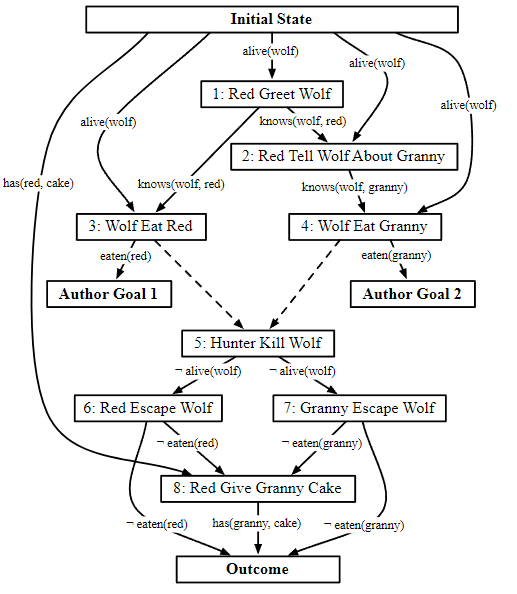
\includegraphics[width=0.5\textwidth]{ch4_1_pop.png}
    \caption{Fabuła "Czerwonego Kapturka" zapisana za pomocą POP}
    \label{fig:ch4_1_pop}
\end{figure}

Za pomocą tej techniki kreować można rozbudowane plany fabularne, które mogą ulegać zmianie na
podstawie akcji podejmowanych przez gracza czy zmian zachodzących w~świecie gry. Odpowiednie algorytmy
przeszukiwania nazywane \textit{"plannerami"} rozwiązują problem planowania, tzn. mając dany stan
świata, pewne atomowe akcje możliwe do wykonania przez grającego oraz założony cel, znajdują
odpowiednią sekwencję operacji, które doprowadzą do osięgnięcia tegoż celu\cite{game_ai_storytelling}.

Podstawowym problemem pojawiającym się przy wykorzystaniu metody \gls{pop} jest to, że zarówno gracz jak i
potencjalnie inne niegrywalne postacie, mogą być zdolne do wywołania akcji w świecie gry, która
zagraża dalszemu przebiegowi fabularnemu zgodnego z planem\cite{characters_and_directors}. Wtedy
stosowane są odpowiednie techniki naprawcze, które prowadzą do mniej lub bardziej doskonałych rozwiązań.

\subsubsection*{PEM (Player experience modelling)}

Modelowanie doświadczeń gracza polega na zbieraniu danych behawioralnych czy też wydajnościowych
(punkty, czas, decyzje) ze względu na rozgrywkę za pomocą wielu modalności: mowy gracza, obrazów
(śledzenie ruchów ciała, mimiki twarzy, gałek ocznych) czy też sygnałów fizjologicznych (puls czy
przewodność skóry). Pomiar sygnałów fizjologicznych jest oczywiście problematyczny ze względu na
wykorzystanie dodatkowego sprzętu a zarazem inwazyjność przeszkadzającą w swobodnej rozgrywce
\cite{reusable_game_ai}.

W ramach tego obszaru sztuczna inteligencja objawia się zazwyczaj pod postacią sieci neuronowych czy
też drzew decyzyjnych, które pozwalają dokonywać klasyfikacji w~zakresie\cite{reusable_game_ai}:

\begin{itemize}
    \item rozpoznawania emocji grającego - w ramach anagażujących systemów dialogowych
    \item balansowania rozgrywki - tak by gracz nie odczuwał frustracji ze względu na zbyt wysoki poziom
          trudności a zarazem by nie doznawał nudy ze względu na zbyt prostą rozgrywkę
    \item oceniania umiejętności gracza - do prowadzenia badań w sposób ukryty
\end{itemize}

\subsubsection*{NLP (Natural language processing)}

Przetwarzanie języka naturalnego jest dziedziną w obrębie sztucznej inteligencji, która zajmuje się
zrozumieniem, interpretacją i manipulacją ludzkiego języka\cite{reusable_game_ai}. W ramach gier
komputerowych pozwala to graczowi poruszać się po świecie czy też komunikować z~innymi postaciami \gls{npc}
w sposób zarówno naturalny (zamiast wchodzenia w interakcję z odpowiednimi interfejsami) jak i dość
otwarty (na tyle na ile dany system jest w stanie przetwarzać odpowiednie frazy).

Z podstaw przetwarzania języka naturalnego korzystały tytuły realizowane w konwencji interaktywnej
fikcji, takie jak "Otchłań" (Patrz sekcja \ref{subsection:ch3_2}). Pozwalają one graczowi za pomocą
określonego zestawu komend poruszać się i wchodzić w interakcję z całym światem gry.

Związane z tą dziedziną są duże modele językowe, które potrafią operować językiem naturalnym.
Ich bardziej szczegółowy opis będzie przedstawiony w sekcji \ref{section:ch4_2}.

\subsubsection*{NPC (Non-playable character)}

Postacie niegrywalne to wszelkie jednostki czy postacie, z którymi gracz może wchodzić w
interakcję lub dostrzegać ich autonomiczne poruszanie w świecie. Mogą to być statyczne byty,
które usytuowane są w jednym określonym miejscu i mają na celu dawać grającemu zadania czy też
informacje o świecie gry. Z drugiej strony wszelkie jednostki, z~którymi gracz walczy również
podlegają pod tę definicję. Forma postaci niegrywalnych, tak jak i w literaturze, nie jest
istotna, gdyż bohaterem może być zarówno człowiek jak i~zantropomorfizowane zwierzę czy rzecz.

\gls{npc} pojawiły się w grach z początkiem lat 90-tych. Oparte były przede wszystkim na zpredefiniowanych
skryptach i drzewach decyzyjnych\cite{storytelling_through} (współcześnie nadal wiele postaci jest
opartych o te rozwiązania)\cite{from_pong_to_narrative}.

Wraz z rozwojem technologicznym twórcy gry mają możliwość przeznaczenia więcej mocy obliczeniowej
na wiarygodne dla gracza postacie \gls{npc}. Związane jest to z dokładniejszymi modelami i animacjami
postaci ale również z bardziej zaawansowanymi wzorcami zachowania. Producenci zaczęli wykorzystywać
od lat 2010 w tym celu techniki uczenia maszynowego oraz głębokiego nauczania
\cite{from_pong_to_narrative}. Pozwala to przeciwnikom (czy też sprzymierzeńcom) gracza
dostosowywać się do sposobu prowadzenia przez niego rozgrywki. Współczesne tytuły takie jak
"Read Dead Redemption 2" czy "The Last of Us Part II" wykorzystują głębokie sieci neuronowe do
budowania postaci \gls{npc}\cite{from_pong_to_narrative}.

\subsubsection*{MDP (Markov decision process)}

Łańcuch Markowa jest stochastycznym modelem opisującym ciąg możliwych zdarzeń, w którym
prawdopodobieństwo każdego zdarzenia zależy jedynie od wyniku poprzedniego. Rozróżniane one
są dodatkowo ze względu na dyskretne lub ciągłe momenty czasowe, w których następuje zmiana
stanów. Proces decyzyjny Markowa (\gls{mdp}) jest zasadniczo rozszerzeniem łańcuchów Markowa ---
różnicę stanowi dodanie akcji (które pozwalają na podejmowanie decyzji) oraz nagród otrzymywanych
po przejściu z jednego stan w drugi. Jeżeli dla każdego stanu istnieje tylko jedna akcja i
wszystkie nagrody są jednakowe, to proces decyzyjny Markowa upraszcza się do łańcucha Markowa.

\begin{figure}[h]
    \centering
    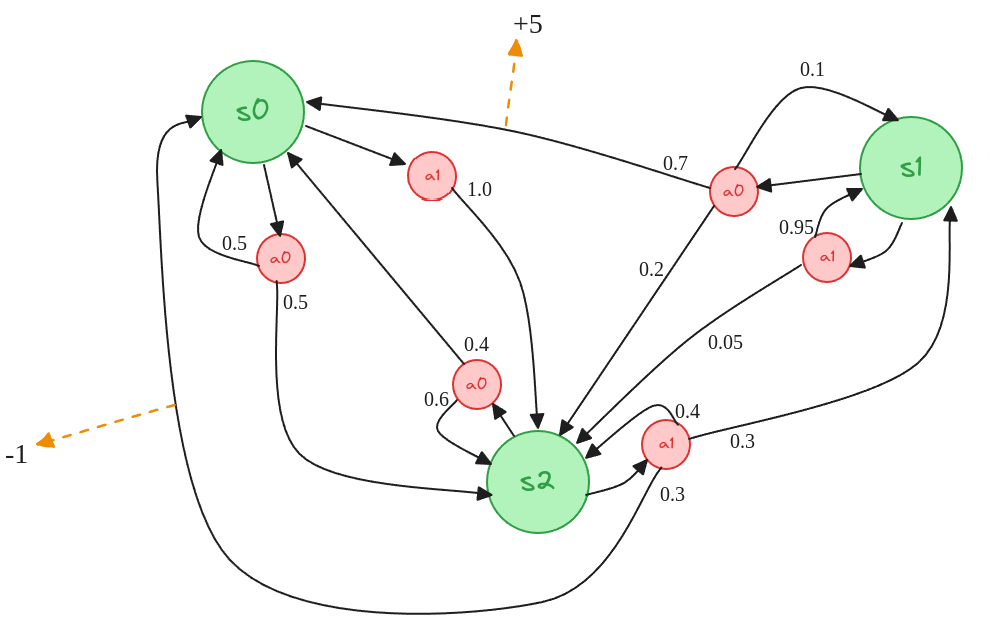
\includegraphics[width=0.8\textwidth]{ch4_1_mdp.png}
    \caption{Przykładowy proces decyzyjny Markowa}
    \label{fig:ch4_1_mdp}
\end{figure}

Na powyższym rysunku przedstawiony został przykładowy proces decyzjny Markowa z~trzema stanami (zielone
kółka), dwiema akcjami (czerwone kółka) oraz dwiema nagrodami (pomarańczowe strzałki). Model \gls{mdp} może
być wykorzystany w ramach generowania treści gier komputerowych do budowania zadań dla gracza,
przykładowo dla gry kucharskiej baza składników może być ułożona w odpowiednie łańcuchy Markowa, tak
by bardziej pasujące do siebie składniki miały większe prawdopodobieństwo bycia wspólnie wybranym
\cite{ammanabrolu2020automated}.

Proces może być dodatkowo wykorzystany w proceduralnym generowaniu treści czy świata dla gracza.
Zakładając, że to gracz jest \textit{"agentem"} podejmującym akcje w świecie gry (które są jawnie
zdefiniowane przez twórców), doprowadza on do zmiany stanu świata co jest idealnie reprezentowane
przez proces decyzyjny Markowa\cite{automated_planning}.

\subsubsection*{Przykład wykorzystania - "Façade"}

"Façade" (2005) to tytuł, który próbował złamać znany do tamtej pory podział na narrację liniową czy też
rozgałęziającą się, na rzecz w pełni interaktywnej historii kontrolowanej przez gracza. Jest to
trójwymiarowa gra czasu rzeczywistego przedstawiona w formie jednego aktu. Narracja koncentruje się
wokół Grace i Tripa, małżeństwa po trzydziestce, które zaprasza gracza na drinka. Gracz nie wie, że ich
małżeństwo znajduje się na grząskim gruncie, a tego wieczoru wszystkie ich małżeńskie problemy wyjdą na
jaw. To, w jaki sposób ich związek się rozpadnie, a także ostateczny związek gracza z Grace i Tripem,
zależy od interakcji gracza ze światem. Gracz angażuje się poprzez poruszanie się po środowisku,
manipulowanie przedmiotami i, co najważniejsze, poprzez dialogi w języku naturalnym\cite{1024751}.

Twórcy na potrzebę "Façade" stworzyli własny język ABL (\textit{"A Behavior Language"} - z~ang. język
zachowań). Stanowi on pewnego rodzaju połączenie drzew decyzjnych i~procesów decyzjnych Markowa
wspomnianych wcześniej. Programy ABL są zorganizowane jako zbiór zachowań, które mogą być przetwarzane
sekwencyjnie lub równolegle. Dodatkowo, zachowania mogą mieć narzucone określone wymagania by
mogły one się odbyć, a w~zależności od powodzenia lub porażki w realizacji zachowania świat gry
może zostać odpowiednio zmieniony.

\section{Wykorzystanie dużych modeli językowych (LLM) do kreowania narracji}\label{section:ch4_2}

W ostatnich latach coraz większa liczba prac naukowych oraz rozwiązań komercyjnych skupia się wokół
tzw. dużych modeli językowych. Okazuje się bowiem, że wprowadzając optymalizacje w sferze oprogramowania
czy też po prostu przeznaczając więcej mocy obliczeniowej na wyuczenie takowych modeli, zyskuje się
adekwatnie większą \textit{"skuteczność"} jeżeli chodzi o wykonywane przez nie zadania z zakresu
przetwarzania języka naturalnego (i nie tylko!).

W związku z tym nasuwa się następujące pytanie --- czy można wykorzystać \textbf{aktualne} duże modele
językowe do skutecznego kreowania narracji? W ramach tej sekcji przedstawiona zostanie dokładniejsza
charakterystyka tych modeli a zarazem istniejące próby ich wykorzystania.

\subsubsection*{Definicja i charakterystyka dużych modeli językowych}

Duże modele językowe są modelami nauczania maszynowego, które są w stanie wykonywać zadania z dziedziny
przetwarzania języka naturalnego, takie jak generowanie tekstu, tłumaczenie tekstu z jednego języka
na inny czy prowadzenie rozmowy z człowiekiem w sposób konwersacyjny\cite{larp_language}. Pojęcie
"duże" oznacza w tym przypadku zarówno skalę samych modeli (miliardy czy biliony parametrów) jak i
wymaganą do ich wyuczenia ilość danych. Pojęcie \gls{llm} skoncentrowane jest zasadniczo wokół funkcjonalności
danego modelu, niezależnie od przyjętej do jego wyuczenia architektury.

Z uwagi na fakt, że zdecydowana większość modeli oparta jest na architekturze transformera to zostanie
ona krótko nakreślona. Dane podawane na wejście do modelu mogą być różnych modalności np. tekst,
audio czy obraz. Następnie, dane te dzielone są na tzw. żetony (ang. \textit{tokens}) - fragmenty tekstu,
obrazu lub dźwięku. Każdy żeton jest kodowany jako wielowymiarowy wektor liczbowy, odzwierciedlający
jego semantyczne właściwości. Następnie sekwencja wektorów przechodzi przez blok uwagi (ang.
\textit{attention}), gdzie wektory wzajemnie się aktualizują (ponieważ np. znaczenie słowa zależy od
kontekstu, czyli od słów występujących dookoła niego). Ten proces pozwala na lepsze zrozumienie
zależności pomiędzy elementami wejściowymi. Po bloku uwagi, wektory są przetwarzane przez
perceptron wielowarstwowy (ang. \textit{MLP - multi-layer perceptron}). Cykl bloków uwagi i~MLP jest
wielokrotnie powtarzany. Na końcu procesu otrzymywana jest pojedyncza macierz, na podstawie której, poprzez
operację softmax, generowany jest rozkład prawdopodobieństwa dla możliwych żetonów następujących po
danym fragmencie wejściowym. Autorzy raportu technicznego dotyczącego \gls{gpt}-4 zauważają, że:

\begin{quote}
    \textit{"...Takie modele są ważnym obszarem badań, ponieważ mają potencjał do wykorzystania w szerokim
        zakresie zastosowań, takich jak systemy dialogowe"}\cite{openai2024gpt4}
\end{quote}

Można również wnioskować, że następne iteracje modeli będą coraz lepsze:

\begin{quote}
    \textit{"Jednym z głównych celów rozwoju takich modeli jest poprawa ich zdolności do rozumienia i
        generowania tekstu w języku naturalnym, szczególnie w bardziej złożonych i zniuansowanych
        scenariuszach."}\cite{openai2024gpt4}
\end{quote}

Wymienione są jednak przez autorów ograniczenia aktualnych modeli językowych, które uniemożliwiają ich
masową adopcję w wielu przestrzeniach:

\begin{quote}
    \textit{"Pomimo swoich możliwości, \gls{gpt}-4 ma podobne ograniczenia do wcześniejszych modeli \gls{gpt}: nie jest w
        pełni niezawodny (np. może cierpieć na „halucynacje”), ma ograniczone okno kontekstowe i nie uczy
        się na podstawie doświadczenia. Należy zachować ostrożność podczas korzystania z wyników \gls{gpt}-4,
        szczególnie w kontekstach, w których ważna jest niezawodność."}\cite{openai2024gpt4}
\end{quote}

Pod pojęciem "halucynacji" rozumiane jest wymyślanie faktów, ponieważ modele te same w sobie nie posiadają
żadnej podpiętej bazy wiedzy a generowany przez nie tekst wynika z modelu probabilistycznego.
Wielkość okna kontekstowego oznacza na jakim rozmiarze
danych / żetonów model jest w~stanie jednocześnie pracować (tzn. w przypadku bardzo długich konwersacji
czy plików model może nie brać pod uwagę wczesnych informacji przy udzielaniu odpowiedzi).

\subsubsection*{Przykłady zastosowania dużych modeli językowych}

W badaniu Schaap i innych (2023)\cite{questville} zbadano potencjał modeli BERT i \gls{gpt}-2
do proceduralnego generowania zadań (questów) w grze QuestVille. Podejście
to polegało na połączeniu dwóch modeli językowych: BERT i \gls{gpt}-2 w sekwencji. Najpierw zdefiniowano krótkie
zdania będące podstawowymi zadaniami, z jednym słowem zamaskowanym. Zdania te przesyłano do modelu
BERT, który przewidywał najbardziej prawdopodobne słowa pasujące do kontekstu. Następnie losowo wybierano
jedno ze zwróconych słów i umieszczano je w zdaniu, tworząc wejście dla modelu \gls{gpt}-2. Model ten generował
dodatkowy tekst narracyjny uzupełniający podstawowe zadanie o motywacje, opis sytuacji i~wprowadzał
elementy fabularne. Wyniki sugerują, że takie połączenie modeli ma potencjał do generowania angażujących
zadań z narracją, bardziej wciągających niż podstawowe polecenia. Poprzedzanie wejść relacjami
między postaciami niegrywalnymi w grze kierowało generowaną treść w odpowiedni kontekst. Jednak
generowane zdania nie zawsze były w pełni spójne i odpowiednie. Autorzy uznali, że dalsze postępy w
dziedzinie \gls{nlp}, w~tym pojawienie się nowszych, lepszych modeli, mogą doprowadzić do jeszcze lepszych
rezultatów w przyszłości.\cite{questville}

Jak wskazują w swojej pracy Umbraško i Drury (2023)\cite{chatgpt_narrative},
duże modele językowe mogą odgrywać kluczową rolę w
dynamicznym tworzeniu treści gry na podstawie wejściowych danych tekstowych i kontekstu rozgrywki.
Opisany prototyp gry wykorzystuje interfejs \gls{api} ChatGPT do generowania początkowej sceny narracyjnej oraz
opisu przeciwników (orków) na podstawie wysłanego do modelu żądania w formacie \gls{json}. Kluczowym
elementem jest też dynamiczne tworzenie dalszych fragmentów narracji na podstawie działań gracza i~stanu
gry, w tym cech przypisanych wrogom (np. "płonący", "pijany"). Wprowadzanie tych cech jako danych
wejściowych pozwala modelowi językowemu na bardziej kontekstowe dopasowanie narracji.
Autorzy prototypu zdecydowali się na ograniczenie zakresu możliwych wyjść modelu (np. rodzaje broni
wrogów) dla zachowania spójności z mechanicznymi elementami gry. Wskazuje to na konieczność znalezienia
właściwej równowagi pomiędzy swobodą generatywną modelu a wymogami spójnego i czytelnego doświadczenia.
Wyzwaniem opisanym w pracy było zmapowanie całego stanu gry, takiego jak pozycje postaci, jako danych
wejściowych do modelu ChatGPT. Ostatecznie autorzy zdecydowali się na prostszy model, w którym tylko
kluczowe elementy stanu gry są przekazywane do generowania narracji. Zaprezentowany
prototyp stanowi ciekawą próbę praktycznego wykorzystania dużych modeli językowych do tworzenia
angażującej, interaktywnej narracji w grze wideo w oparciu o działania gracza. Pokazuje zarówno
obiecujące możliwości, jak i obecne ograniczenia takiego podejścia.\cite{chatgpt_narrative}

W pracy "LARP: Language-Agent Role Play for Open-World Games" (2023)\cite{larp_language} autorzy
proponują wykorzystanie dużych modeli językowych jako podstawę pod generatywnych agentów
występujących w środowiskach otwartych światów gier fabularnych. Kluczowym elementem architektury
zaproponowanej w pracy jest kognitywna architektura agenta inspirowana psychologią poznawczą. Składa
się ona z modułów odpowiedzialnych za pamięć długotrwałą, roboczą, przetwarzanie pamięci oraz
podejmowanie decyzji. Pozwala to na symulację ludzkich procesów poznawczych, takich jak kodowanie,
przechowywanie i przypominanie informacji z pamięci, a także rekonstrukcję zdarzeń oraz zapominanie.
Integracja tych mechanizmów z \gls{llm} umożliwia agentowi prowadzenie spójnej, długoterminowej narracji w
otwartym świecie gry. Kolejnym istotnym aspektem jest moduł interakcji ze środowiskiem, który przekłada
decyzje agenta na konkretne działania w grze. Wykorzystuje on bibliotekę akcji podstawowych oraz generuje
nowe sekwencje akcji przy użyciu dopasowanego \gls{llm} w celu realizacji zamierzonych celów agenta. Ten proces
stale wzbogaca bibliotekę akcji o nowe schematy postępowania. Ponadto, praca zakłada implementację
mechanizmu dopasowywania różnorodnych osobowości i perspektyw dla agentów za pomocą zbioru
drobniejszych, wyspecjalizowanych modeli \gls{llm}. Pozwala to na generowanie narracji dostosowanych do
zróżnicowanych tożsamości, stylów językowych i postaw bohaterów niegrywalnych. Podejście LARP łączy
zaawansowane techniki przetwarzania języka naturalnego z inspiracjami z psychologii poznawczej w celu
umożliwienia generowania spójnych, długoterminowych narracji agentów w bogatych, otwartych światach gier
fabularnych\cite{larp_language}.

W ramach pracy "Generative Agents: Interactive Simulacra of Human Behavior" (2023)\cite{ai_town_ref} autorzy przedstawiają koncepcję
generatywnych agentów, które wykorzystują duże modele językowe do symulacji wiarygodnych zachowań
ludzkich. W porównaniu z poprzednią, ta prezentuje wnioski dotyczące faktycznej implementacji tej struktury.
Architektura agenta opiera się na trzech głównych komponentach: strumieniu pamięci, refleksji
i planowaniu. Strumień pamięci to moduł długoterminowej pamięci, który rejestruje doświadczenia agenta
w języku naturalnym. Refleksja pozwala agentowi na wyciąganie wniosków na wyższym poziomie abstrakcji,
co przekłada się na lepsze kierowanie jego zachowaniem. Planowanie to proces przekształcania tych
wniosków i aktualnego środowiska w wysokopoziomowe plany działań, które są następnie realizowane przez
agenta. Autorzy przeprowadzają dwie ewaluacje agentów generatywnych: kontrolowaną ewaluację indywidualnych
zachowań oraz kompleksową ewaluację interakcji między agentami w~otwartym środowisku przez dwa dni czasu gry.
W ewaluacji technicznej wykorzystują metodę "wywiadu" z agentem w języku naturalnym, aby zbadać jego zdolność
do pozostania w charakterze, pamiętania, planowania, reagowania i dokładnego refleksji. Porównują różne
wersje systemu z ograniczonym dostępem do pamięci, refleksji i planowania, obserwując, że każdy z tych
komponentów jest kluczowy dla wiarygodności zachowań agenta\cite{ai_town_ref}.

Jak widać obecnie trwają intensywne prace badawcze nad wykorzystaniem dużych modeli językowych,
w dziedzinie tworzenia treści fabularnych oraz samych elementów gier. Jednym z~obiecujących
zastosowań jest stworzenie w pełni autonomicznych, generatywnych agentów \gls{npc},
zdolnych do samodzielnego tworzenia spójnych i angażujących narracji. Rozwiązania te stopniowo
znajdują swoje odzwierciedlenie również na rynku komercyjnym, czego przykładem są platformy takie
jak Inworld AI czy Nvidia Avatar Cloud Engine. Umożliwiają one twórcom gier, a nawet indywidualnym
użytkownikom, korzystanie z zaawansowanych modeli językowych w celu generowania dialogów postaci,
opisów środowisk czy całych wątków fabularnych. Chociaż wciąż istnieją liczne wyzwania natury
technicznej i etycznej, rozwój tej technologii może znacząco zmienić oblicze branży rozrywkowej
oraz procesów twórczych w dziedzinie gier komputerowych.
\chapter{Wyniki}\label{chapter:ch5}

fuwenuiwhfe
\graphicspath{{chapters/chapter6/imgs/}}

\chapter{Planowany eksperyment}\label{chapter:ch6}

W tej sekcji przedstawiony zostanie pełny plan eksperymentu, w tym: projekt gry przeglądarkowej
z gatunku \textit{visual novel}, opis implementacji i wykorzystania generatywnych agentów
opartych na dużych modelach językowych oraz sam przebieg badań.

\section{Projekt gry wykorzystanej w eksperymencie}\label{section:ch6_1}

Celem gry ma być oczywiście zbadanie wpływu wykorzystania generatywnych agentów na zaangażowanie
grającego w narrację. W związku z tym rozgrywka powinna kłaść nacisk przede wszystkim na
przedstawianie treści fabularnych, pozostawiając walory estetyczne czy mechaniki gry na drugim
planie. Dodatkowo, całe doświadczenie powinno mieścić się w przedziale 15-30min i być dostępne
w łatwy sposób (bez instalacji). Z uwagi na te założenia zdecydowano się na utworzenie gry
dwuwymiarowej z gatunku \textit{visual novel} (Patrz sekcja poniżej).

\subsubsection*{Gatunek \textit{visual novel}}\label{subsubsection:ch6_1_1}

Forma \textit{visual novel} (z ang. \textit{powieść wizualna}) jest najczęściej uznawana jako
gatunek gier komputerowych, choć niektórzy dostrzegają w niej zupełnie odrębne od gier
medium\cite{tvtropes_visual_novel}.

Kluczowymi cechami \textit{visual novel} są prezentacja tekstu za pomocą okienek dialogowych, które gracz
musi klikać, aby przejść dalej, oraz statyczne grafiki przedstawiające postacie i otoczenie. Choć
powieści wizualne często zawierają elementy multimedialne, takie jak animacje, muzyka czy dubbing,
to nie są one ich kluczowymi składnikami\cite{tvtropes_visual_novel}.

\textit{Visual novel} koncentrują się przede wszystkim na prezentacji narracji, z niewielką lub zerową
ilością rozgrywki. Wiele z nich oferuje nieliniową, rozgałęziającą się fabułę z wieloma
zakończeniami i systemem wyborów wpływających na dalszy przebieg wydarzeń\cite{tvtropes_visual_novel}.
Z drugiej strony, istnieją też powieści wizualne
pozbawione jakiejkolwiek rozgrywki i rozgałęzień fabularnych, określane mianem
\textit{kinetic novel}\cite{tvtropes_kinetic_novel}.

Ogólnie powieści wizualne wyróżniają się dominacją narracji przedstawianej za pomocą tekstu i grafik nad
rozgrywką. Kryterium odróżniające je od gier przygodowych jest stopień, w jakim faktycznie
wykorzystują mechaniki gry i gameplay w stosunku do narracji\cite{tvtropes_visual_novel}.

\subsubsection*{Projekt gry}

Gra została opracowana przy wykorzystaniu silnika Ren'Py w wersji 8.2.1, opartego na języku Python.
Ren'Py to popularne narzędzie służące do tworzenia gier tego rodzaju, oferujące zaawansowane
możliwości pisania scenariuszy, zarządzania obrazami i dźwiękiem oraz tworzenia systemów wyborów
i rozgałęzień fabularnych.

Wszystkie niezbędne zasoby graficzne pozyskane zostały ze społeczności twórców niezależnych na
platformie itch.io. Grafiki postaci i tła zostały wyprodukowane przez twórców
LinXueLian (\url{https://linxuelian.itch.io/}) oraz Potat0Master (\url{https://potat0master.itch.io/}),
specjalizujących się w tego typu materiałach na potrzeby \textit{visual novel} i gier przygodowych.

Finalną wersję gry opublikowano na platformie dystrybucji cyfrowej itch.io, która stała się
głównym kanałem udostępniania produkcji odbiorcom. Itch.io jest popularnym miejscem dla niezależnych
twórców gier, w tym deweloperów \textit{visual novel} wykorzystujących silniki takie jak Ren'Py.

Na rysunku \ref{fig:ch6_1_menu} przedstawiono ekran początkowy widziany przez gracza po uruchomieniu
gry. Panele ustawień, zarządzania zapisami / wczytaniami gry oraz pomocy są automatycznie generowane
przez silnik Ren'Py.

\begin{figure}[h!]
    \centering
    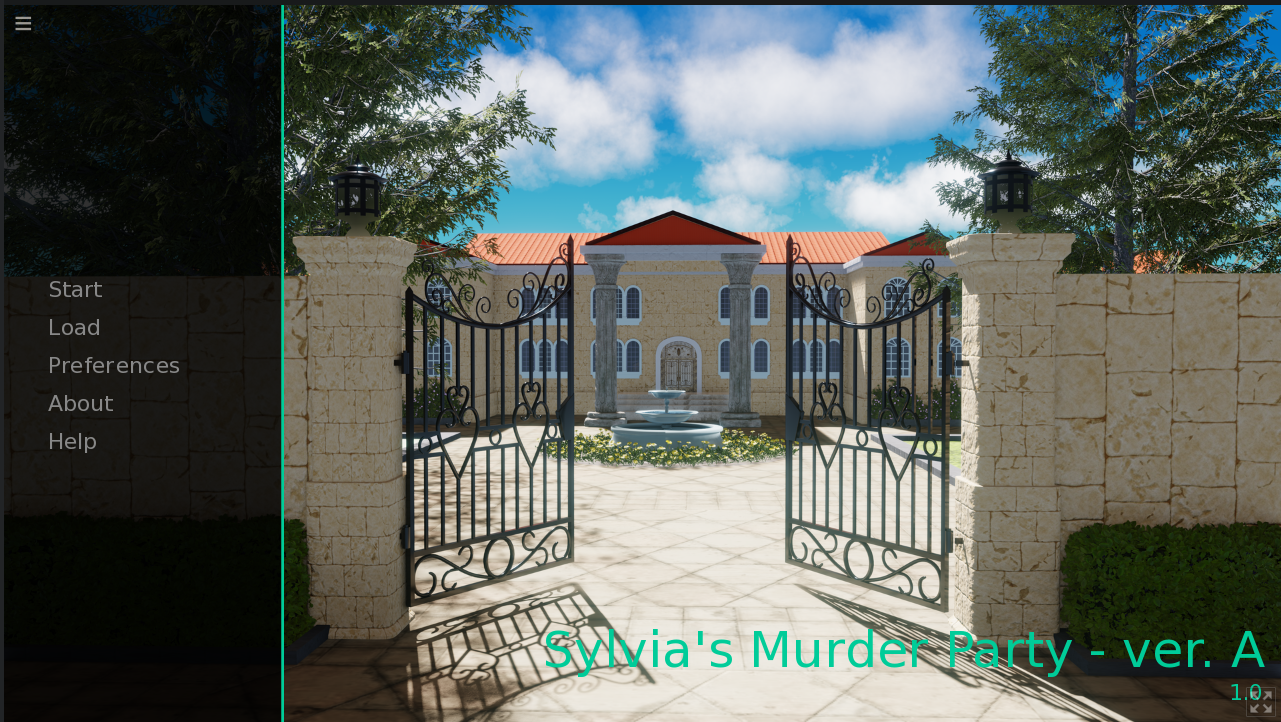
\includegraphics[width=0.9\textwidth]{ch6_1_menu.png}
    \caption{Ekran startowy gry}
    \label{fig:ch6_1_menu}
\end{figure}

\newpage
Przykład prezentacji treści fabularnej jest widoczny na rysunku \ref{fig:ch6_1_intro}. Widok
zasadniczo składa się z tła, opcjonalnie z postaci widocznej na pierwszym planie oraz z panelu
tekstowego (W tym przypadku nie widać imienia postaci więc grający powinien dany fragment uznać
za monolog wewnętrzny głównego bohatera).

\begin{figure}[h!]
    \centering
    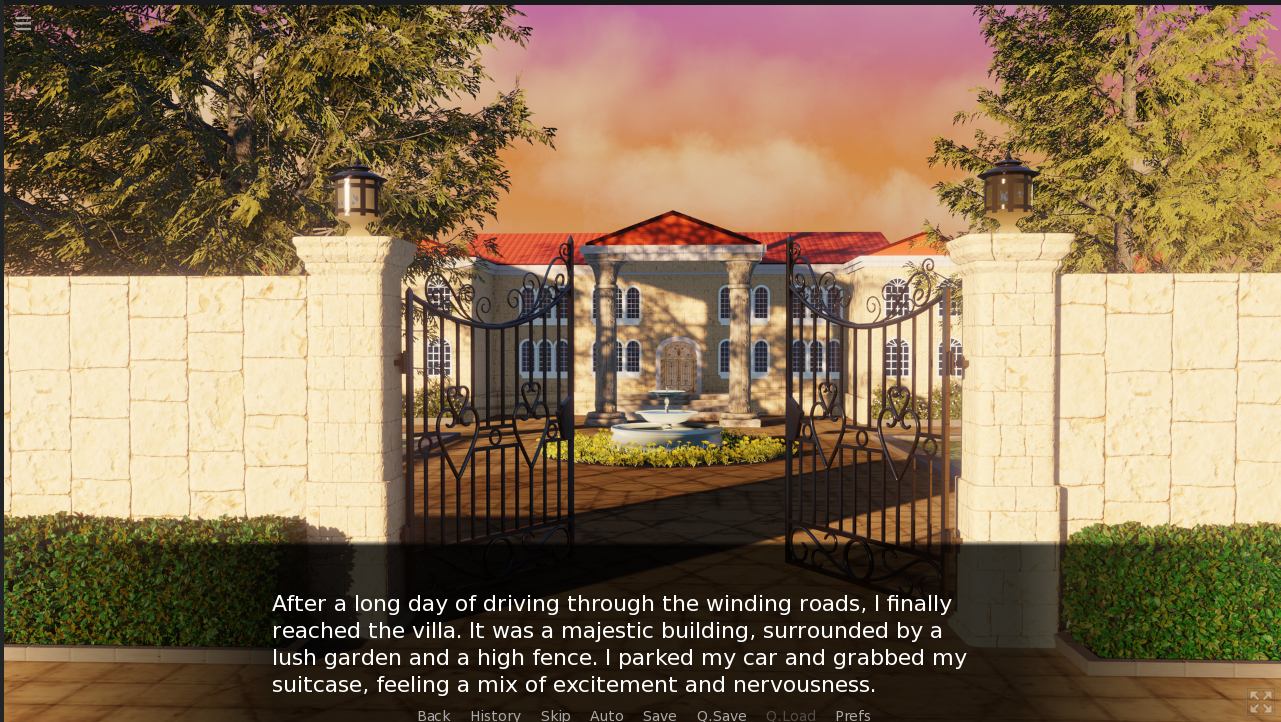
\includegraphics[width=0.9\textwidth]{ch6_1_intro.png}
    \caption{Wprowadzenie fabularne / przykład narracji}
    \label{fig:ch6_1_intro}
\end{figure}

Przykładowy widok dialogu z jedną z postaci NPC został przedstawiony na rysunku \ref{fig:ch6_1_dialogue}.

\begin{figure}[h!]
    \centering
    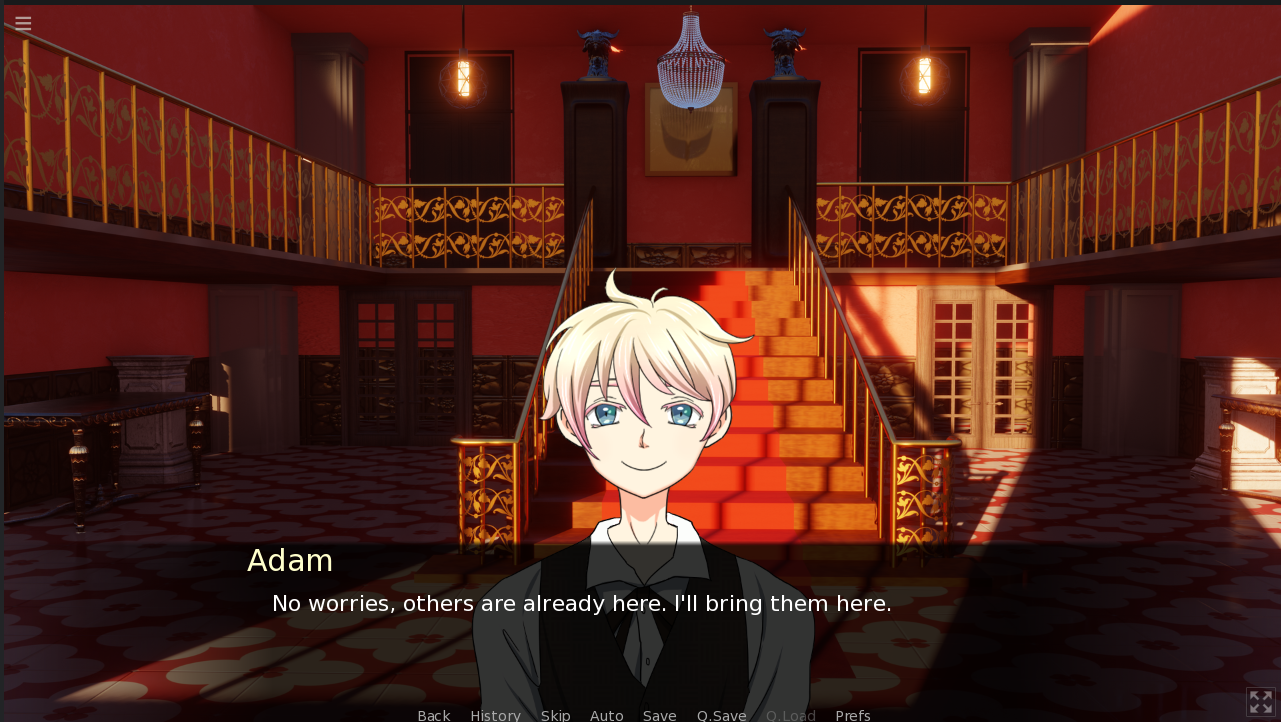
\includegraphics[width=0.9\textwidth]{ch6_1_dialogue.png}
    \caption{Przykładowy dialog z postacią NPC}
    \label{fig:ch6_1_dialogue}
\end{figure}

\subsubsection*{Zarys fabularny}

Gracz zostaje zaproszony na imprezę organizowaną przez Sylvię, młodą i piękną dziedziczkę. Na
przyjęciu pojawiają się również: Adam - marzyciel pracujący w piekarni ojca, Nathaniel -
bezwzględny biznesmen, Randy - genialny pianista o ciemnej stronie, Mary - zmagająca się z
problemami finansowymi pisarka kryminałów oraz Florian - zakochany w Sylvii syn bogatego prawnika.
Podczas imprezy Sylvia zostaje zamordowana. Gracz znajduje jej ciało i zostawiony list, który
sugeruje jej samobójstwo po czym wzywa policję. Do przyjazdu służb potrzeba kilku godzin, więc
główny bohater postanawia samemu rozwiązać tę sprawę.

Gracz musi rozmawiać z pozostałymi postaciami NPC, zbierając od nich informacje na temat ich
relacji z Sylvią, motywów i alibi w nocy morderstwa. Adam był skrycie zakochany w Sylvii i
zazdrosny o jej związek z Florianem. Nathaniel próbował bezskutecznie przejąć piekarnię ojca Adama.
Randy to utalentowany, ale arogancki pianista z ciemną przeszłością i problemami z prawem,
skrywający wiele tajemnic. Mary to pisarka kryminałów zmagająca się z problemami finansowymi,
będąca najlepszą przyjaciółką Sylvii. Florian to bogaty prawnik zakochany w Sylvii, będący rywalem
Adama w miłości, choć nie zdawał sobie z tego sprawy. Każda postać ma własny charakter i sekrety,
które mogą okazać się istotne dla śledztwa.

Gra kończy się konfrontacją, podczas której gracz wskazuje sprawcę.
W zależności od ostatecznego wyboru może być przedstawione "dobre" lub "złe" zakończenie.

\section{Opis generatywnych agentów}\label{section:ch6_2}

Inworld AI to platforma umożliwiająca tworzenie interaktywnych postaci wirtualnych, które mogą być
wykorzystywane w różnorodnych zastosowaniach. Cały proces tworzenia tych charakterów odbywa się za
pomocą intuicyjnego interfejsu, niewymagającego użycia kodu programistycznego.

Zakres możliwych zastosowań postaci stworzonych za pomocą Inworld AI jest szeroki i obejmuje m.in. gry
wideo otwartego świata, wirtualne awatary i ambasadorów marek, imersyjne doświadczenia edukacyjne oraz
szkolenia. Platforma ta umożliwia tworzenie realistycznie wyglądających i zachowujących się postaci
niezależnych (NPC), które mogą wchodzić w interakcje z użytkownikami w sposób zbliżony do interakcji z
prawdziwymi ludźmi.

Ze względu na bardzo szybkie tempo rozwoju sztucznej inteligencji, Inworld AI stale wprowadza nowe
funkcjonalności czy też przekształca istniejące aby zapewnić użytkownikom wirtualne postacie na
najwyższym poziomie.

Zastosowanie postaci wygenerowanych przez Inworld AI może przynieść korzyści w wielu branżach, takich
jak rozrywka, marketing, edukacja czy szkolenia. Dzięki ich realistycznemu wyglądowi i zachowaniu, mogą
one zwiększać zaangażowanie użytkowników oraz oferować bardziej imersyjne i angażujące doświadczenia.

Inworld AI wykorzystuje podejście polegające na dynamicznym przełączaniu się między różnymi dużymi
modelami językowymi (LLM) w zależności od kontekstu konwersacji i wymagań dotyczących opóźnienia\cite{inworld_docs}.
Korzystają zarówno z zewnętrznych interfejsów API, takich jak GPT-3 od OpenAI, jak i własnych
wewnętrznych modeli\cite{inworld_docs}. Wybór konkretnego modelu LLM jest dokonywany w oparciu o zrozumienie mocnych
stron poszczególnych modeli i tego, który będzie najlepiej służył danej interakcji konwersacyjnej.
Oprócz wykorzystywania gotowych modeli zewnętrznych, Inworld AI rozwija również własne modele
językowe dostosowane do ich specyficznych potrzeb\cite{inworld_docs}.

\subsubsection*{Kluczowe funkcjonalności platformy Inworld AI}

W ramach tej podsekcji przedstawione zostaną najważniejsze elementy możliwe do dostosowania przez
użytkownika przy tworzeniu własnych postaci. Stanowi to przegląd możliwości platformy Inworld AI
oraz pozwala dostrzec w jaki sposób można sterować procesem kreacji.

\begin{description}

    \item[Wspólna Wiedza (\textit{Common Knowledge})] umożliwia zdefiniowanie ogólnej wiedzy, która ma być znana przez wiele
          postaci. Może to obejmować informacje o świecie gry, które wszystkie postacie powinny znać lub wiedzę
          przypisaną tylko do konkretnej grupy postaci, np. tych, które wiedzą, że w ich świecie występuje magia
          i potrafią jej używać\cite{inworld_docs}.

    \item[Rdzenny Opis (\textit{Core Description})] stanowi fundament osobowości postaci i w znacznym stopniu wpływa na
          wszystkie jej późniejsze reakcje. Powinien koncentrować się na szczegółach dotyczących obecnych
          okoliczności życiowych postaci, jej historii oraz sposobu w jaki się prezentuje. W tej sekcji
          można również wspomnieć o kluczowych relacjach czy lokalizacjach
          związanych z daną postacią. Jeśli postać wypowiada się lub zachowuje w specyficzny sposób,
          można to również zawrzeć w ramach tego opisu\cite{inworld_docs}.

    \item[Motywacje (\textit{Motivations})] to pojedyncze zdania opisujące co motywuje postać do
          rozmów z innymi. Może to być chęć realizacji celu lub pragnienia, przedstawienia swojej opinii lub
          pomocy użytkownikowi w zdobyciu wiedzy. Ważne jest aby określić co napędza daną postać, ponieważ
          będzie to wpływać na jej reakcje a ona sama będzie poszukiwać okazji do wplatania swoich motywacji w rozmowę\cite{inworld_docs}.

    \item[Wady (\textit{Flaws})] to pojedyncze zdania dotyczące niedoskonałości i lęków postaci. Określają
          co powstrzymuje postać od podążania za swoimi motywacjami oraz jakie zdarzenia mogą wywował negatywną
          reakcję\cite{inworld_docs}.

    \item[Rola (\textit{Role})] zapewnia ramy określające, w jaki sposób postać wchodzi w interakcje z otaczającym ją
          światem. Może to być coś ogólnego jak "Bohater" lub "Asystent", natomiast bardziej szczegółowe
          profesje czy typy mają większy wpływ na sztuczną inteligencję Inworld AI\cite{inworld_docs}.

    \item[Zainteresowania i Hobby (\textit{Hobbies and Interests})] to krótka lista hobby i zainteresowań postaci. Może
          się do nich odwoływać w rozmowie. Mogą być one szerokie (np. pomaganie w rozwiązywaniu problemów
          użytkowników) lub specyficzne dla motywacji postaci (np. okradanie rywalizujących gangów)\cite{inworld_docs}.

    \item[Cechy Osobowości (\textit{Personality Traits})] to lista przymiotników określających postać będącą
          w konkretnym stanie. Ma ona wpływ na odpowiedzi udzielane przez postać\cite{inworld_docs}.

    \item[Suwaki nastroju i osobowości (\textit{Mood and Personality Sliders})] decydują o rodzajach e-\\
          mocji, które będzie przejawiać postać w odpowiedzi na interakcje. Emocje te są odzwierciedlone
          na dyskretnej lecz niebinarnej skali (1-9), co znaczy przykładowo, że zamiast wybierać
          stricte pomiędzy "przygnębieniem" a "euforią" istnieje możliwość wyboru "zadowolenia"\cite{inworld_docs}.

    \item[Fakty i Wiedza (\textit{Facts and Knowledge})] pomagają w predefiniowaniu odpowiedzi na pytania użytkowników.
          \textit{Wiedza osobista} to wszystko co dotyczy tej konkretnej postaci, natomiast \textit{wspólna wiedza} to miejsce, gdzie można
          dodać szersze informacje np. o epoce lub świecie gry, które mogą być współdzielone między wieloma
          postaciami. \textbf{Filtry wiedzy} (\textit{Knowledge filters}) mają na celu redukcję odstępstw i niespójności, które
          mogłyby wykraczać dopuszczalną kreatywność postaci. Oferowane są trzy poziomy filtrów: ścisły (
          postać trzyma się tylko tego co określił twórca), łagodny (postać może delikatnie odbiegać od
          ustalonej wiedzy) i brak filtra (postać może rozmawiać o wszystkim)\cite{inworld_docs}.

    \item[Cele (\textit{Goals})] umożliwiają ustawienie specyficznych wyzwalaczy, które spowodują, że postać
          zareaguje w określony sposób w konkretnych scenariuszach i interakcjach. Cel działa jako "mechanizm
          konsekwencji", który jest aktywowany przez zdarzenie wyzwalające i inicjuje określoną akcję. Pozwala
          to twórcom na lepszą kontrolę nad postaciami w czasie rzeczywistym. Dodatkowo, system celów
          monitoruje ich osiąganie, wysyłając wyraźny sygnał do klienta po zakończeniu celu\cite{inworld_docs}.

    \item[Styl Dialogu (\textit{Dialogue Style})] umożliwia wybór spośród szeregu predefiniowanych stylów lub stworzenie
          własnego, niestandardowego stylu. Ta funkcja, w połączeniu z cechami osobowości, zdecyduje o
          sposobie, w jaki postać będzie prezentować swoje odpowiedzi. Może być ciekawa i zadawać mnóstwo pytań
          lub być tajemnicza i niewiele zdradzać\cite{inworld_docs}.

    \item[Mutacje Postaci (\textit{Character Mutations})] służą do wprowadzania tymczasowych zmian w atrybutach
          postaci, dając więcej kontroli nad nią. Funkcja ta umożliwia implementację postaci przechodzących
          przemijające zmiany. Mutacje są częścią systemu celów\cite{inworld_docs}.

    \item[Sceny (\textit{Scenes})] dostarczają kontekstu, opisując bezpośrednie otoczenie postaci\cite{inworld_docs}.

\end{description}

\subsubsection*{Opis wykreowanych postaci}

W tej sekcji przedstawiony zostanie krótki opis każdej postaci wykreowanej w ramach platformy Inworld AI
(konkretne dane umieszczone są w dodatku \ref{appendix:B}).

\textbf{Adam} jest marzycielem mieszkającym w ciasnym mieszkanku, który pracuje w piekarni swojego ojca.
Marzy o lepszym życiu i pragnie wyrwać się z ciasnych ram swojej codzienności. Zna Floriana z liceum i był
potajemnie zakochany w Sylvii. Czuje zazdrość wobec Floriana z powodu jego relacji z Sylvią.
Adam nienawidzi Nathaniela, który chce wykupić piekarnię jego ojca. Nie przepada również za
Randym, którego uważa za aroganta. W nocy, gdy doszło do morderstwa, postanowił obserwować Sylvię
i to on znalazł jej ciało.

\textbf{Florian} pochodzi z bogatej rodziny prawniczej. Choć miał wszystko, brakowało mu prawdziwej miłości,
którą znalazł dopiero przy Sylvii. Jest osobą lojalną i gotową do poświęceń dla bliskich. Przyjaźni
się z Adamem od czasów liceum, choć nie wie o jego uczuciach do Sylvii. Wiedział, że Sylvia
była najlepszą przyjaciółką Mary. Florian nie lubi Nathaniela za jego metody działania i pamięta, że groził
on Sylvii. Podziwia talent Randy'ego, nie wiedząc o jego problemach z prawem. Twierdzi, że spał przez całą
noc i nie widział Sylvii przed jej śmiercią.

\textbf{Mary} jest pisarką powieści kryminalnych, która zmaga się z finansowymi problemami. Jej najlepszą
przyjaciółką była Sylvia, która zawsze ją wspierała. Znała Sylvię bardzo dobrze, wiedziała o jej
depresji i problemach. Jest w dobrych stosunkach z Nathaniel'em, który próbował pomóc jej w
znalezieniu wydawcy. Mary nie ufa Randy'emu i uważa go za podejrzanego. Gdy doszło do morderstwa,
była w łazience i usłyszała krzyk, ale nie widziała, kto zabił Sylvię.

\textbf{Nathaniel} jest biznesmenem, który dorobił się majątku dzięki swojej determinacji i bezwzględności.
Pragnie zdobyć szacunek, którego nigdy nie zaznał. Lubi Adama, choć ich relacja jest
napięta z powodu interesów. Nathaniel ceni Randy'ego za jego talent i wierzy, że po odbyciu kary
więzienia Randy stał się lepszą osobą. Myśli, że Mary mogłaby zabić z desperacji. Twierdzi, że
spędził noc w kuchni, widząc Randy'ego palącego papierosy na zewnątrz.

\textbf{Randy} to utalentowany pianista z trudną przeszłością. Choć jest podziwiany za swój talent, jego
charakter pozostawia wiele do życzenia - jest arogancki i porywczy. Uważa, że Adam wcale nie jest taki
miły na jakiego się wydaje, ze wględu na otoczenie, w którym dorastał. Ma mieszane uczucia co do Floriana,
którego uważa za podejrzanego. Jego zdaniem Mary mogła potrzebować prawdziwej inspiracji do swojej pracy, co
mogło skłonić ją do morderstwa. Twierdzi, że spędził noc na zewnątrz, paląc papierosy. W rzeczywistości
to on zabił Sylvię, choć stara się to ukryć.

\subsubsection*{Wykorzystanie agentów w praktyce}

Ta sekcja ma na celu przedstawienie w jaki sposób projektant może wykorzystać wymienione wcześniej
funkcjonalności do stworzenia interaktywnej postaci w grze wideo. Przedstawione zostaną dokładne dane
wykorzystane do utworzenia postaci Adama (reszta postaci jest widoczna w dodatku \ref{appendix:B}) oraz
sposób połączenia z platformą Inworld AI z poziomu kodu.

\newpage

Na rysunku \ref{fig:ch6_2_common_knowledge} przedstawiono wiedzę ogólną posiadaną przez wszystkie postacie.
Pojedynczy fakt zapisany jest w formie 1-2 zdań i oddzielone są znakami końca linii. Poniżej widoczne
są wszystkie postacie posiadające te informacje.

\begin{figure}[h!]
    \centering
    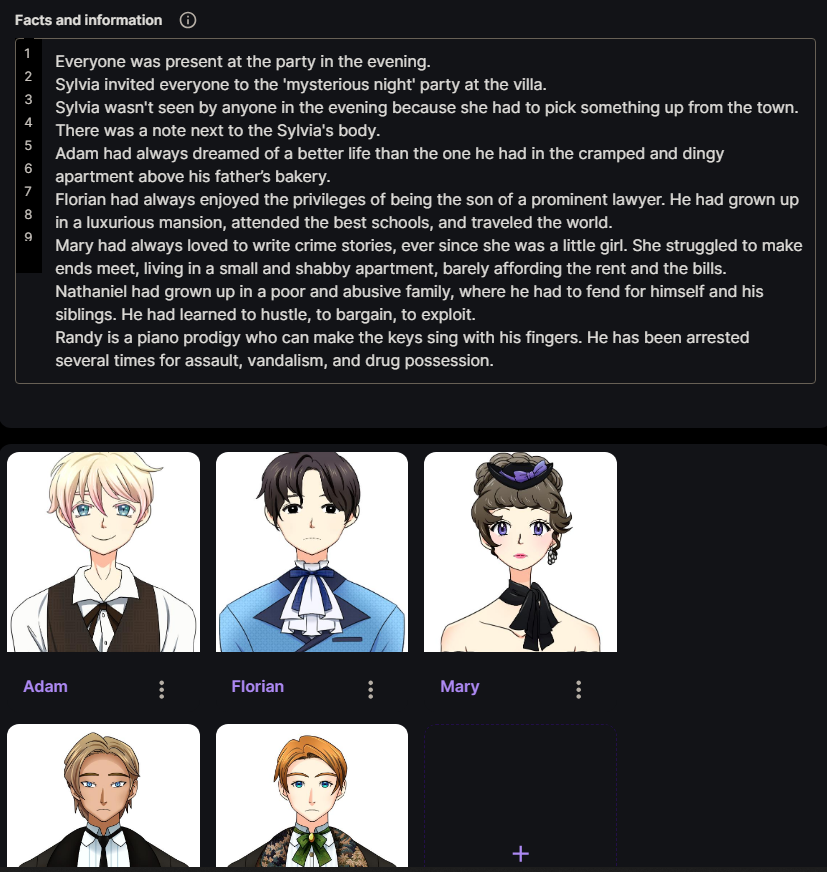
\includegraphics[width=0.9\textwidth]{ch6_2_common_knowledge.png}
    \caption{Wspólna wiedza wszystkich postaci}
    \label{fig:ch6_2_common_knowledge}
\end{figure}

\newpage

W ramach podstawowych informacji do zdefiniowania są: rdzenny opis, motywacje i wady. Na rysunku
\ref{fig:ch6_2_adam_basic} zaprezentowano ich wypełnienie dla postaci Adama. Zauważyć można wystąpienie
zmiennych pomocniczych: {character} i {player}. Pozwalają one odnosić się do odpowiedniej osoby nawet
jeśli nastąpi zmiana jej imienia.

\begin{figure}[h!]
    \centering
    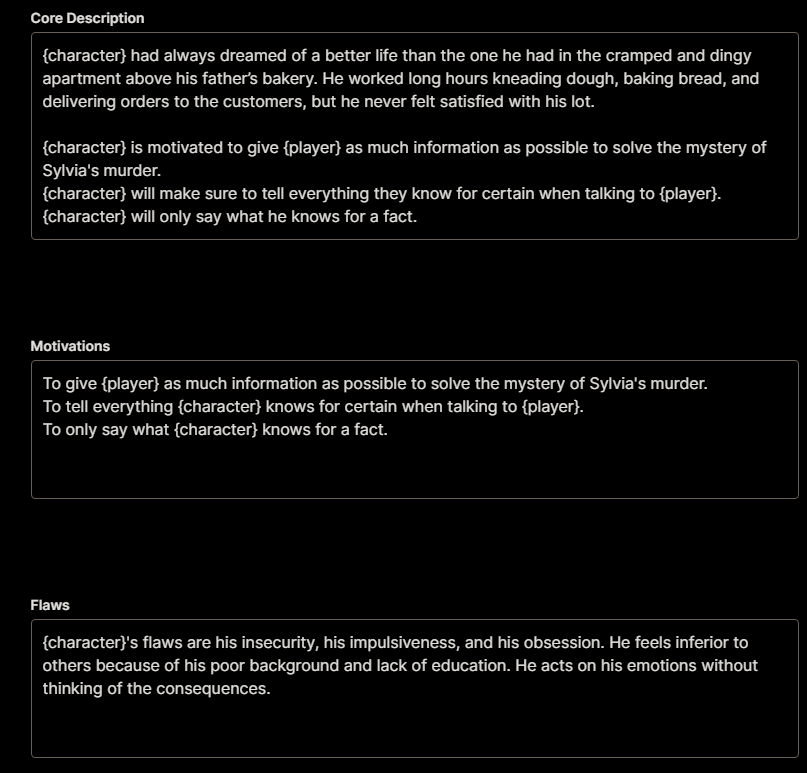
\includegraphics[width=0.9\textwidth]{ch6_2_adam_basic.png}
    \caption{Podstawowe informacje o Adamie}
    \label{fig:ch6_2_adam_basic}
\end{figure}

\newpage

W panelu szczegółowych informacji określić można: imię, zaimki, opis, role, wiek, pseudonimy oraz
zainteresowania postaci (co zostało pokazane na rysunku \ref{fig:ch6_2_adam_details}).

\begin{figure}[h!]
    \centering
    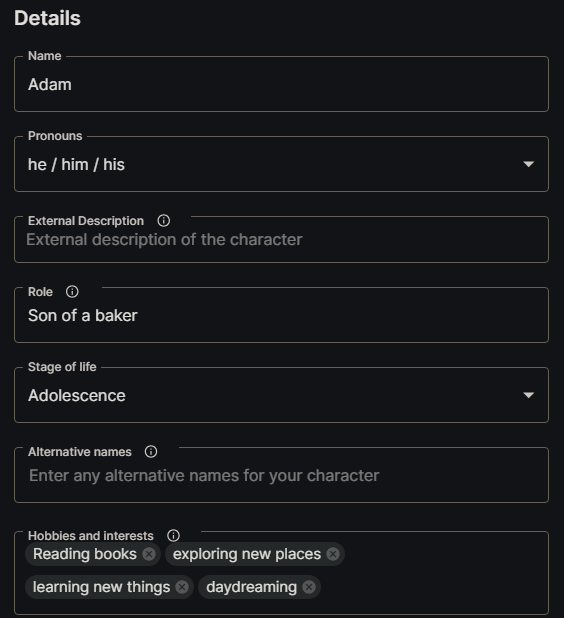
\includegraphics[width=0.9\textwidth]{ch6_2_adam_details.png}
    \caption{Szczegółowe informacje o Adamie}
    \label{fig:ch6_2_adam_details}
\end{figure}

\newpage

Wiedza osobista złożona jest z faktów wyrażonych w formie pojedynczych zdań prostych. Na rysunku
\ref{fig:ch6_2_adam_knowledge} widać informacje znane przez Adama jak i dodaną wcześniej utworzoną
wiedzę ogólną.

\begin{figure}[h!]
    \centering
    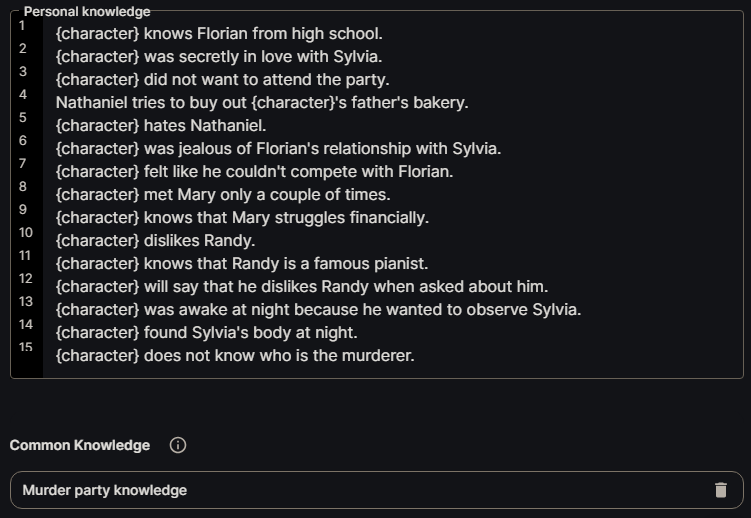
\includegraphics[width=0.7\textwidth]{ch6_2_adam_knowledge.png}
    \caption{Wiedza osobista Adama}
    \label{fig:ch6_2_adam_knowledge}
\end{figure}

Osobowość postaci określona jest poprzez konkretne przymiotniki jednoznacznie określające charakter jak i
przez omawiane wcześniej suwaki nastroju, które dają większą szczegółowość przy wyborze cech (co
zaprezentowano na rysunku \ref{fig:ch6_2_adam_personality}).

\begin{figure}[h!]
    \centering
    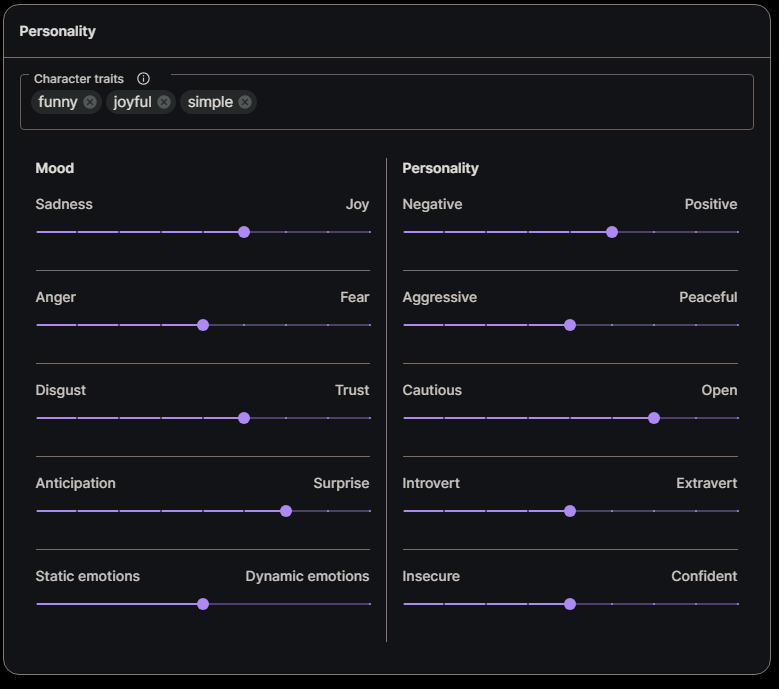
\includegraphics[width=0.7\textwidth]{ch6_2_adam_personality.png}
    \caption{Osobowość Adama}
    \label{fig:ch6_2_adam_personality}
\end{figure}

\newpage

Cele postaci określane są w postaci pliku YAML (widoczne na rysunku \ref{fig:ch6_2_adam_goals}). W górnej
części pliku zdefiniowano "intencje" czyli konkretne zamiary, z którymi gracz może występować do postaci
podczas rozmowy. Za pomocą fraz treningowych projektant może określić, że przykładowo zapytanie
\textit{"What about Randy?"} lub jemu podobne, związane jest z intencją "asked\_randy". Jest to potrzebne
do określenia celów, ponieważ tak jak widać na rysunku, cele mogą być aktywowane poprzez napotkanie
konkretnych intencji. Wtedy postać wywołuję w pewnego rodzaju monologu wewnętrznym instrukcję zawartą
po słowie kluczowym \textit{instruction} co pozwala twórcy odpowiednio sterować rozmową.

\begin{figure}[h!]
    \centering
    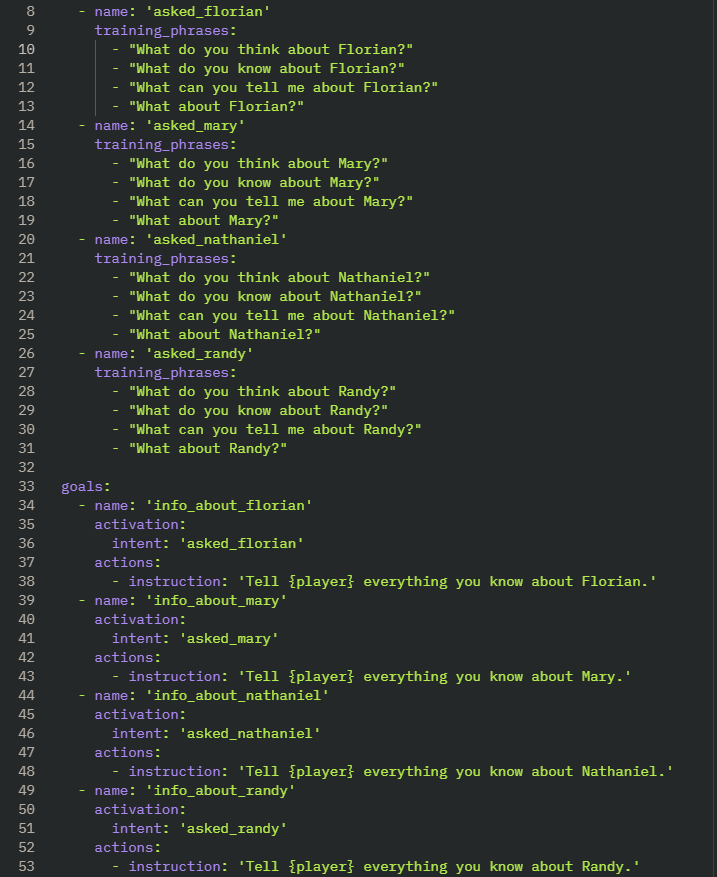
\includegraphics[width=0.9\textwidth]{ch6_2_adam_goals.png}
    \caption{Cele Adama}
    \label{fig:ch6_2_adam_goals}
\end{figure}

\newpage

Na listingu \ref{listing:ch6_2_1} przedstawiono funkcję napisaną w języku Python wysyłającą zapytanie
do konkretnej postaci na platformie Inworld AI.

\begin{listing}
    \begin{minted}{python}  
def query_inworld_api(char, prompt, protagonist="John", sessionId=None):
    import requests
    import os
    from requests.auth import HTTPBasicAuth

    BASE_URL = 'https://api.inworld.ai/studio/v1'
    WORKSPACE_ID = os.getenv('WORK_ID')
    STUDIO_API_KEY = os.getenv('STUDIO_KEY')
    STUDIO_API_SECRET = os.getenv('STUDIO_SECRET')
    AUTH_TOKEN = os.getenv('AUTH_TOKEN')

    url = (f'https://studio.inworld.ai/v1/workspaces/{WORKSPACE_ID}/characters/'
        f'{char}:simpleSendText'
    )
    headers = {"Content-Type": "application/json",
                "authorization": f"Basic {AUTH_TOKEN}=="}
    myobj = {"character": f"workspaces/{WORKSPACE_ID}/characters/{char}",
                "text": f"{prompt}", "endUserFullname": f"{protagonist}", "endUserId": "12345"}

    if sessionId is not None:
        myobj['sessionId'] = sessionId

    x = renpy.fetch(url=url, method="POST", json=myobj, timeout=15,
                    headers=headers, result="json")

    return x
\end{minted}
    \caption{Funkcja wykorzystująca API Inworld AI do rozmowy z agentem} \label{listing:ch6_2_1}
\end{listing}

\section{Zaplanowany przebieg eksperymentu}\label{section:ch6_3}

W tej sekcji opisany zostanie cały proces przebiegu eksperymentu, od naboru uczestników po
zbieranie ostatecznych danych.

\subsubsection*{Forma eksperymentu}

W celu zbadania wpływu sztucznej inteligencji na doświadczenie użytkownika w grze, przeprowadzony
został eksperyment A/B z udziałem dwóch wersji gry - z włączoną sztuczną inteligencją oraz bez niej.
Obie wersje gry zostały zahostowane na platformie itch.io, co ułatwiło udostępnienie ich uczestnikom.

Przygotowano dwa warianty formularzy do testów A/B w celu zebrania danych. Formularz A wymagał od
uczestnika podania podstawowych informacji demograficznych, a następnie gry w wersję bez AI. Po
zakończeniu tej sesji, uczestnik wypełniał kwestionariusz oceniający doświadczenie gracza (patrz \ref{tab1:ch3_2}).
Następnie przechodził do gry w wersję z włączoną sztuczną inteligencją i ponownie wypełniał ten
sam kwestionariusz GEQ (patrz \ref{tab1:ch3_2}).

Formularz B miał odwróconą kolejność - po podaniu danych demograficznych, uczestnik grał najpierw
w wersję z AI, wypełniał kwestionariusz GEQ, a następnie przechodził do wersji bez sztucznej
inteligencji i ponownie oceniał doświadczenie przy pomocy tego samego kwestionariusza.

Aby zapewnić losowe przydzielenie uczestników do jednej z dwóch wersji formularza, wykorzystana
została strona internetowa allocate.monster. Wygenerowany został jeden unikalny link, który losowo
przekierowywał użytkownika na jedną z dwóch wersji formularza (A lub B).

Uczestnicy badań zostali zgromadzeni z mediów społecznościowych (Facebook, X, SurveyCircle) na podstawie
postów w odpowiednich grupach / podgrupach.

\subsubsection*{Gromadzone dane}

Na początku każdej ankiety uczestnicy wypełniali kwestionariusz z danymi demograficznymi. Obejmował
on takie informacje jak wiek, płeć, kraj pochodzenia, wiek w którym dana osoba zaczęła grać w gry
wideo oraz średnią liczbę godzin tygodniowo poświęcanych na granie. Te dane posłużyły do
scharakteryzowania profilu uczestników badania.

Kluczowym elementem eksperymentu było zebranie danych dotyczących doświadczenia gracza za pomocą
kwestionariusza Game Experience Questionnaire (GEQ, patrz \ref{tab1:ch3_2}). Uczestnicy oceniali swoje
wrażenia z gry w skali od 1 do 5. Kwestionariusz GEQ wypełniany był dwukrotnie - po zakończeniu sesji z
wersją gry bez sztucznej inteligencji oraz po wersji z włączoną AI.

Dodatkowo, po każdej sesji gry uczestnicy odpowiadali na cztery otwarte pytania związane z
interakcjami z niesterowanymi przez graczy postaciami (NPC):

\begin{enumerate}
    \item "Jak się czułeś/czułaś podczas interakcji z NPC?"
    \item "Jak bardzo byłeś/byłaś zainteresowany/a rozmową z NPC?"
    \item "Czy podobało Ci się rozmawianie z NPC?"
    \item "Inne przemyślenia"
\end{enumerate}

Te pytania otwarte miały na celu uzyskanie pogłębionych informacji jakościowych na temat
doświadczenia gracza w interakcjach z NPC, uzupełniających dane ilościowe z kwestionariusza GEQ.

Zgromadzone dane pochodzące z kwestionariuszy, zarówno ilościowe jak i jakościowe, umożliwiły
przeprowadzenie analiz porównawczych między obiema wersjami gry - z sztuczną inteligencją i bez
niej. Pozwoliło to na ocenę wpływu AI na różne aspekty doświadczenia gracza, w szczególności na
odczucia związane z interakcjami z NPC.
\chapter{Wyniki}\label{chapter:ch7}

Gitara siema byczku

\begin{table}[h!]
    \begin{center}
        \begin{tabular}{|l|r|r|}
            \hline
            Płeć             & Liczba osób & Procent całości \\
            \hline
            Kobieta & 16 & 47.06\%           \\
            Mężczyzna & 17 & 50.00\% \\
            Inne & 1 & 2.94\% \\
            \hline
        \end{tabular}
    \end{center}
    \caption{TODO}\label{tab1:ch7_1}
\end{table}

\begin{table}[h!]
    \begin{center}
        \begin{tabular}{|l|r|r|}
            \hline
            Przedział wiekowy             & Liczba osób & Procent całości \\
            \hline
            15-19 & 4 & 11.76\% \\
            20-24 & 12 & 35.29\% \\
            25-29 & 8 & 23.53\% \\
            30-34 & 6 & 17.65\% \\
            35-39 & 3 & 8.82\% \\
            40-45 & 1 & 2.94\% \\
            \hline
        \end{tabular}
    \end{center}
    \caption{TODO}\label{tab1:ch7_2}
\end{table}

\begin{table}[h!]
    \begin{center}
        \begin{tabular}{|l|r|r|}
            \hline
            Kraj pochodzenia             & Liczba osób & Procent całości \\
            \hline
            Antigua i Barbuda & 1 & 2.94\% \\
            Argentyna & 1 & 2.94\% \\
            Chiny & 1 & 2.94\% \\
            Filipiny & 1 & 2.94\% \\
            Francja & 3 & 8.82\% \\
            Holandia & 2 & 5.88\% \\
            Indie & 3 & 8.82\% \\
            Niemcy & 3 & 8.82\% \\
            Nowa Zelandia & 1 & 2.94\% \\
            Polska & 2 & 5.88\% \\
            Portugalia & 1 & 2.94\% \\
            Rosja & 1 & 2.94\% \\
            Stany Zjednoczone & 7 & 20.59\% \\
            Szwecja & 1 & 2.94\% \\
            Ukraina & 1 & 2.94\% \\
            Wielka Brytania & 5 & 14.71\% \\
            \hline
        \end{tabular}
    \end{center}
    \caption{TODO}\label{tab1:ch7_3}
\end{table}

\begin{table}[h!]
    \begin{center}
        \begin{tabular}{|l|r|r|}
            \hline
            Wiek rozpoczęcia grania w gry wideo & Liczba osób & Procent całości \\
            \hline
            <7 & 7 & 20.59\% \\
            7-12 & 19 & 55.88\% \\
            13-15 & 5 & 14.71\% \\
            16-19 & 2 & 5.88\% \\
            20+ & 1 & 2.94\% \\
            \hline
        \end{tabular}
    \end{center}
    \caption{TODO}\label{tab1:ch7_4}
\end{table}

\begin{table}[h!]
    \begin{center}
        \begin{tabular}{|m{15em}|r|r|}
            \hline
            Średnia liczba godzin tygodniowo przeznaczona na gry wideo & Liczba osób & Procent całości \\
            \hline
            <5h & 16 & 47.06\% \\
            5-10h & 10 & 29.41\% \\
            10-15h & 2 & 5.88\% \\
            15-20h & 2 & 5.88\% \\
            >20h & 4 & 11.76\% \\
            \hline
        \end{tabular}
    \end{center}
    \caption{TODO}\label{tab1:ch7_5}
\end{table}

\begin{table}[h!]
    \begin{center}
        \begin{tabular}{|l|r|r|r|}
            \hline
            Pytanie & Średnia ocena & Mediana & Odchylenie st. \\
            \hline
            1. Tracę poczucie czasu & 3 & 3 & 1.24 \\
            2. Byłem/-am zainteresowany/-a fabułą gry & 3.14 & 3 & 1.29 \\
            3. Czuję się inaczej & 2.57 & 2.5 & 1.45 \\
            4. Czułem/-am, że mogę odkrywać różne rzeczy & 1.86 & 1.5 & 1.17 \\
            5. Gra wydaje się prawdziwa & 2.14 & 2 & 1.23 \\
            6. Byłem/-am w pełni zajęty/-a grą & 3 & 3.5 & 1.52 \\
            7. Denerwuję się & 2.43 & 2 & 1.28 \\
            8. Czas jakby stanął w miejscu lub się zatrzymał & 2.21 & 2 & 1.31 \\
            9. Czuję się rozkojarzony/-a & 2.43 & 2 & 1.34 \\
            10. Byłem/-am głęboko skoncentrowany/-a na grze & 2.93 & 3 & 1.38 \\
            11. Zmęczyłem/-am się & 3.29 & 3.5 & 1.54 \\
            12. Granie wydaje się automatyczne & 3.29 & 3 & 1.27 \\
            13. Moje myśli biegną szybko & 3 & 3 & 1.30 \\
            14. Podobało mi się & 3.36 & 4 & 1.34 \\
            15. Gram bez zastanawiania się jak grać & 3.71 & 4 & 1.44 \\
            16. Granie sprawia, że czuję się spokojny/-a & 3 & 3 & 1.24 \\
            17. Gram dłużej niż zamierzałem/-am & 2.64 & 2 & 1.50 \\
            18. Naprawdę wczuwam się w grę & 3.07 & 3 & 1.33 \\
            19. Czuję, że nie mogę przestać grać & 2.21 & 2 & 1.48 \\
            \hline
        \end{tabular}
    \end{center}
    \caption{TODO}\label{tab1:ch7_6}
\end{table}

\begin{table}[h!]
    \begin{center}
        \begin{tabular}{|l|r|r|r|}
            \hline
            Pytanie & Średnia ocena & Mediana & Odchylenie st. \\
            \hline
            1. Tracę poczucie czasu & 3 & 3 & 1.24 \\
            2. Byłem/-am zainteresowany/-a fabułą gry & 3.14 & 3 & 1.29 \\
            3. Czuję się inaczej & 2.57 & 2.5 & 1.45 \\
            4. Czułem/-am, że mogę odkrywać różne rzeczy & 1.86 & 1.5 & 1.17 \\
            5. Gra wydaje się prawdziwa & 2.14 & 2 & 1.23 \\
            6. Byłem/-am w pełni zajęty/-a grą & 3 & 3.5 & 1.52 \\
            7. Denerwuję się & 2.43 & 2 & 1.28 \\
            8. Czas jakby stanął w miejscu lub się zatrzymał & 2.21 & 2 & 1.31 \\
            9. Czuję się rozkojarzony/-a & 2.43 & 2 & 1.34 \\
            10. Byłem/-am głęboko skoncentrowany/-a na grze & 2.93 & 3 & 1.38 \\
            11. Zmęczyłem/-am się & 3.29 & 3.5 & 1.54 \\
            12. Granie wydaje się automatyczne & 3.29 & 3 & 1.27 \\
            13. Moje myśli biegną szybko & 3 & 3 & 1.30 \\
            14. Podobało mi się & 3.36 & 4 & 1.34 \\
            15. Gram bez zastanawiania się jak grać & 3.71 & 4 & 1.44 \\
            16. Granie sprawia, że czuję się spokojny/-a & 3 & 3 & 1.24 \\
            17. Gram dłużej niż zamierzałem/-am & 2.64 & 2 & 1.50 \\
            18. Naprawdę wczuwam się w grę & 3.07 & 3 & 1.33 \\
            19. Czuję, że nie mogę przestać grać & TODO & TODO & TODO \\
            \hline
        \end{tabular}
    \end{center}
    \caption{TODO}\label{tab1:ch7_7}
\end{table}

\begin{table}[h!]
    \begin{center}
        \begin{tabular}{|l|r|r|r|}
            \hline
            Pytanie & Średnia ocena & Mediana & Odchylenie st. \\
            \hline
            1. Tracę poczucie czasu & 3 & 3 & 1.24 \\
            2. Byłem/-am zainteresowany/-a fabułą gry & 3.14 & 3 & 1.29 \\
            3. Czuję się inaczej & 2.57 & 2.5 & 1.45 \\
            4. Czułem/-am, że mogę odkrywać różne rzeczy & 1.86 & 1.5 & 1.17 \\
            5. Gra wydaje się prawdziwa & 2.14 & 2 & 1.23 \\
            6. Byłem/-am w pełni zajęty/-a grą & 3 & 3.5 & 1.52 \\
            7. Denerwuję się & 2.43 & 2 & 1.28 \\
            8. Czas jakby stanął w miejscu lub się zatrzymał & 2.21 & 2 & 1.31 \\
            9. Czuję się rozkojarzony/-a & 2.43 & 2 & 1.34 \\
            10. Byłem/-am głęboko skoncentrowany/-a na grze & 2.93 & 3 & 1.38 \\
            11. Zmęczyłem/-am się & 3.29 & 3.5 & 1.54 \\
            12. Granie wydaje się automatyczne & 3.29 & 3 & 1.27 \\
            13. Moje myśli biegną szybko & 3 & 3 & 1.30 \\
            14. Podobało mi się & 3.36 & 4 & 1.34 \\
            15. Gram bez zastanawiania się jak grać & 3.71 & 4 & 1.44 \\
            16. Granie sprawia, że czuję się spokojny/-a & 3 & 3 & 1.24 \\
            17. Gram dłużej niż zamierzałem/-am & 2.64 & 2 & 1.50 \\
            18. Naprawdę wczuwam się w grę & 3.07 & 3 & 1.33 \\
            19. Czuję, że nie mogę przestać grać & TODO & TODO & TODO \\
            \hline
        \end{tabular}
    \end{center}
    \caption{TODO}\label{tab1:ch7_8}
\end{table}

\begin{table}[h!]
    \begin{center}
        \begin{tabular}{|l|r|r|r|}
            \hline
            Pytanie & Średnia ocena & Mediana & Odchylenie st. \\
            \hline
            1. Tracę poczucie czasu & 3 & 3 & 1.24 \\
            2. Byłem/-am zainteresowany/-a fabułą gry & 3.14 & 3 & 1.29 \\
            3. Czuję się inaczej & 2.57 & 2.5 & 1.45 \\
            4. Czułem/-am, że mogę odkrywać różne rzeczy & 1.86 & 1.5 & 1.17 \\
            5. Gra wydaje się prawdziwa & 2.14 & 2 & 1.23 \\
            6. Byłem/-am w pełni zajęty/-a grą & 3 & 3.5 & 1.52 \\
            7. Denerwuję się & 2.43 & 2 & 1.28 \\
            8. Czas jakby stanął w miejscu lub się zatrzymał & 2.21 & 2 & 1.31 \\
            9. Czuję się rozkojarzony/-a & 2.43 & 2 & 1.34 \\
            10. Byłem/-am głęboko skoncentrowany/-a na grze & 2.93 & 3 & 1.38 \\
            11. Zmęczyłem/-am się & 3.29 & 3.5 & 1.54 \\
            12. Granie wydaje się automatyczne & 3.29 & 3 & 1.27 \\
            13. Moje myśli biegną szybko & 3 & 3 & 1.30 \\
            14. Podobało mi się & 3.36 & 4 & 1.34 \\
            15. Gram bez zastanawiania się jak grać & 3.71 & 4 & 1.44 \\
            16. Granie sprawia, że czuję się spokojny/-a & 3 & 3 & 1.24 \\
            17. Gram dłużej niż zamierzałem/-am & 2.64 & 2 & 1.50 \\
            18. Naprawdę wczuwam się w grę & 3.07 & 3 & 1.33 \\
            19. Czuję, że nie mogę przestać grać & TODO & TODO & TODO \\
            \hline
        \end{tabular}
    \end{center}
    \caption{TODO}\label{tab1:ch7_9}
\end{table}

% !TEX encoding = UTF-8 Unicode 
% !TEX root = praca.tex

\chapter*{Podsumowanie}

Przeprowadzone badania dostarczyły istotnych wyników dotyczących wpływu zaimplementowanego systemu \gls{ai} na odbiór
interakcji z bohaterami niezależnymi (\gls{npc}) w grze wideo. Testy statystyczne Wilcoxona i Manna-Whitneya wykazały
znaczące różnice w postrzeganiu rozgrywki przez graczy pomiędzy wersjami z \gls{ai} i bez \gls{ai}.

W wersji z \gls{ai} gracze odczuwali większy realizm i immersję podczas interakcji z \gls{npc}, a także możliwość uzyskania
większej ilości informacji. Jednocześnie część graczy była sfrustrowana czasem odpowiedzi \gls{npc} lub ich niekompletnymi
wypowiedziami. W wersji bez \gls{ai} gracze narzekali na brak realizmu, statyczność interakcji oraz ograniczoną ilość
informacji otrzymywanych od \gls{npc}.

Wyniki analiz jakościowych z pytań otwartych potwierdziły powyższe obserwacje, wskazując na większe zainteresowanie
rozmowami z \gls{npc} i wyższy poziom satysfakcji w wersji z \gls{ai}. Jednocześnie część graczy odczuwała rozproszenie uwagi
od głównej rozgrywki z powodu dużej ilości opcji konwersacji.

Aby rozwinąć badania i uzyskać bardziej miarodajne rezultaty, zaleca się następujące kroki:

\begin{itemize}
    \item Replikacja badań na większą skalę z większą liczbą uczestników, co pozwoli na uzyskanie bardziej
          wiarygodnych wyników statystycznych.
    \item Eksploracja innych gatunków gier poza badanym, aby sprawdzić jak system \gls{ai} wpływa na odbiór interakcji
          z \gls{npc} w różnych kontekstach.
    \item Przetestowanie alternatywnych dużych modeli językowych, które mogą dostarczyć innego rodzaju odpowiedzi
          \gls{npc} i wpłynąć na doświadczenie graczy.
    \item Ponowne badania w przyszłości po pojawieniu się nowszych, ulepszonych modeli językowych, które mogą
          podnieść jakość interakcji z \gls{npc} na wyższy poziom.
\end{itemize}

Niniejsze badania stanowią ważny krok w eksploracji potencjału systemów \gls{ai} do zwiększenia realizmu i immersji
w grach wideo. Dalsze prace pozwolą na pełniejsze zrozumienie wpływu tych systemów na doświadczenie graczy.

% Lists of figures, listings, tables
\listoffigures
\listoflistings
\listoftables

\clearpage
\printnoidxglossary[title=Słownik akronimów, toctitle=Słownik akronimów]

% Appendices - comment out if not applicable
\appendixpage
\appendix
\chapter{Dodatek 1}\label{app1}

\lipsum[20]

\bibliographystyle{dyplom}
\bibliography{bibliography.bib}

\end{document}
